\documentclass[12pt,a4paper,ngerman]{article}
\usepackage{amsmath}
\usepackage{amsthm}
\usepackage{framed}
\usepackage{graphicx} 
\usepackage[utf8]{inputenc}
%Layout
\setlength{\topmargin}{1pt} \setlength{\headheight}{0.3cm}
\setlength{\textwidth}{16.5cm} \setlength{\textheight}{23cm}
\setlength{\oddsidemargin}{0cm} \setlength{\evensidemargin}{0cm}
\setlength{\headsep}{2pt} \setlength{\parindent}{0pt}
\setlength{\marginparwidth}{80pt} \pagestyle{plain}

\title{Physik TE \\
Ausarbeitung und Zusammenfassung}
\author{Martin Winter}
\date{08.09.2014 - 14.09.2014}

\begin{document}
  \maketitle
\begin{abstract}
Die folgende Zusammenfassung soll als Hilfsmittel dienen um die Physik TE Prüfung erfolgreich abzuschließen. 
Es werden dabei das Skriptum sowie die Ausarbeitungen von Bernhard Geiger, Matthias Straka sowie der Fragenkatalog von der PBS verwendet, hiermit möchte ich mich bei den Urhebern dieser Dokumente herzlichst bedanken. 
\end{abstract}
\pagebreak
  
\tableofcontents
  
\pagebreak
  
\renewcommand{\arraystretch}{1.5}
%-------------------------------------------------------------------------------
%
% Beginn der Zusammenfassung
%
%-------------------------------------------------------------------------------

\section{Mechanik}
\subsection{Basiseinheiten}
Dieses Thema kommt gerne als Prüfungsfrage, hier sind die wichtigsten gelistet:
\\
\\
\textbf{Länge}: Ein Meter ist die Länge der Strecke, die Licht im Vakuum während der Dauer $\frac{1}{c} = \frac{1}{299792458} $ s durchläuft, c steht dabei für die \textit{Lichtgeschwindigkeit} und beträgt etwas weniger als $300000000$ m/s.
\vspace{0.5cm}\\
\textbf{Zeit}: Eine Sekunde ist das $9192631770$-fache der Periodendauer der elektromagnetischen Strahlung des Übergangs zwischen den Hyperfeinstruktur-Niveaus des von äußeren Feldern ungestörten Cäsium-Isotops $^{133}Cs$.
\\
Länge und Zeit können mit einer Unsicherheit von $10^{-14}$ bestimmt werden, Masse nur mit einer Unsicherheit von $10^{-9}$. 
\vspace{0.5cm}\\
\textbf{Masse}: $1$ kg ist die Masse eines Platin-Iridium-Zylinders, der als Massennormal in Paris aufbewahrt wird.

\subsection{Kinematik des Massenpunktes}
Diese beschäftigt sich mit der Beschreibung von Bahnkurven und dem zeitlichen Ablauf einer Bewegung. \\
\subsubsection*{Bewegung auf geradliniger Bahn}
Geschwindigkeit ist definiert als
\begin{equation}
v = \frac{\text{zurückgelegte Wegstrecke } s}{\text{dabei verstrichene  Zeit }  t} = 
\frac{\Delta s}{\Delta t}, [m/s]
\end{equation}
Die Beschleunigung ist definiert als
\begin{equation}
a = \frac{\text{Änderung der Geschwindigkeit }v}{\text{dabei verstrichene Zeitdauer }t} = \frac{\Delta v}{\Delta t}, [m/s^2]
\end{equation}

Der einfachste Fall einer ungleichförmigen Bewegung ist somit die gleichförmig beschleunigte Bewegung
\begin{equation}
v = a \cdot t , \quad s = \frac{a\cdot t^2}{2} = \frac{v\cdot t}{2} \text{ sowie } v = \sqrt{2\cdot a \cdot s}
\end{equation}
\subsubsection*{Bewegung auf krummliniger Bahn}
Definition des Winkels im Bogenmaß
\begin{equation}
\varphi = \frac{\text{Kreisbogen }b}{\text{Kreisradius }r} [m/m], \text{Radiant}
\end{equation}
Definition der Winkelgeschwindigkeit
\begin{equation}
\omega= \frac{\text{Änderung des Winkels }\varphi}{\text{dabei verstrichene Zeitdauer }t} = \frac{\Delta \varphi}{\Delta t}
\end{equation}
Bei einer gleichförmigen Bewegung kann man die Anzahl der Umläufe pro Sekunde als Frequenz definieren
\begin{equation}
\nu = \frac{1}{\tau}, [s^{-1}], \text{Hz(Hertz)}
\end{equation}
Dabei wird die Zeit für einen vollständigen Umlauf als \textit{Periodendauer} $\tau$ bezeichnet, bei einer gleichförmigen Bewegung gilt somit
\begin{equation}
\omega = 2 \pi \nu
\end{equation}

\subsection{Dynamik}
\subsubsection*{Kräfte}
Eine Kraft wird definiert als
\begin{equation}
\vec{F} = m \cdot \vec{a}, [kg\frac{m}{s^2}] \text{ Newton}
\end{equation}
Newton erkannte, dass zwischen Körpern \textit{Wechselwirkungen} herrschen. Als \textit{Kraft} bezeichnet man die Änderung des Bewegungszustand eines Körpers. Ein Körper ohne Wechselwirkungen (auf den keine Kräfte wirken oder wenn die Vektorsumme aller Kräfte Null ist) wird \textit{frei} genannt und ändert seinen Bewegungszustand nicht.
Kräfte können zum Beispiel gemessen werden durch \textit{Verformung} einer Federwage, es gilt dabei
\begin{equation}
F_x = D(x-x_0), \text{ wobei D...Federkonstante und } x-x_0 \text{...Auslenkung entspricht}
\end{equation}
Ein \textit{Wiegen} von Körper mittels einer Balkenwage wird als \textit{Massevergleich} und nicht als \textit{Kraftbestimmung}
bezeichnet.
Die auf einen Körper wirkenden Kräfte sind meist vom Ort abhängig, somit kann jedem Punkt im Raum ein Kraftvektor zugeordnet werden, man spricht dann von einem \textit{Kraftfeld}. \\
Das \textbf{Gravitationsfeld der Erde} ist gegeben als
\begin{equation}
\vec{F} = -G \frac{m \cdot M}{r^2}\vec{e_r} \text{ wobei M...Erdmasse, m...Körpermasse und G...Gravitationskonstante}
\end{equation}
und das \textbf{Kraftfeld einer elektrischen Ladung} ist gegeben als
\begin{equation}
\vec{F} = \frac{1}{4 \pi \epsilon_0}\frac{q \cdot Q}{r^2}\vec{e_r}
\end{equation}
dabei erhält man ein Coulombfeld, dass dem Schwerefeld einer kugelförmigen Masse entspricht. \vspace{0.5cm}\\
\textbf{Homogenes Kraftfeld eines Plattenkondensators} Die Feldlinien sind hierbei parallel zueinander und haben die gleiche Richtung, ein solches Feld wird \textbf{homogen} genannt. 

\subsubsection*{Grundgleichungen der Mechanik}

\textbf{1. NEWTON'sches Axiom}:

\begin{verse}
Jeder Körper verharrt im \textbf{Zustand der Ruhe} oder der gleichförmigen, geradlinigen Bewegung, solange \textbf{keine Kraft} auf ihn einwirkt. 
\end{verse}

\vspace{0.5cm}

\textbf{2. NEWTON'sches Axiom}:

\begin{verse}
Eine \textbf{zeitliche Änderung} der Bewegungsgröße ist der bewegenden Kraft, durch die sie verursacht wird, \textbf{proportional} und verläuft \textbf{in Richtung der Kraft.}
\end{verse}

\vspace{0.5cm}

\textbf{3. NEWTON'sches Axiom}:

\begin{verse}
Bei zwei Körpern, die \textbf{nur miteinander}, aber \textbf{nicht mit anderen Körpern} wechselwirken, ist die Kraft $\vec{F_1}$ auf den einen Körper entgegengesetzt gleich der Kraft $\vec{F_2}$ auf den anderen Körper. \\
\begin{center}
\textbf{Actio = Reactio: $F_1 = F_2$}
\end{center}
\end{verse}

\vspace{0.5cm}

Als Maß für den Bewegungszustand führt man eine Bewegungsgröße ein, den \textbf{Impuls}
\begin{equation}
p = m \cdot v , \quad p = [kgms^{-1}]
\end{equation}
Die Impulsänderung wirkt als Kraft und ist definiert als
\begin{equation}
F = \frac{dp}{dt} \text{und wegen } p = m \cdot v \text{ gilt } F = m \cdot \frac{dv}{dt} + \frac{dm}{dt}\cdot v
\end{equation}
Ist die \textbf{Masse zeitlich konstant}, so erhält man wiederum 
\begin{equation}
F = m \cdot a
\end{equation}
Ein \textbf{Kraftstoß} ist eine zeitabhängige Kraft F und ruft eine \textbf{Impulsänderung} hervor. \\
Da auf ein abgeschlossenes System keine äußeren Kräfte wirken, kann man daraus schließen, dass der Gesamtimpuls des Systems erhalten bleibt, es gilt also
\begin{equation}
p_1 + p_2 = const
\end{equation}
\begin{verse}
In einem abgeschlossenen System bleibt der \textbf{Gesamtimpuls konstant}. 
\end{verse}
\textbf{Träge und schwere Masse}: \textit{Trägheit} ist die Eigenschaft einer Masse, in ihrem Bewegungszustand zu verharren, wenn keine Kraft auf sie wirkt. Die Kraft zur Änderung ist proportional zur Masse. Schwere Masse ist das Gewicht hervorgerufen durch die Gravitationskraft. \\
Schwere und träge Masse ist nicht unterscheidbar. 

\pagebreak

\subsubsection*{Der Energiesatz der Mechanik}
Legt ein Massepunkt in einem Kraftfeld F(r) das Wegelement $\Delta r$ zurück, so nennen wir das Skalarprodukt
\begin{equation}
\Delta W = \vec{F}(r) \cdot \Delta \vec{r}, \quad W = [Nm] = \text{Joule}
\end{equation}
die \textbf{mechanische Arbeit}, die von der Kraft F am Massepunkt entlang des Weges geleistet wird. Die Arbeit ist eine \textbf{skalare Größe}, die sich aus dem Skalarprodukt zweier Vektoren berechnen lässt
\begin{equation}
W = \int_{P_1}^{P_2}{\vec{F}(r) \cdot d\vec{r}}
\end{equation}
Die Arbeit pro Zeiteinheit nennt man die \textbf{Leistung}
\begin{equation}
P = \frac{dW}{dt}, P = [J/s] = \text{W(Watt)}
\end{equation}

\vspace{0.5cm}
\textbf{Wegunabhängige Arbeit und konservative Kraftfelder}\\
\begin{verse}
In konservativen Kraftfeldern ist die Arbeit bei der Bewegung eines Massenpunktes auf einem geschlossenen Weg Null und hängt sonst nur von Anfangs- und Endpunkt, nicht aber dem gewählten Weg ab. 
\end{verse}

\begin{equation}
W = \int_{P_1}{P_2}{\vec{F}(r) \cdot d\vec{r}} = E_{pot}(P_1) - E_{pot}(P_2)
\end{equation}
Die Kraft, die notwendig ist, um einen Massenpunkt von $P_1$ nach $P_2$ zu verschieben entspricht also der \textbf{Differenz der potentiellen Energie}. Die potentielle Energie in Abhängigkeit von den Ortskoordinaten wird als \textbf{Potential} bezeichnet.
\begin{equation}
E_{pot}(\vec{r})= m \cdot V_{pot}(\vec{r}) = m \cdot g \cdot h
\end{equation}
Der Nullpunkt der potentiellen Energie ist jeweils Definitionssache, dieser wird also meistens am Boden oder im Unendlichen angenommen. \\
Die Gesamtenergie bleibt im Fall konservativer Kräfte erhalten, es gilt 
\begin{equation}
E = E_{pot} + E_{kin} = const
\end{equation}
Der \textbf{Zusammenhang zwischen Kraft und Potential} bei konservativen Kraftfeldern gibt an, dass eine ortsabhängige Kraft vorhanden sein muss
\begin{equation}
\vec{F}  = -m \cdot grad \ V_{pot}
\end{equation}


\pagebreak


\subsubsection*{Drehimpuls und Drehmoment}
Der Drehimpuls ist definiert als
\begin{equation}
\vec{L} = (\vec{r} \times \vec{p})
\end{equation}
Bei einer Bewegung in einer Ebene zeigt der Drehimpuls immer in die Normalrichtung senkrecht zur Ebene. \\

Das Drehmoment ist definiert als
\begin{equation}
\vec{D} = (\vec{r} \times \vec{F}) = \frac{d\vec{L}}{dt}
\end{equation}
es gilt also auch, dass die \textbf{zeitliche Änderung des Drehimpulses gleich dem wirkenden Drehmoment} ist. Es gelten auch Erhaltungssätze für den Drehimpuls. \\
Der \textbf{Eigendrehimpuls} bezieht sich auf die Rotation um eine Achse durch den Körperschwerpunkt, er ist gegeben durch das Produkt von \textbf{Trägheitsmoment I} und \textbf{Winkelgeschwindigkeit $\omega$}. 
\begin{equation}
\vec{L}_{eigen} = I \cdot \omega
\end{equation}
Der \textbf{Bahndrehimpuls} bezieht sich auf den Nullpunkt des Koordinatensystems und ist identisch mit dem Drehimpuls. 

\subsubsection*{KEPLER'sche Gesetze}

\begin{enumerate}
\item Die Bahnen der Planeten sind Ellipsen, in deren Brennpunkt die Sonne steht \\
\item Der Fahrstrahl (Radiusvektor) überstreicht in gleichen Zeiten gleiche Flächen. \\
\item Die Quadrate der Umlaufzeiten zweier Planeten verhalten sich wie die Kuben der großen Ellipsenhalbachsen. 
\end{enumerate}

\subsubsection*{Stoßvorgänge}
Als \textbf{Stoß} bezeichnet man eine kurzzeitige Kraftwirkung zwischen zwei relativ zueinander bewegten Körpern. \\
\textbf{Elastische Stöße}: Hierbei bleibt die gesamte kinetische energie der stoßenden Körper erhalten. 
Es gilt also neben dem Impulssatz auch der Energiesatz der Mechanik 
\begin{equation}
\frac{m_1\cdot v_1^2}{2} + \frac{m_2 \cdot v_2^2}{2} = \frac{m_1 \cdot v_1^{\prime2}}{2} + \frac{m_2 \cdot v_2^{\prime2}}{2}
\end{equation}
\textbf{Unelastische Stöße}: Hierbei gilt zwar der Impulssatz, aber nicht der Energiesatz der Mechanik, ein bestimmter Energieanteil wird also in Wärme oder eine andere Form umgewandelt. Es kommt also ein Summand Q dazu, der Verluste widerspiegelt. 

\begin{equation}
\frac{m_1\cdot v_1^2}{2} + \frac{m_2 \cdot v_2^2}{2} = \frac{(m_1 + m_2)  v^{\prime2}}{2} + Q
\end{equation}

\pagebreak

\section{Elektrizitätslehre}
\subsection{Elektrostatik}
Alle Ladungen sind Vielfache der \textit{Elementarladung}, die Einheit ist Coulomb: 1 C = 1 As. Die Kraft zwischen zwei Ladungen ist definiert als
\begin{equation}
\vec{F} = \frac{1}{4 \pi \epsilon_0}\frac{Q_1 \cdot Q_2}{r^2} \vec{r}_e, \quad \epsilon_0 = 8.854\cdot 10^{-12}\frac{As}{Vm}
\end{equation}
$\epsilon_0$ wird dabei als \textbf{Dielektrizitätskonstante} bezeichnet. \\
Die Kraft auf eine Einheitsladung wird bezeichnet als \textbf{elektrische Feldstärke}
\begin{equation}
\vec{E} = \frac{1}{4 \pi \epsilon_0} \frac{Q}{r^2}\vec{r}_e \left[\frac{V}{m}\right]
\end{equation}
\begin{center}
\textit{
Eine Punktladung Q erzeugt den Fluss $\Phi_{el} = \int_A{\vec{E}\cdot d\vec{A}} =  \frac{Q}{\epsilon_0}$ durch eine die Ladung umgebende Kugeloberfläche. Ist in einer geschlossenen Fläche keine Ladung enthalten, so ist auch der Fluss Null. } 
\end{center}
Die im Raum verteilten Ladungen sind Quellen und Senken des elektrischen Feldes. Da es sich beim Kraftfeld um ein konservatives Kraftfeld handelt, kann man eine Funktion aufstellen, die man als \textbf{elektrostatisches Potential} bezeichnet. 
\begin{equation}
V(P) = \int_{P_1}^{\infty}{\vec{E}\cdot d\vec{s}}
\end{equation}
Die Potentialdifferenz zwischen zwei Punkten im elektrischen Feld nennt man die Spannung U
\begin{equation}
U = V(P_1) - V(P_2) = \int_{P_1}^{P_2}{\vec{E}\cdot d\vec{s}}, \quad U = \text{V(Volt)}
\end{equation}
Die Feldstärke lässt sich auch durch \textbf{Gradientenbildung} aus dem Potential berechnen
\begin{equation}
\vec{E} = -grad \ V
\end{equation}

\subsubsection*{Kräfte auf einen Dipol}
In einem \textbf{homogenen Feld}, in dem sich ein Dipol mit zwei unterschiedlichen Ladungen befindet, sind die Kräfte der beiden Enden entgegengesetzt gerichtet $\Rightarrow$ Drehmoment, dass das Dipol parallel nach dem Feld ausrichtet. 

\subsubsection*{Leiter im elektrischen Feld}
Zwei entgegengesetzte Leiterplatten werden als \textbf{Kondensator} bezeichnet, es gilt dabei 
\begin{equation}
Q = C \cdot U, \quad C = \epsilon_0\frac{A}{d} \ [F]\text{(Farad)}
\end{equation}
Für die Energie im elektrischen Feld erhält man die Gleichung
\begin{equation}
W = \int{V \cdot dQ} = \frac{1}{2}C \cdot U^2
\end{equation}

\pagebreak

\subsubsection*{Millikan Versuch zur Ladungsbestimmung}
Es wurden dabei Öltröpfchen zwischen zwei horizontal angebrachte Kondensatorplatten gebracht, einige Tröpfchen wurden durch Reibung elektrisch geladen und trugen dadurch die gequantelte Ladung $q = n \cdot e$. Im feldfreien Kondensator sinken die Tröpfchen, erst durch Anlegen einer Spannung können diese in der Schwebe gehalten werden und geben dadurch Aufschluss auf deren Ladung, da sich Schwerkraft und elektrische Kraft aufheben müssen. 
Nach Messung der Größe der Tröpfchen lässt sich die \textbf{Elementarladung e} berechnen ($e = 1.602\cdot 10^-19 C$).

\subsubsection*{Ablenkung von $e^-$ in elektrischen Feldern}
Ein Teilchen mit Ladung \textit{q} fliegt mit der Geschwindigkeit $v$ durch zwei horizontale Kondensatorplatten mit der Länge L und wird dabei abgelenkt. 
\begin{equation}
\Delta z = \frac{a \cdot t^2}{2} = \frac{q \cdot E}{m}\frac{L^2}{2v^2} = \frac{E\cdot L^2}{2v^2} \cdot \frac{q}{m}
\end{equation}
Moleküle besitzen elektrische Dipolmomente aufgrund der Verschiebung von Ladungsschwerpunkten. Sie richten sich daher in einem elektrischen Feld aus. Atome selbst besitzen kein Dipolmoment, es wird aber eines im elektrischen Feld induziert. \\
Im elektrischen Feld gibt es keine geschlossenen Feldlinien, es gilt also
\begin{equation}
\oint{\vec{E}\cdot d\vec{s}} \Rightarrow rot \ \vec{E} = 0
\end{equation}
\begin{center}
\textit{Das \textbf{elektrische Feld} ist \textbf{wirbelfrei} und somit ist $\vec{E}$ ein \textbf{konservatives Potential V} zuordenbar.}
\end{center}

\subsection{Stationäre elektrische Ströme}
Den Transport von elektrischen Ladungen nennt man Strom
\begin{equation}
I = \frac{dQ}{dt} = \int{\vec{j} \cdot d\vec{A}}
\end{equation}
wobei $j$ die \textbf{elektrische Stromdichte} ist. Die Kontinuitätsgleichung besagt, dass elektrische Ladungen weder erzeugt noch zerstört werden können. \\
Als Ladungsträger kommen hauptsächlich Elektronen und positive sowie negative Ionen in Frage. Bei elektronischen Leitern sind es hauptsächlich Elektronen, bei Ionenleitern hauptsächlich Ionen und bei gemischten Leitern kommen beide vor. Die \textbf{technische Stromrichtung} ist definiert als die Flussrichtung der \textbf{positiven Ladungsträger}, der technische Fluß geht also immer von \textbf{Plus nach Minus}.
Ohne äußeres Feld bewegen sich Ladungsträger ungeordnet und haben eine mittlere Geschwindigkeit von 0. Beim Ladungstransport stoßen Ladungsträger zusammen und geben dabei Energie ab, entlang eines Leiters findet stets ein Spannungsabfall statt, der die nötige Feldstärke zum Transport zur Verfügung stellt. \\
Für die Leistung gilt
\begin{equation}
P = U \cdot I = \frac{U^2}{R} = I^2 \cdot R
\end{equation}

\subsubsection*{Stromquellen}
Diese basieren auf einer Trennung von positiven und negativen Ladungen, bei dieser Trennung muss Arbeit geleistet werden. Räumlich getrennte Ladungen haben eine Potentialdifferenz, verbindet man diese beiden so fließt ein Strom, der vom äußeren Widerstand bestimmt wird.

\subsection{Statische Magnetfelder}
Magnete haben \textbf{immer Dipolcharakter}. Im \textbf{homogenen Magnetfeld} haben magnetische Dipole keine resultierenden Kräfte. Im \textbf{inhomogenen Feld} wirkt ein \textbf{Drehmoment} nd auch eine Kraft $\vec{F} = -\vec{p}_m\cdot \vec{B}$. \\
Für die Wirkung zwischen zwei Permanentmagneten gilt
\begin{equation}
\vec{F} = \frac{1}{4 \pi \mu_0}\frac{p_1 \cdot p_2}{r^2}\cdot \vec{r}_e \text{ mit } \mu_0 = 4\pi \cdot 10^{-7} \frac{Vs}{Am}
\end{equation}
Dabei ist $p$ die sogenannte Polstärke und $\mu_0$ die \textbf{magnetische Permeabilitätskonstante}. \\
Alle \textbf{magnetischen Feldlinien} sind \textbf{geschlossen}, es gilt also $div \ \vec{B} = 0$ und der Fluss durch eine geschlossene Fläche ist Null. 
\begin{center}
\textit{Das \textbf{statische elektrische Feld} ist also \textbf{wirbelfrei}, während das \textbf{statische magnetische Feld} Wirbel besitzt.}
\end{center}
Um einen stromdurchflossenen Leiter bildet sich ein Magnetfeld (mit der Rechtsschraubregel). Ein zu einer Spule gewickelter Leiter erzeugt ein annähernd homogenes Magnetfeld im Inneren. Der magnetische Fluss ist gegeben als
\begin{equation}
\Phi_m = \int_{A}{\vec{B}\cdot d\vec{A}}
\end{equation}
Weiter gilt, dass die magnetische Erregung entlang eines Weges die Summe aller umschlossenen Ströme ist
\begin{equation}
\oint{\vec{H} \cdot d\vec{s}} = I
\end{equation}

\subsubsection*{Kräfte auf bewegte Ladungen im Magnetfeld}

Man beobachtet, dass die Kraft stets senkrecht zum Geschwindigkeitsvektor der bewegten Ladung und senkrecht zum Vektor des magnetischen Feldes wirkt, die Kraft nennt man die \textbf{Lorentz-Kraft}
\begin{equation}
\vec{F} = q\cdot (\vec{v} \times \vec{B})
\end{equation}
Werden Elektronen in einem Leiter geführt, so können sie sich nicht ganz frei bewegen, daher wird auf den Leiter selbst eine Kraft ausgeübt
\begin{equation}
\vec{F} = \int_{L_1}^{L_2}{(\vec{j} \times \vec{B}) \ dV}
\end{equation}

\pagebreak


\subsubsection*{HALL-Effekt}
Die auf die Ladungsträger wirkende Lorentz-Kraft verursacht eine Ablenkung der Ladungsträger senkrecht zum Leiter, wobei sich zwischen den Berandungen des Leiters die Hallspannung $U_H$ aufbaut. Die Kraft auf die Ladungsträger im zugehörigen elektrischen Feld $E_H$ kompensiert die Lorentz-Kraft. Dieser Effekt wird oft zur \textbf{Magnetfeldmessung} eingesetzt (HALL-Sonde). 

\subsubsection*{Zusammenhang zwischen elektrischem und magnetischem Feld}
Das Magnetfeld eines Stromes und die LORENTZ-Kraft lassens ich aus dem COULOMB-Gesetz herleiten. Das Magnetfeld ist eine Änderung des elektrischen Feldes bewegter Ladungen, daher auch \textbf{elektromagnetisches Feld} genannt. 
\begin{table}[h!]
  \begin{center}
    \begin{tabular}{| r |  l |}
    \hline
    elektrisches Feld & magnetisches Feld  \\ \hline \hline
    $rot \ \vec{E} = 0$ & 	$rot \ \vec{B} = \mu_0 \cdot \vec{j}$  \\ \hline
    $div \ \vec{E} = \rho / \epsilon_0$ & $div \ \vec{B} = 0$  \\ \hline
    $\vec{E} = -grad \ \Phi$ & $\vec{B} = rot \ \vec{A}$ \\ \hline
    $\vec{j} = \sigma \cdot \vec{E}$ & $\epsilon_0 \cdot \mu_0 = 1 / c^2$ \\
    \hline
    \end{tabular}
  \end{center}
  \caption{Zusammenhang der bisher verarbeiteten wichtigen Vektorgrößen}
\end{table}

\subsubsection*{Materie in magnetischen Feldern}

Es gilt allgemein
\begin{equation}
B_{Materie} = \mu \cdot B_{Vakuum} = \mu \cdot \mu_0 \cdot H_{Vakuum}
\end{equation}
Dabei nennt man $\mu$ die \textbf{relative Permeabilität} und ähnlich wie beim elektrischen Feld beobachtet man eine magnetische Polarisierung der Materie. \\
\textbf{Diamagnetische Stoffe} besitzen kein permamentes magnetisches Dipolmoment, die induzierten Dipole entstehen so, dass sie dem äußeren Feld entgegengesetzt orientiert sind. \\
\textbf{Paramagnetische Stoffe} besitzen permanente magnetische Dipolmomente, die aber statistisch verteilt sind, dass äußere Feld richtet die magnetischen Dipole teilweise aus, wodurch dir Magnetisierung stark zunimmt. 
\\
\textbf{Ferromagnetische Stoffe} haben permanentes magnetisches Verhalten, es entstehen sogenannte WEISS'sche Bezirke, in denen sich magnetische Dipole parallel ausrichten. Nach Wegnahme des Feldes richten sich die Orientierungen der einzelnen Bezirke wieder statistisch aus, die Magnetisierung hängt von der Vorgeschichte ab (\textbf{Hysterese}).

\pagebreak 

\subsection{Zeitlich veränderliche elektrische und magnetische Felder}
\subsubsection*{Induktion}
Wenn sich ein Leiter in einem magnetischen Feld bewegt, wird eine Spannung induziert. \begin{equation}
U_{ind} = -\frac{d\Phi_m}{dt}
\end{equation}
Der Spannungsstoß ist bei langsamer bzw. schneller Durchführung gleich groß.
\begin{center}
\textit{Ein \textbf{zeitlich veränderndes magnetisches Feld} erzeugt ein \textbf{elektrisches Wirbelfeld} mit \textbf{geschlossenen Feldlinien}. Es gilt ganz allgemein $rot \ \vec{E} = -\frac{d\vec{B}}{dt}$}
\end{center}

\begin{table}[h!]
  \begin{center}
    \begin{tabular}{| c |  c | c |}
    \hline
    Art des elektrischen Feldes & elektrostatisch & Wirbelfeld  \\ \hline \hline
    Quelle & 	Ladungen & erzeugt durch $d\vec{B}/dt$ \\ \hline
    Feldlinien & offen $\Rightarrow$ $rot \ \vec{E} = 0$ & geschlossen $rot \ \vec{E} = -d\vec{B}/dt$    \\ \hline
    Potential & konservativ $\Rightarrow \vec{E} = -grad \ \Phi$ & nicht darstellbar als Gradient \\ \hline
    \end{tabular}
  \end{center}
  \caption{Gegenüberstellung}
\end{table}
 Es ist also völlig verschieden vom statischen elektrischen Feld, dessen Feldlinien offen sind. 

\subsubsection*{Selbstinduktion}
Dies bedeutet, dass eine der erzeugenden Spannung entgegengesetzte induzierte Spannung entsteht, dies hemmt das Ansteigen des Stromes und erzeugt beim Abschalten eine Spitzenspannung. \\
Die im magnetischen Feld enthaltene Energie wird berechnet durch
\begin{equation}
W_{magn} = \frac{I^2\cdot L}{2}
\end{equation}

\begin{table}[h!]
  \begin{center}
    \begin{tabular}{| c | c |}
    \hline
    Elektrisches Feld & Magnetisches Feld  \\ \hline \hline
    $W_{el} = \frac{1}{2} C \cdot U^2$ & $W_{magn} = \frac{1}{2} L \cdot I^2$ \\ \hline
    $u_{el} = \frac{1}{2}\epsilon_0 E^2$ & $u_{magn} = \frac{1}{2}\mu_0 \cdot H^2 = \frac{1}{2\mu_0}B^2$ \\ \hline
    \end{tabular}
  \end{center}
  \caption{Gegenüberstellung}
\end{table}

\subsubsection*{Verschiebungsstrom}
Dieser wird definiert als das Verschieben von Ladungen über (nicht verbundene) Kondensatorplatten. Magnetfelder werden als nicht nur von Strömen erzeugt, sondern auch von sich ändernden elektrischen Feldern. 

\pagebreak

\subsection{Elektromagnetische Schwingungen und Wellen}

Eine Schaltung aus Kondensator $C$ und Spule $L$ bildet einen \textbf{elektromagnetischen Schwingkreis}. $C$ sei mit $W_{el} = \frac{C \cdot U^2}{2}$ geladen. Beim Entladen lädt sich die Spule mit $W_{magn} = \frac{L \cdot I^2}{2}$ auf. Ist ein Widerstand $R$ vorhanden, erfolgt die Schwingung gedämpft. \\
Es gibt 3 Arten, wie ein Schwingkreis schwingen kann

\begin{enumerate}
\item Im \textbf{Schwingfall} handelt es sich um eine echte gedämpfte Schwingung, beim \textbf{aperiodischen Grenzfall} schwingt der Kreis einmal und stoppt danach und beim \textbf{Kriechfall} wird langsam eine Amplitude aufgebaut, die sich aber gleich mit der Dämpfung wieder Null nähert. 
\item Bei der \textbf{erzwungenen Schwingung} wird der Schwingkreis von außen mit der Frequenz $\omega$ angeregt. Im Resonanzfall wird die Schwingungsamplitude hierbei sehr groß. \item Eine \textbf{ungedämpfte elektrische Schwingung} kann durch Zuführung der verlorenen Energie über eine Rückkopplung erreicht werden. Die MEISSNER-Schaltung war eine der ersten brauchbaren Schaltungen dieser Art.
\end{enumerate}
Die Informationsübertragung über elektromagnetische Wellen erfolgt durch Modulation des Signals. Bei der \textbf{Stabantenne} handelt es sich um einen offenen Schwingkreis, der elektromagnetische Wellen abstrahlt. Die optimale Länge der Antenne ist $l = \lambda/2$ und die abgestrahlte Leistung entspricht ungefähr $\omega^4$. Bei der Ausbreitung der Wellen wechseln sich ständig elektrische und magnetische Energie ab $\vec{E} \bot \vec{B}$. 

\pagebreak

\section{Optik}
\subsection{Elektromagnetische Wellen}

Elektromagnetische Wellen bestehen aus \textbf{6 Komponenten}, $E_{x,y,z}$ des elektrischen Feldes und $B_{x,y,z}$ des magnetischen Feldes. Die \textbf{Ausbreitungsgeschwindigkeit} einer Welle ist mit $v = \frac{1}{\sqrt{\epsilon_0 \cdot \mu_o}}$ gegeben, im Vakuum beträgt diese $c \approx 3\cdot 10^8 \ m/s$, Licht ist eine \textbf{elektromagnetische Transversalwelle}. \\
Die \textbf{Energiedichte}[$J/m^3$] ist der Energieinhalt des elektromagnetischen Feldes pro Volumseinheit, die gesamte Energiedichte ist gegeben durch

\begin{equation}
u = u_E + u_B =\epsilon_0 E^2 = \frac{1}{\mu_0}B^2 = \sqrt{\frac{\epsilon_0}{\mu_0}}E \cdot B
\end{equation}
und entspricht dem \textbf{Strahlungsdruck p'}. Die \textbf{Photonenenergie} ist gegeben durch
\begin{equation}
E_{Photon} = h \cdot \nu \text{ mit } h = 6.6 \cdot 10^{-34} [Js]
\end{equation}
und der \textbf{Impuls des Photons} ergibt sich zu 
\begin{equation}
p_{Photon} = \frac{E_{Photon}}{c} = \frac{h\nu}{c}
\end{equation}
Aus der Wellenlehre ist bekannt
\begin{equation}
\lambda\nu = c
\end{equation}
\subsubsection*{Abstrahlungsvorgänge}
Ursache für die Aussendung elektromagnetischer Strahlung ist eine ungleichförmig bewegte Ladung z.B.: linear beschleunigte Ladung. Bei der \textit{Dipolstrahlung} werden Elektronen im Inneren einer Stabantenne periodisch verschoben, es kommt dabei zu einer \textbf{Abstrahlung}. 
Bei der \textit{Abstrahlung von Energie durch Atome} handelt es sich um den Übergang zwischen Energieniveaus, die Energiedifferenz wird abgestrahlt
\begin{equation}
E_{Photon} = h\nu = E_2-E_1
\end{equation}
Auch \textit{heiße Körper} strahlen Energie ab, Ursache ist die Temperaturbewegung der Körperteilchen (in allen Frequenzen = \textbf{Strahlungskontinuum}).

\subsection{Ausbreitung von Licht}
\subsubsection*{Dispersion}
Im Vakuum breitet sich Licht als ebene Welle oder als Kugelwelle mit \textbf{Phasengeschwindigkeit c} aus. In Materie kommt zu $\epsilon$ und $\mu$ noch jeweils ein Relativitätsfaktor dazu vlg. $\epsilon = \epsilon_r \cdot \epsilon_0$. Diese Faktoren sind bei der Berechnung der Phasengeschwindigkeit zu berücksichtigen. 
Der \textbf{absolute Brechungsindex} wird angegeben als
\begin{equation}
n = \frac{c}{\nu} = \sqrt{\frac{\epsilon\cdot\mu}{\epsilon_0\cdot\mu_0}} = \sqrt{\epsilon_r \cdot \mu_r} \approx \sqrt{\epsilon_r} \text{ da } \mu_r \text{ sehr klein ist}
\end{equation}
Die Brechzahl n ist frequenzabhängig $n = n(\nu)$, dies nennt man \textbf{Dispersion}.  
\pagebreak
\\
Bei der Brechung findet eine \textbf{Polarisation} der Materie statt, es gibt hierbei Ionen- und Elektronenpolarisation. Ionen sind schwerer und folgen daher schwerer den Änderungen des elektromagnetischen Feldes, Elektronen dagegen sogar bei sehr hohen Frequenzen. Die Brechzahl steigt mit wachsender Frequenz und abnehmender Wellenlänge. An Resonanzstellen zeigt sich aber ein umgekehrtes Bild. \\
Die \textbf{Phasengeschwindigkeit} wird angegeben mit 
\begin{equation}
\nu = \frac{c}{n}
\end{equation}
\subsubsection*{Fortpflanzung des Lichts in Materie}
Die Welle trifft auf Atome, deren Elektronen mitschwingen und damit der Welle Energie entziehen und gleichzeitig strahlen die Elektronen Energie ab wodurch \textbf{Sekundärwellen} entstehen, welcher der Phase der Primärwellen vor- oder nacheilen können. Normalerweise ist die Sekundärwelle schwächer und wird absorbiert, \textbf{Absorption und Dispersion} sind gleichzeitig vorhanden. 
\subsubsection*{Reflexion und Brechung}
\begin{center}
\textit{Jeder Punkt auf einer \textbf{primären Wellenfront} ist Ausgangspunkt einer Kugelwelle (Sekundärwelle). Die Wellenfront zu einem späteren Zeitpunkt ist die Einhüllende der \textbf{sekundären Elementarwellen}.}
\end{center}

Bei der Reflexion gelten folgende Gesetze

\begin{itemize}
\item Einfallender, reflektierter und gebrochener Strahl liegen in der Einfallsebene (definiert durch den einfallenden Strahl und die Flächennormale)
\item Einfallswinkel = Reflexionswinkel $\Rightarrow \theta_i = \theta_r$
\item SNELLIUS'sche Brechungsgesetz: $\frac{sin \ \theta_i}{sin \ \theta_t} = \frac{n_t}{n_i}$
\begin{itemize}
\item Von optisch dichtem ins optisch dünne Material wird \textbf{vom Lot gebrochen}
\item Vom optisch dünnen ins optisch dicke Material wird \textbf{zum Lot gebrochen}
\item \textbf{Totalreflexion} tritt dann auf, wenn der Grenzwinkel überschritten wird \\($\theta_i > arcsin \ \frac{n_t}{n_i}$)
\end{itemize}
\end{itemize}
\textbf{FERMAT'sche Prinzip}: Das Licht durchläuft stets die kürzeste (optische) Strecke zwischen zwei Punkten. Die Zeit für den Weg nimmt einen Maximalwert an. Die optische Wellenlänge wird definiert durch $s = n \cdot d$ mit n als Brechzahl und d als Weglänge. \\
Der Winkel, bei dem keine Reflexion stattfindet, wird \textbf{BREWSTER- Winkel genannt}
\begin{equation}
\theta_{iB} = \text{arctan } \frac{n_t}{n_i}	
\end{equation}

\pagebreak

\subsubsection*{Streuung}
Die Streuung ist die \textbf{Sekundärstrahlung}, welche zu einem kleinen Teil in alle Raumrichtungen mit derselben Frequenz und Phase wie die Hauptwelle gestreut wird (kohärente Streuung). Die Flußdichte S ist frequenzabhängig und proportional zu $\nu^4$. \textbf{Deswegen wird auch blaues Licht stärker gestreut als rotes Licht (Himmelsblau, Morgen- und Abendrot)}.


\subsection{Geometrische Optik}
Eine reale Welle wird beim Durchgang durch eine Spalt gebeugt, besonders stark, wenn die Abmessungen der beugenden Strukturen mit der Wellenlänge vergleichbar sind. Wird dabei ein Objektpunkt in exakt einen Bildpunkt umgewandelt, so spricht man von einer \textbf{stigmatischen Abbildung}. \textbf{Reale optische Systeme} haben \textbf{Abbildungsfehler} aufgrund von \textbf{geometrischer Unvollkommenheiten} und \textbf{Beugungseffekten}. 
\subsubsection*{Linsen}
Sie bestehen im Allgemeinen aus rotationssymmetrischen Glaskörpern mit sphärischen Grenzflächen. Zur Berechnung von Linsen
\begin{equation}
 \text{Abbildungsgleichung: } \frac{1}{g} + \frac{1}{b} = \frac{1}{f} \text{ und die Größe: }M_T = -\frac{b}{g}
 \end{equation} 
 \begin{itemize}
 \item g = f $\Rightarrow$ b = $\infty$
 \item g = $\infty$ $\Rightarrow$ b = f
 \item f = 2f $\Rightarrow$ b = 2f
 \end{itemize}
 
Achsenferne Punkte werden konstruiert, indem man einen Mittelpunktstrahl, einen Strahl parallel zur Achse und einen Strahl durch den Brennpunkt zeichnet. 
 
\subsubsection*{Spiegel}
Ebene Spiegel erzeugen ein \textbf{virtuelles, aufrechtes, seitenverkehrtes Bild}. Gekrümmte Spiegel haben einen Brennpunkt, in dem sich alle parallel einfallenden Strahlen schneiden. 
\begin{equation}
 \text{Abbildungsgleichung: } \frac{1}{g} + \frac{1}{b} = \frac{1}{f} = -\frac{2}{R}
 \end{equation}
\subsubsection*{Prismen}
Man unterscheidet \textbf{Dispersionsprismen} (Zerlegung eines einfallenden Lichtbündels in verschiedene Wellenlängen) und \textbf{Reflexionsprismen} (Ab- bzw. Umlenkung von Strahlenbündeln). 

\pagebreak

\subsection{Optische Instrumente}

\subsubsection*{Das Auge - Fehlsichtigkeit}
Die Brennweite des Auges ist ca. 17mm, das Auflösungsvermögen $\alpha_{min} = 1'$. Beim \textbf{fehlsichtigen} Auge ist der Brennpunkt des entspannten Auges bei \textbf{Kurzsichtigkeit vor} und bei \textbf{Weitsichtigkeit hinter} der Netzhaut. Als \textbf{Astigmatismus} bezeichnet man unterschiedliche Brecheigenschaften des Auges für waagrechte und senkrechte Ebenen (Korrektur mit Zylinderlinse). Die Brechkraft von Linsen wird in Dioptrien angegeben
\begin{equation}
D = \frac{1}{f}
\end{equation}

\subsubsection*{Lupe}
Diese bewirken eine \textbf{Vergrößerung des Sehwinkels}. 
\begin{equation}
V = \frac{d_0}{f} \text{ mit } d_0 \text{ = 25cm, deutliche Sehweite (per Definition)}
\end{equation}

\subsubsection*{Mikroskop}
Bestehen aus zwei Linsen, das Objektiv erzeugt dabei ein vergrößertes, umgekehrtes Bild und das Okular wirkt als Lupe für das Objektivbild, das Bild liegt in der Brennweite des Okulars.
\begin{equation}
V_{ges} = V_O \cdot V_{Ok} = \frac{L = 160mm}{f_O}\cdot \frac{d_0 = 250mm}{f_{Ok}} 
\end{equation}

\subsubsection*{Fernrohr}
Es gibt Refraktoren mit Linsen und Spiegelteleskope. Das astronomische Fernrohr funktioniert wie ein Mikroskop, aber für $\infty$ weit entfernte Gegenstände. Da das Bild verkehrt ist, wird im Feldstecher ein Aufrichtesystem eingesetzt. Beim GALILEI-Fernrohr wird beim Okular eine Zerstreuungslinse eingesetzt. 

\subsubsection*{Kamera}
Ziel ist die Abbildung von im Vergleich zur Brennweite meist sehr weit entfernten Objekten. Anforderungen an das Objektiv sind unter anderem in großes Öffnungsverhältnis, chromatische Korrektur, Bildfeldebnung, keine Verzerrung und Entspiegelung der Oberfläche. 

\subsubsection*{Diaprojektor}
Hohlspiegel - Licht - Kondensatorlinse - Dia - Objektiv - Leinwand

\subsubsection*{Spektrograph}
Beim \textbf{Prismenspektrograph} ist das dispergierende Element ein Glasprisma. Beim \textbf{Gitterspektrograph} wird die Reflexion am Beugungsgitter statt des Prismas verwendet, es werden dabei erst Beugungen erster oder höherer Ordnung verwendet. 

\subsubsection*{Abbildungsfehler}
\begin{itemize}
\item \textbf{Sphärische Abberation}: Parallele Strahlen werden nicht im Brennpunkt gebündelt
\item \textbf{Astigmatismus}: Die Brennpunkte horizontaler und vertikaler Linien fallen nicht zusammen, beispielsweise bei Zylinderlinsen, sphärischen Linsen und nicht auf der optischen Achse liegenden Objektpunkten
\item \textbf{Bildfeldkrümmung}: Bild liegt auf einer gekrümmten Fläche, nicht einer Ebene
\item \textbf{Verzerrung}: Es kommt zu verzerrten Objektdarstellungen, Korrektur durch Mehrlinsensysteme
\item \textbf{Chromatische Abberation}: Die Lichtfarben bündeln sich nicht im Brennpunkt eines Objektivs und führen zu Farbsäumen im Bild, Korrektur mittels Zerstreuungslinse. 
\end{itemize}

\subsection{Polarisation}

Die Polarisierbarkeit des Lichtes ist nur erklärbar, wenn Licht als \textbf{transversale elektromagnetische Welle} aufgefasst werden kann.  So eine transversale Welle in Richtung z kann beschrieben werden durch
\begin{equation}
\vec{E} = \vec{E}_0 \cdot \text{cos}(k\cdot z - \omega \cdot t)
\end{equation}
$E_0$ kann dabei in zwei Komponenten zerlegt werden (x- und y-Achse), wenn eine der beiden Teilwellen eine Phasendifferenz gegenüber der anderen Teilwelle aufweist, wird sich die räumliche Lage von $\vec{E}_0$ ändern. 
\subsubsection*{Linear polarisierte Welle}
Ist die Phasendifferenz zwischen den Teilwellen ein \textbf{ganzzahliges Vielfaches von $\pi$}, so erhält man eine \textbf{linear polarisierte Welle}. 

\subsubsection*{Zirkular polarisierte Welle}
Ist die Phasendifferenz zwischen den Teilwellen ein \textbf{ganzzahliges Vielfaches von $\pi /2$} und sind die \textbf{Amplituden der Teilwellen gleich groß}, so erhält man eine \textbf{zirkular polarisierte Welle}. Rechtszirkular polarisiertes Licht bedeutet, dass die Spitze des Feldstärkenvektors in Ausbreitungsrichtung eine Rechtsschraube beschreibt. 

\subsubsection*{Allgemeiner Fall: Elliptisch polarisierte Welle}
Im Allgemeinen werden die Amplituden der Teilwellen verschieden groß sein und auch die Phasendifferenzen nicht in die vorherigen Kategorien fallen. Dies nennt man eine \textbf{elliptisch polarisierte Welle}. Im natürlichen Licht sind viele linear polarisierten Wellenzüge vorhanden, das Licht erscheint dadurch \textbf{unpolarisiert}. 

\subsubsection{Polarisatoren}
Diese erzeugen aus natürlichem Licht linear polarisiertes Licht.
\begin{itemize}
\item \textbf{Dichroismus}: Selektive Absorption von schwingenden Komponenten (z.B.: Drahtgitterpolarisator für Mikrowellen). Elektrischer Vektor parallel zu den Drähten $\Rightarrow$ wird zum Schwingen angeregt, \textbf{Welle stark absorbiert}. Elektrischer Vektor senkrecht zu Drähten $\Rightarrow$ keine Absorption. 
\item \textbf{Doppelbrechung}: In manchen Kristallen sind die Lichtwege für unterschiedliche Schwingungsrichtungen anders - optisch \textbf{anisotrop}.
\item \textbf{Reflexion}: Parallel zur Einfallsebene polarisiertes Licht wird transmittiert, normal zur Einfallsebene polarisiertes Licht wird reflektiert.
\end{itemize}

\subsubsection{Erzeugung von Phasenverschiebungen}
Schneidet man doppelbrechende Kristalle parallel zur optischen Achse, nehmen ordentliche und außerordentliche Strahlen denselben geometrischen Weg, besitzen aber verschieden Ausbreitungsgeschwindigkeiten $ \Rightarrow$ Phasendifferenz. \\
Mit einem Plättchen, das eine Phasendifferenz von $\Delta \varphi = k\cdot 2\pi + \pi/2$ erzeugt, wird eine Verschiebung der Wellenzüge um $\lambda/4$ erzeugt $\Rightarrow$ \textbf{zirkular polarisiertes Licht}. \\
Mit einem Plättchen, das eine Phasendifferenz von $\Delta \varphi = k \cdot \pi$ erzeugt, kann mit $\lambda/2$ die Polarisationsrichtung der Welle gedreht werden. 

\subsubsection{Optische Aktivität}
Damit bezeichnet man die Drehung der Polarisationsebene einer fortschreitenden Welle bei Durchgang durch ein Medium, optisch aktive Moleküle können als schraubenförmige "Leiter" angesehen werden, es kommt zu einer Drehung der Polarisationsebene im Schraubensinn. 

\subsubsection{Erzwungene optische Effekte}
\begin{itemize}
\item \textbf{Spaltdoppelbrechung}: Bei dieser wird in einem isotrpen Medium durch mechanische Spannung Doppelbrechung induziert und wird dadurch anisotrop, im Allgemeinen entsteht aus linear polarisierten Licht elliptisch polarisiertes Licht. 
\item \textbf{FARADAY-Effekt}: Drehung der Polarisationsebene von Licht in ansonst isotoper Materie, wenn ein Magnetfeld in Richtung der Ausbreitungsrichtung angelegt wird. Allerdings kehrt sich der Drehsinn um, wenn das Licht in die andere Richtung läuft. Wird angewendet als \textbf{FARADAY-Isolator}, welcher in der Lasertechnik verhindert, dass reflektierte Laserstrahlung in den Laser eintritt und als \textbf{FARADAY-Modulator}, zur Modulation der Lichtintensität, beispielsweise bei der Signalübertragung. 
\item \textbf{KERR-Effekt}: Durch ein elektrisches Feld wird ein optisch isotopes Medium doppelbrechend, die optische Achse ist gleich der Richtung des elektrischen Feldes. Gut geeignet sind Flüssigkeiten, deren Moleküle ein permanentes elektrisches Dipolmoment besitzen. Im elektrischen Feld werden Moleküle parallel ausgerichtet. Andwendung: Zum "Schalten" von Licht bis 10 GHz.
\item \textbf{POCKELS-Effekt}: In bestimmten Kristallen wird durch ein elektrisches Feld Doppelbrechung induziert, die linear zur Feldstärke ist. Wie KERR, allerdings mit linearem Zusammenhang und bis 25 GHz. 
\end{itemize}

\subsection{Interferenz}
Allgemein gilt das Superpositionsprinzip
\begin{equation}
\vec{E} = \vec{E}_1 + \vec{E}_2
\end{equation}
Die Intensität ergibt sich zu 
\begin{equation}
I = c \cdot \epsilon_0 \cdot \langle E^2 \rangle
\end{equation}
Bei Überlagerung kommt es zu Interferenzen, konstruktive Interferenz ist gegeben als
\begin{equation}
I_1 = I_2 \ \Rightarrow \ I_{ges} = 4 \cdot I_1
\end{equation}
Bei destruktiver Interferenz gilt $I_{ges} = 0$. 
\subsubsection*{Kohärenzzeit und Kohärenzlänge}
Kohärenz ist die Eigenschaft von Wellen bei Überlagerung Interferenzmuster zu zeigen. Wellenzüge haben nur eine endliche Länge, die mit der Abstrahlungszeit zusammenhängt, es gilt hierbei 
\begin{equation}
l = c \cdot \Delta t
\end{equation}
Die Zeit $\Delta t $, die eine Welle mit \textbf{unveränderter Phase} schwingt nennt man die \textbf{Kohärenzzeit}, die dazugehörige Länge $l_c = c \cdot \Delta t$ \textbf{Kohärenzlänge}. Dies ist messbar mit einem Interferometer, welches Licht aufteilt und auf zwei unterschiedlich langen Wegen leitet und danach interferieren lässt (Michelson-Interferometer). 
Eine große Bandbreite der Frequenzen schränkt die Kohärenzlänge ein, die Kohärenzlänge von weißem Licht ist sehr klein ($\approx 2\mu m$), während monochromatisches Licht eine viel größere Kohärenzlänge ($\approx 10 cm$) und Laserlicht sogar bis zu 100 m. All das wird unter \textbf{zeitlicher Kohärenz} zusammengefasst.
\\ Die \textbf{räumliche Kohärenz} befasst sich mit Phänomenen, die von der räumlichen Ausdehnung der Lichtquelle herrühren, zum Beispiel die kohärente Beleuchtung eines Doppelspaltes. 
\subsubsection*{Interferometer mit Amplitudenaufspaltung}
Es werden Teilwellen mittels eines Strahlenteilers aus einer Primärwelle erzeugt, diese Teilwellen werden wieder vereinigt an einem zweiten oder auch demselben Strahlenteiler, die Phasendifferenz ist dabei vom Weg abhängig. 
\\
Bei \textbf{weißem Licht} handelt es sich um eine Überlagerung von Teilwellen, um Interferenz beobachten zu können, muss die Phasendifferenz für alle Teilwellen in einem Punkt aufgehoben sein, es sind daher nur wenige Interferenzstreifen sichtbar. \\
An \textbf{planparallelen Schichten} wird ein Strahl von der Oberfläche sowie an der Unterseite reflektiert, es treten parallele Strahlen aus, die durch eine Linse zur Interferenz gebracht werden können. Bei einem bestimmen Winkel tritt \textbf{konstruktive Interferenz} auf, dies nennt man auch \textbf{Interferenzen gleicher Neigung}. \\
Bei \textbf{Interferenz gleicher Dicke} wird die Phasendifferenz durch die unterschiedliche Dicke der Schicht bestimmt. 

\subsubsection*{Reflexionsmindernde Schichten}
\textbf{Entspiegelung} durch eine $\lambda/4$-dicke Schicht, wo der 1. und 2. reflektierte Strahlt destruktiv interferieren, dabei muss allerdings die Amplitude der Teilwellen gleich groß sein. \\
Bei \textbf{Mehrfachschichten} kann eine wirksamere Entspiegelung erreicht werden, die Entspiegelung vergrößert dabei die Intensität der transmittierten Welle.

\subsubsection*{Zweistrahlinterferenz}
Die auf das Interferometer einfallende Welle wird in \textbf{zwei Teilwellen} mit \textbf{annähernd gleicher Amplitude} aufgespalten. Beim MICHELSON-Interferometer bilden zwei Spiegel eine virtuelle planparallele Platte, es wird dabei ein Interferenzmuster in Form von Ringen erzeugt. Es wurde damit der Lichtäther falsifiziert und es kann genutzt werden zur Wellenlängenmessung, zur Längenmessung und zur FOURIER-Transformations-Spektroskopie.  \\
Beim SAGNAC-Interferometer wird das Licht über 4 Wege im Kreis geführt, während der gesamte Versuchsaufbau rotiert. Es kann verwendet werden zur Messung von Winkelgeschwindigkeiten und als Lasergyroskop. 

\subsubsection*{Vielstrahlinterferenz}
Die einfallend Welle wird in viele Teilwellen mit abnehmender Amplitude aufgespalten. Beim FABRY-PEROT-Interferometer werden diese Strahlen mit einer Linse gebündelt und erzeugen ein \textbf{Ringsystem konzentrisch um die optische Achse}. Anwendung findet es in hochauflösenden Interferenzspektroskopen, als Laserresonator oder zur Frequenzselektion in der Laserphysik. 


\subsection{Beugung}

Eigentlich besteht kein prinzipieller Unterschied zwischen \textbf{Beugung} und \textbf{Interferenz}, man spricht von Interferenz, wenn sich im allgemeinen relativ wenige Wellen (2 bis einige 100) überlagern und von Beugung, wenn sich sehr viele Wellen (viele zehntausende) überlagern. \\
Unter Beugung versteht man die Abweichungen von der geradlinigen Ausbreitung, wenn die freie Ausbreitung durch Hindernisse gestört wird. \\
\textbf{FRAUENHOFERsche Beugung}: Beugungserscheinungenin unendlich großer Entfernung vom beugenden Objekt (\textbf{Fernfeld}). z.B.: werden bei einer Linse parallele Strahlen gesammelt und in die Brennebene transformiert. \\
\textbf{FRESNELsche Beugung}: Erscheinung in der Nähe des beugenden Objekts (\textbf{Nahfeld}).

\pagebreak

\subsubsection{Beugung am Spalt}

Jeder Punkt des Spalts ist eine Sekundärwelle, die miteinander interferieren. Bei $\theta = 0$ sind alle Sekundärwellen in Phase, es kommt zu konstruktiver Interferenz und man erhält das \textbf{zentrale Maximum}. \\
Für das erste Beugungsminimum gilt $sin \ \theta_1 = \pm \frac{\lambda}{b}$. Der von der Mitte ausgehende Strahl und der Randstrahl interferieren destruktiv. 
\begin{table}[h!]
   \begin{center}
     \begin{tabular}{| c | c |}
     \hline
     $\theta = 0$ & größte Intensität  \\ \hline 
     $sin \ \theta = \frac{\lambda}{2b}$ & halbe Intensität \\ \hline
     $sin \ \theta = \frac{\lambda}{b}$ & 1. Minimum \\ \hline
     $sin \ \theta = \frac{3 \lambda}{2b}$ & 1. Nebenmaximum \\ \hline
     $sin \ \theta = \frac{2 \lambda}{b}$ & 2. Minimum \\ \hline     
     \end{tabular}
   \end{center}
   \caption{Spezialfälle}
 \end{table} 
 \\
Man beobachtet also \textbf{Minima} (Auslöschung) für 
\begin{equation}
sin \ \theta = k \cdot \frac{\lambda}{b} \text{ mit } k = 1,2,3...
\end{equation}
Bei der \textbf{Beugung am Doppelspalt} gilt für die Maxima der Interferenz (mit a = Spaltabstand)
\begin{equation}
sin \ \theta = k \cdot \frac{\lambda}{a} \text{ mit } k = 1,2,3...
\end{equation}
Hierbei ist die Spaltbreite vernachlässigbar, wird sie dennoch berücksichtigt, wird die zuvor definierte Interferenzstruktur mit der Intensitätsverteilung der Beugung am Einzelspalt moduliert. \\
Bei der \textbf{Gitterbeugung} interferieren sehr viele Teilwellen und es bilden sich deutliche Maxima.

\subsubsection{Auflösungsvermögen optischer Systeme}

Jeder Objektpunkt wird durch ein optisches Element endlicher Öffnung abgebildet. Jeder Bildpunkt hat also mindesten den Durchmesser des zugehörigen Beugungsscheibchens. Als noch unterscheidbar gelten zwei Beugungsscheibchen, wenn die den halben Durchmesser auseinander liegen. Die minimale Auflösung des abbildenden Systems ist 
\begin{equation}
\Delta \varphi_{min} = 1.22 \frac{\lambda}{D} \text{ mit D = 2R (Objektiv-Durchmesser)}
\end{equation}

\pagebreak

\section{Quantennatur des Lichtes und der Materie}
\subsection{Quantennatur des Lichtes}
Es gab zwei Gleichungen zur Beschreibung von Strahlung eines schwarzen Körpers, die \textbf{RAYLEIGH-JEANS-Formel} für große Wellenlängen und die \textbf{WIEN-Formel} für kleine Wellenlängen. Diese wurden allerdings abgelöst durch die Formel von PLANCK, die den gesamten Wellenlängenbereich beschreiben konnte. Es gilt dabei
\begin{center}
\textit{Die Energie eines Oszillators, der mit der Frequenz $\nu$ schwingt, ist ein \textbf{ganzzahliges Vielfaches} der "Energieportion" $h \cdot \nu$}
\end{center}

Die Hypothese von gequantelten Energieportionen stand aber im Widerspruch zur elektromagnetischen Theorie des Lichts. 
\subsubsection{Photoelektrischer Effekt}
Ultraviolettes Licht trifft auf eine Elektrode und löst dort Elektronen aus. Dabei muss die vom Licht bereitgestellte Energie die Elektronen aus der Metalloberfläche der Elektrode befreien. Die hierzu nicht verbrauchte Energie übernehmen die Elektronen in Form von kinetischer Energie. Diese kann man nun gegen ein Potential anlaufen lassen, um die Energie zu messen. Solange trotz einer angelegten Gegenspannung Elektronen auf der Elektrode ankommen, fließt noch ein Strom. Wird der Strom zu Null, kann man über die anliegende Gegenspannung die kinetische Energie bestimmen
\begin{equation}
E_{kin} = \frac{m_e \cdot v^2}{2} = e \cdot U_0
\end{equation}
Die \textbf{kinetische Energie} der Elektronen ist \textbf{eine Funktion der Frequenz}, aber \textbf{keine Funktion der Intensität}. \\
 Umgekehrt ist der gemessene Strom (bei festgehaltener Gegenspannung) eine \textbf{Funktion der Strahlungsintensität}, aber \textbf{nicht abhängig von der Frequenz}. \\
EINSTEIN entwickelte daraus seine berühmte Formel
\begin{equation}
h \cdot \nu = \frac{m_e \cdot v^2}{2} + W \text{ mit W ... Ablösearbeit}
\end{equation}

\begin{center}
\textit{Die Energie $h \cdot \nu$ eines Lichtquants ist gleich der kinetischen Energie der Elektronen abzüglich der Ablösearbeit.}
\end{center}
Daraus lässt sich folgern
\begin{itemize}
\item \textbf{Lichtquanten} besitzen diskrete Energie
\item Energie wird vollständig auf Elektronen übertragen
\item Anzahl der ausgelösten Elektronen ist \textbf{unabhängig} von der \textbf{Wellenlänge}, aber \textbf{proportional} zur \textbf{Anzahl der auftreffenden Lichtquanten}
\item Lichtquant verhält sich wie ein stoßendes Teilchen $\Rightarrow$ Rückkehr zum \textbf{Korpuskelbild}
\end{itemize}


\pagebreak

\subsubsection{COMPTON-Effekt}
Untersucht wird das Streuspektrum eines Kristallspektrometers von Röntgenlicht nach einer Wechselwirkung mit freien Elektronen einer Probe (z.B.: Graphit). Man erkennt in den Spektren, dass eine vom \textbf{Winkel $\theta$ abhängige Verschiebung der Wellenlänge} auftritt. Ebenfalls detektiert man auch die unverschobene Wellenlänge (Streuung an Atomen). Diese Messergebnis lässt sich nur interpretieren, wenn man einen Stoß der Photonen mit freien Elektronen annimmt. Beim Stoß müssen dabei die Erhaltungssätze für Energie und Impuls gelten. Beim Ablenken am Graphit müssen also die Stoßgesetze gelten (Photonen stoßen mit freien Elektronen zusammen und dies führt zu einer Verschiebung der Wellenlänge, da die Elektronen Energie verlieren), es muss sich also bei den Photonen um Teilchen handeln. \\
Die Wellenlänge der gestreuten Röntgenstrahlung wird mit einem  Kristall-Röntgenspektrometer bestimmt , als Beugungsgitter werden die Kristallgitterebenen verwendet, man nutzt also zum \textbf{Nachweis der Teilchennatur} (Wellenlängenänderung) die \textbf{Welleneigenschaften} der Röntgenstrahlung aus. \\
Das Licht halt also \textbf{Wellen- und Teilcheneigenschaften}. 



\subsubsection{Erzeugung von Röntgenphotonen}

Im COMPTON-Experiment werden Röntgenphotonen als Teilchen identifiziert. Die Abstrahlung elektromagnetischer Wellen erfolgt durch beschleunigte elektrische Ladungen. Die Elektroden werden mit einer Spannung zur Anode beschleunigt und erreichen diese mit der Gesamtenergie
\begin{equation}
e \cdot U = \frac{m \cdot v^2}{2}
\end{equation}
Im Feld der Atomkerne der Anode werden die Elektronen verzögert und geben einen Teil der kinetischen Energie als elektromagnetische Strahlung ab. 




\subsection{Wellennatur der Materie}

\subsubsection{De Broglie-Wellenlänge}

Die Hypothese wurde aufgestellt, dass auch die Bewegung von Teilchen Wellencharakter besitzt, dass es auch bei bewegten Teilchen diesen Dualismus zu beobachten gibt. Es existiere also eine Materiewelle mit einer gewissen Gruppengeschwindigkeit. Die DE BROGLIE-Wellenlänge ist definiert als
\begin{equation}
\lambda = \frac{h}{mv} = \frac{h}{p}
\end{equation}
Der experimentelle Beweis wurde über \textbf{Interferenzerscheinungen} von Teilchenstrahlen erbracht, und zwar zunächst bei der \textbf{Beugung von Elektronenstrahlen} an Einkristallen. \\
Bei der BRAGGschen Reflexion entstehen Interferenzmaxima, die BRAGGsche Reflexionsbedingung lautet
\begin{equation}
k \cdot \lambda = 2 \ d \ \text{sin }\varphi
\end{equation}


\subsubsection{Wellenfunktionen und HEISENBERGsche Unschärferelation}
Diese besagt
\begin{center}
\textit{Es ist nicht möglich, Ort und Impuls eines dualistischen Teilchens gleichzeitig genau zu bestimmen.}
\end{center}
Die HEISENBERGsche Unschärferelation lautet
\begin{equation}
\Delta x \cdot \Delta p \geq h
\end{equation}

\subsection{Quantenmechanik}
\subsubsection{SCHRÖDINGER-Gleichung}

Es wurde aufgrund des Welle-Teilchen-Dualismus eine Wellenfunktion $\Psi_{(x,y,z)}$ eingeführt. Für einen bestimmten Ort schwingt die Amplitude \textbf{periodisch}. Die zeitfreie Amplitudengleichung lautet
\begin{equation}
\Delta \Psi = - \frac{\omega^2}{u^2}\Psi
\end{equation}
Die zeitfreie SCHRÖDINGER-Gleichung lautet
\begin{equation}
\Delta \Psi + \frac{2m}{\hbar}(E-U) \Psi = 0
\end{equation}
Sie gilt als Bestimmungsgleichung für die erlaubte Gesamtenergie E und die zugehörige Wellenfunktion $\Psi$. U ist die potentielle Energie des untersuchten Teilchens. Es stellt sich heraus, dass nicht beliebige Werte für die Gesamtenergie möglich sind, die Energiestufung ist allerdings nur bei mikroskopischen Objekten von Bedeutung. 
\\
Die Gleichung liefert neben der Energie auch zu jedem Eigenwert die zugehörige Eigenfunktion $\Psi$. Das Quadrat dieser Funktion liefert die \textbf{Aufenthaltswahrscheinlichkeit} eines Teilchens an einem bestimmten Ort. 

\subsubsection{Harmonischer Oszillator}
Die Wahrscheinlichkeit in der klassischen Physik das "Teilchen" innerhalb der Auslenkung zu finden ist 1. Wahrscheinlichkeit steigt zum Rand hin an, außerhalb ist sie Null. 
Für die quantenmechanische Behandlung des harmonischen Oszillators setzt man die potentielle Energie $U(x)$ in die SCHRÖDINGER-Gleichung ein
\begin{equation}
-\frac{\hbar^2}{2m}\frac{d^2\Psi(x)}{dx^2} + \frac{1}{2}kx^2\Psi_{(x)} = E\Psi_{(x)}
\end{equation}
Es gibt dabei gewisse Energieniveaus
\begin{equation}
E_n = (n + \frac{1}{2})h\nu
\end{equation}
Dabei ist zu beachten, dass nur \textbf{diskrete Energiestufen} erlaubt sind, der Abstand zwischen benachbarten \textbf{Energieniveaus} ist
\begin{equation}
\Delta E = h \cdot \nu
\end{equation}
Die Wellenfunktion ist entweder symmetrisch oder antisymmetrisch zum Ursprung und es gibt auch eine Aufenthaltswahrscheinlichkeit in klassisch verbotenen Gebieten. 

\pagebreak



\subsubsection{Tunneleffekt}

Dabei wird ein Teilchen betrachtet, dass auf eine Potentialbarriere zuläuft. Für $E < E_{Barriere}$ kann das Teilchen die Potentialbarriere nicht überwinden, es existiert also keine Aufenthaltswahrscheinlichkeit auf der anderen Seite der Barriere. \\
In der Quantenmechanik gibt es aber auch eine Wahrscheinlichkeit, dass das Teilchen auch bei kleinerer Energie die Barriere überwinden kann (es "durchtunnelt" die Barriere, diese Erscheinung nennt man \textbf{Tunneleffekt}) oder auch mit größerer Energie reflektiert wird. 
Dieser Effekt wird in der Elektronik bei der \textbf{Tunneldiode} ausgenutzt. 
 



\section{Atomphysik}
\subsection{Atommodelle}
\subsubsection*{THOMSON}
Atome sind zusammengesetzt aus positiven und negativen Ladungen, genannt das Rosinenkuchenmodell, die positiven Ladungen sind dabei gleichmäßig über das Volumen verteilt und die negativen Ladungen nehmen Gleichgewichtslagen an, um die sie stabile Schwingungen ausführen können. 

\subsubsection*{Dynamidenmodell von LENARD}
Aus Kathodenstrahlversuchen durch Materie (dünne Folien) schloss man, dass Atome viel leeren Raum haben, es wurde als Anhäufung positiv und negativ geladener "Kügelchen" betrachtet. 

\subsubsection*{RUTHERFORD}
RUTHERFORD führte Streuversuche durch mit den damals neu entdeckten $\alpha$-Teilchen an dünnen Folien und beobachtete selten eine Ablenkung um große Winkel. Die Folgerung daraus war, dass die positive Ladung an einer Stelle im Atom konzentriert sein musste $\Rightarrow$ Atomkern. Die Elektronen befänden sich auf Kreisbahnen um den Kern. \\
Die Problematik mit diesem Modell war, dass nach der klassischen Physik diese Elektronen aufgrund von Energieverlusten irgendwann in den Kern stürzen müssten.  

\subsubsection*{BOHR}
Dieser erweiterte das RUTHERFORDsche Atommodell um zwei Postulate, die die \textbf{Stabilität durch Quantelung} erklären.
\begin{center}
 \textit{Es gibt \textbf{bestimmte, stabile Bahnen}, auf denen das Elektron \textbf{strahlungsfrei} umlaufen kann.}
 \end{center} 
 
 \begin{center}
 \textit{Beim \textbf{Übergang} von einer Bahn höherer Energie zu einer Bahn geringerer Energie wird die \textbf{Differenz der Bahnenergien} als \textbf{Lichtquant} emittiert (Umkehr: Absorption)}. 
 \end{center}
 
 Beide Postulate lassen sich nicht mit der klassischen Physik vereinigen, die Kreisbewegung ist eine beschleunigte Bewegung und sollte zu einer Abstrahlung von elektromagnetischer Energie führen und diese müsste mit der Umlauffrequenz der Elektronen erfolgen. 
 
BOHR nimmt an, dass sich die Elektronen auf \textbf{Kreisbahnen um den Kern} bewegen. Für die \textbf{Wechselwirkung} zwischen Kern und Elektronen gelten die Gesetze der klassischen Mechanik und Elektrostatik.  
 

\subsection{Spektrum des H-Atoms}

\subsubsection*{BALMER und RYDBERG-Formel}

Atome strahlen diskrete, für das jeweilige chemische Element charakteristische Frequenzen ab, darauf begründet sich die \textbf{Chemische Spektralanalyse}. \\
Charakteristische Frequenzen bei der chemischen Spektralanalyse, die empirische Beschreibung der Abfolge der Wellenlängen gelang BALMER mit 
\begin{equation}
\lambda = 3646 \cdot \frac{n^2}{n^2 - 4}[\mathring{A}]
\end{equation}
n ist hierbei eine Laufvariable, die identisch ist mir der später eingeführten Hauptquantenzahl. \\
Die \textbf{Wellenzahl} ist definiert als die Anzahl der Wellenlängen pro Längeneinheit
\begin{equation}
\overline{\nu} = \frac{1}{\lambda} \text{ Wellenzahl = Anzahl der Wellenlängen pro cm}
\end{equation}
RYDBERG formte die BALMER-Formel um und erhielt
\begin{equation}
\overline{\nu} = \overline{R_H}\left( \frac{1}{2^2}- \frac{1}{n^2}\right)\text{ mit } \overline{R_H} \text{ der RYDBERG-Konstante}
\end{equation}



\subsubsection*{Termschema}
Separiert man die in der RYDBERG-Formel vorkommenden mathematischen Terme, ist die Aussendung von Lichtquanten der Energie $h \cdot \nu$ deutbar als Übergang zwischen zwei \textbf{Energietermen}. In einem sogenannte Termschema werden die Energieterme als waagrechte Linien eingetragen, die im Spektrum beobachteten Spektrallinien können als Übergänge zwischen diesen betrachtet werden. Als Energienullpunkt wird die \textbf{Ionisierungsenergie} verwendet, das ist jene Energie, die aufzuwenden ist, um das Elektron vom Grundzustand (n=1) in den Zustand n = $\infty$ (freies Elektron mit $E_{kin} = 0$) anzuheben. Diese wird in Elektronenvolt (eV) angegeben
\begin{equation}
E_{ion} = \frac{1}{(4 \pi \epsilon_0)^2}\frac{me^4}{2\hbar^2}Z^2
\end{equation}
Die Energie der Terme mit $n > 1$ lässt sich somit angeben mit
\begin{equation}
E_n = -E_{ion}\frac{1}{n^2}
\end{equation}

\pagebreak


\subsubsection*{FRANK-HERTZ-Versuch}
FRANCK und HERTZ gelang der erste, nicht-spektroskopische Beweis der Existenz diskreter Energiestufen(-niveaus) bei Atomen. In Quecksilberdampf driften die aus der geheizten Kathode C austretenden Elektronen unter dem Einfluss der zwischen C und der Anode A liegenden Spannung U und stoßen nach Durchlaufen der "mittleren freien Weglänge" mit Hg-Atomen zusammen. Die Anode ist als Gitter ausgeführt und die Elektronen können hindurchtreten und aufgrund ihrer kinetischen Energie gegen die Gegenspannung anlaufen, was einen Strom verursacht, der messbar ist. \\
Ist die \textbf{Energieaufnahme} der Elektronen \textbf{kleiner als die erste Anregungsenergie} der Quecksilberatome, so können nur \textbf{elastische Stöße} stattfinden. Es wird dabei keine Energie abgegeben. \\
Überschreitet die kinetische Energie der Elektronen einen Mindestwert, so können die Elektronen einen Teil ihrer Energie in Form von Anregungsenergie übertragen, es finden daher \textbf{inelastische Stöße} statt, sie kommen mit verringerter Energie zur Anode und der \textbf{Strom sinkt}. Bei Quecksilber liegen die Maxima 4.9V auseinander, die Anregungsenergiestufe liegt somit bei 4.9 eV. Beim Zurückfallen wird Strahlung abgegeben, es gilt dabei
\begin{equation}
\Delta E = h \cdot \nu = \frac{h \cdot c}{\lambda} = 4.9 eV \quad \Rightarrow \quad \lambda=2520 \mathring{A} \text{ zu erwarten}
\end{equation}



\subsection{Lösung der Schrödinger Gleichung für ein Elektron}
Verwendet wird hierbei die zeitfreie SCHRÖDINGER-Gleichung
\begin{equation}
\Delta \Psi + \frac{2m}{\hbar^2}(E-U)\Psi = 0
\end{equation}
Da das Elektron im COULOMB-Feld des Kern ist, muss die Schrödinger Gleichung in Kugelkoordinaten umgerechnet werden. Jetzt müssen physikalische Randbedingungen eingeführt werden
\begin{itemize}
\item Eindeutigkeit auf der Kugeloberfläche
\item Verschwinden der Funktion im Unendlichen
\item Normierung der Aufenthaltswahrscheinlichkeit
\end{itemize}
Die \textbf{Wellenfunktion} muss in ein \textbf{Produkt von Funktionen mit je einem Parameter} zerlegt werden, eine \textbf{Separationskonstante} $A = \ell(\ell+1)$ wird errechnet. $\ell$ ist die \textbf{Bahndrehimpuls-Quantenzahl}. Eine weitere Konstante wird eingeführt: $B = m_\ell^2$ wobei $m_\ell$ die \textbf{magnetische Bahndrehimpuls-Quantenzahl} ist. \\
Nun kann man die komplexe Schrödingergleichung in Kugelform in drei einfachen Differentialgleichungen anschreiben. Nun werden die Randbedingungen umgesetzt. \\
$m_\ell$ muss eine \textbf{ganze Zahl} sein, daraus kann man die Existenz ganzer Quantenzahlen ableiten. Als Einschränkung muss gelten
\begin{equation}
- \ell \leq m_\ell \leq \ell
\end{equation}

Im Radiusteil der Gleichung ist die \textbf{Gesamtenergie} $E = E_{kin} + U$ enthalten. 
\begin{itemize}
\item $E  >  0$: Das Elektron ist nicht an den Kern gebunden und besitzt kinetische Energie
\item $E  <  0$: Das Elektron ist an den Kern gebunden, die Gleichung ist aber nur für bestimmte Werte lösbar (Quantelung)
\item $E  =  0$: Elektron unendlich weit vom Kern entfernt
\end{itemize}
Unter der Erfüllung der Bedingungen für sinnvole Lösungen ergeben sich die Energieeigenwerte zu
\begin{equation}
E_n = -h \cdot c \cdot \overline{R}_\infty \cdot \frac{Z^2}{n^2}
\end{equation}
n ist hierbei die Hauptquantenzahl und für $\ell$ gilt
\begin{equation}
0 \leq \ell \leq n-1
\end{equation}
Die Schrödinger-Gleichung liefert also
\begin{itemize}
\item Energiequantelung
\item Quantenzahlen $n,\ell,m_\ell$
\item Das Ergebnis der Energieeigenwerte ist dasselbe wie bei den BOHRschen Berechnungen
\end{itemize}
$\ell$ kann deshalb als Drehimpuls angesehen werden, da nach Aufstellen einer Operatorgleichung für $|\vec{L}_\ell|$ $\ell$ mit dem Winkelteil der separierten Energiegleichung übereinstimmt. 


\subsection{Ladungsdichteverteilung des Elektrons um den Atomkern}

Das Quadrat der Wellenfunktion ist die räumliche Aufenthaltswahrscheinlichkeit für ein Elektron, man spricht von einer "Ladungswolke" nach der SCHRÖDINGERschen Vorstellung, diese ist nicht eben sondern hat eine räumliche Verteilung.  

\subsubsection*{Azimutale Verteilung}
Der Winkelanteil der Schrödinger-Lösung gibt den Winkel an, den die Ladung bevorzugt. Ein \textbf{Orbital} ist die räumliche Gestalt der Elektronenwolke.

\subsubsection*{Radiale Ladungsdichteverteilung}
Dies gibt die Wahrscheinlichkeit für den Aufenthalt des Elektrons innerhalb einer Kugelschale an. Es zeigt sich eine Übereinstimmung mit den BOHRschen Radien: Die maximale Aufenthaltswahrscheinlichkeit liegt für $\ell = n-1$ gerade bei den BOHRschen Radien(genau ein Maximum). Bei $\ell = 0$ gibt es $n$ Maxima. Bei $n=4,\ell = 0$ (4s-Zustand) liegt das Hauptmaximum weit außerhalb des Zustandes $n=3, \ell = 2$, besitzt aber Nebenmaxima in Kernnähe. Das 4s-Eletron ist bei schwereren Kernen daher stärker gebunden als ein 3d- Elektron. 
\pagebreak

\subsection{Erweiterung bisheriger Betrachtungen}
Zur Berechnung der Wasserstoff-Feinstrukturterme muss man relativistische Eigenschaften betrachten
\begin{itemize}
\item \textbf{Eigendrehimpuls} (Spin)
\item \textbf{magnetisches Moment} $\mu_s$ des Elektrons
\end{itemize}
Zur Berechnung der gesamten Elektronenenergie ist also nicht nur die Bahnenergie (kinetische Energie) und die potentielle Energie maßgebend, sondern auch noch eine Zusatzenergie, die von der \textbf{Wechselwirkung zwischen Bahndrehimpuls und Eigendrehimpuls} herrührt. 
\begin{center}
\textit{Unter Berücksichtigung des Elektronenspins s = $1/2$ sind \textbf{$4$ Quantenzahlen} notwendig, um einen Elektronenzustand zu beschreiben. }
\end{center}


\subsection{Bedeutung der Quantenzahlen}

\begin{itemize}
\item \textbf{Hauptquantenzahl n}: Die Energie ist näherungsweise proportional zu $\frac{1}{n^2}$
\item \textbf{Bahndrehimpulsquantenzahl $\ell$}: Das Elektron besitzt auf seiner \textbf{Bahnbewegung} einen \textbf{Bahndrehimpuls} $\vec{L}_\ell$. Für den Betrag gilt $|\vec{L_\ell}| = \sqrt{\ell (\ell + 1)}\cdot \hbar$ mit $\ell = 0,1,2,...,n-1$. Allgemein für quantenmechanische Drehimpulse gilt \\ $|\vec{L_q}| = \sqrt{q (q + 1)}\cdot \hbar$
\item \textbf{Spinquantenzahl s}: $|\vec{L_s}| = \sqrt{s (s + 1)}\cdot \hbar$, kann nur den Wert s = 1/2 annehmen
\item \textbf{Orientierungsquantenzahl für Bahndrehimpuls $m_l$}: Projektion des Winkels: $|\vec{L_{\ell,z}}| = m_l \cdot \hbar$
\item \textbf{Orientierungsquantenzahl für Elektronenspin $m_s$}: $|\vec{L_{\ell,s}}| = m_s \cdot \hbar$ mit $m_s = \pm 1/2$
\end{itemize}

\subsection{Spektrallinien, Auswahlregeln für Dipolstrahlung}
Die Energiedifferenz zwischen zwei Elektronenbahnen ist definiert als
\begin{equation}
E_n - E_{n'} = h \cdot \nu
\end{equation}
Die abgestrahlten Frequenzen entsprechen den Spektrallinien, die Wellenlänge gibt aber nur Information über die Energiedifferenz ab. Es gibt \textbf{Auswahlregeln} für die \textbf{optischen Übergänge} zwischen atomaren Niveaus. Klassisch würde ein zeitlich veränderlicher elektrischer Dipol (Elektronen auf Kreisbewegung um den Kern) ständig elektromagnetische Energie abstrahlen, quantenmechanisch gibt es aber stabile Bahnen ohne Strahlung, zu Strahlung kommt es nur bei einem Übergang zwischen Bahnen. Man kann aus der \textbf{Wellenfunktion des Anfangs- und Endzustandes} die \textbf{Übergangswahrscheinlichkeit} berechnen. 
Die Auswahlregeln für das Einelektronensystem sind somit
\begin{itemize}
\item $\Delta \ell = \pm 1$
\item $\Delta j = 0,\pm 1$
\item $\Delta s = 0$
\end{itemize}


\pagebreak

\subsection{Chemische Elemente mit einem Elektron außerhalb einer Schale}
Das Elektron auf einer Kreisbahn um den Kern repräsentiert eine Strom I, da die Stromschleife sehr klein ist, entspricht sie daher einem rotierenden magnetischen Dipol. Das \textbf{magnetische Moment} eines Elektrons ist mit seinem \textbf{mechanischen Moment} verknüpft. Das \textbf{magnetische Moment der Bahn} erhält man mit
\begin{equation}
\vec{\mu_\ell} = -\frac{\mu_B}{\hbar} \cdot \vec{L_\ell} \text{  mit  } \mu_B = \frac{\mu_0\cdot e}{2m} \cdot \hbar \text{ das BOHRsche Magneton}
\end{equation}
Das magnetische Moment steht immer \textbf{antiparallel zum mechanischen Drehimpuls}. \\
\subsubsection*{Termschemen in Alkalimetallen}
Sind Atome mit einem Elektron mehr als Edelgase, welche eine \textbf{abgeschlossene Elektronenschale} besitzen und dadurch Gesamtdrehimpuls und Gesamtspin gleich Null haben. Bei Alkalimetallen ist das nun gleich, nur mit einem zusätzlichen "Leuchtelektron". Daher gibt es ähnliche Spektren wie bei Wasserstoff. \\
Sind $n$ und $\ell$ des Leuchtelektrons groß,so bewegt sich das Leuchtelektron auf kreisähnlichen Bahnen weit außerhalb des Elektronenrumpfes,die Energie des Elektrons $\approx$ Wasserstoff. \\
Sind $n$ und $\ell$ klein, "taucht" das Leuchtelektron in den Elektronenrumpf ein, auf einem Teil der Bahn gibt es eine \textbf{Kernladungszahl} $Z_{eff} > 1$. Die Folgen sind
\begin{itemize}
\item Energieabsenkung der Niveaus relativ zur Energie der Wasserstoff-Terme gleicher Hauptquantenzahl
\item Die Energie ist stark vom Wert von $\ell$ abhängig
\item Die Dublettaufspaltung ist viel größer als bei Wasserstoff aufgrund der hohen Spin-Bahn-Wechselwirkung
\end{itemize}
Quantenmechanisch gilt: 3s-Elektron hat Maxima der Aufenthaltswahrscheinlichkeit in Kernnähe, 3d eine kleinere Aufenthaltswahrscheinlichkeit. 

\subsection{Zweielektronensysteme}

\subsubsection*{Quantenmechanische Betrachtung des Heliumatoms}
Zunächst ist die potentielle Energie der Elektronen zu ermitteln, diese wird dann in die SCHRÖDINGER-Gleichung eingesetzt. Eine exakte Lösung ist unmöglich, daher eine Näherung. Bei der 0. Näherung werden die Elektronen \textbf{unabhängig betrachtet}. Dabei wird die berechnete Bindungsenergie zu groß. Bei der 1. Näherung werden die Elektronen noch immer als unabhängig betrachtet, aber die Kernladung wird durch jeweils ein anderes Elektron teilweise abgeschirmt. Die Elektronen können nicht unterschieden werden, daher muss die Aufenthaltswahrscheinlichkeit gleich groß und symmetrisch sein.

\subsubsection*{PAULI-Verbot}
\begin{center}\textit{In einem Atom können 2 Elektronen nicht den selben Satz von Quantenzahlen haben, sie müssen sich in mindestens einer Quantenzahl voneinander unterscheiden.}\end{center} 


\subsection{Periodensystem}
\subsubsection*{BOHRsches Aufbauprinzip}
Beim Übergang von einem Element zum nächsten im Periodensystem wird jeweils ein Elektron und ein Proton hinzugefügt, dabei muss das PAULI-Prinzip berücksichtigt werden (wenigstens eine der 4 Quantenzahlen muss sich von den bereits "verbrauchten" Quantenzahlen unterscheiden). Elektronen mit gleicher Hauptquantenzahl fasst man zu einer "Schale" zusammen. 
Die Anzahl der Elektronen pro Schale ergibt sich zu
\begin{equation}
z = 2 \cdot n^2
\end{equation}
Nach der \textbf{HUNDschen Regel} werden immer freie Plätze in Schalen mit geringster Hauptquantenzahl zuerst gefüllt. Die 4s-Schale wird vor der 3d Schale gefüllt, da die Aufenthaltswahrscheinlichkeit der 4s-Elektronen in Kernnähe ein Maxima hat. 

\subsection{Atom in äußeren Feldern}
\subsubsection*{STERN-GERLACH-Versuch}
Ein Atomstrahl wird durch ein Magnetfeld in zwei Teilstrahlen aufgespalten, diese Spaltung ist Beweis für die Existenz \textbf{halbzahliger Drehimpulse} (Spin s = 1/2), es gibt also nur zwei mögliche Orientierungen ($\pm 1/2$). 

\subsubsection*{Atome in Magnetfeldern (ZEEMAN-Effekt)}
In einem Magnetfeld $\vec{B}$ besitzt ein magnetischer Dipol die Energie
\begin{equation}
E = \vec{\mu} \cdot \vec{B}
\end{equation}
Durch das Feld wird eine \textbf{Raumrichtung physikalisch ausgezeichnet} und es erfolgt eine \textbf{Richtungsquantelung}.
\begin{equation}
|\vec{L}_{J,z}| = m_J \cdot \hbar
\end{equation}
Es existiert daher ein in z-Richtung wirksames magnetisches Moment des Atoms. Ein Energieniveau mit Gesamtdrehimpuls $\vec{L_J}$ spaltet daher in einem äußeren Magnetfeld in $2J+1$ Subniveaus unterschiedlicher Energie auf. Wegen der Spaltung der Feinstrukturniveaus \textbf{spalten }auch die beobachteten \textbf{Spektrallinien} in \textbf{mehrere Komponenten} auf. \\
Beim Übergang zwischen Singulett-Termen (S = 0, r = 1) tritt der \textbf{normale ZEEMAN-Effekt} auf: Die Energieaufspaltung $\Delta E$ für das untere und obere Niveau ist gleich groß, verschiedene Übergänge haben dieselbe Übergangsfrequenz und fallen zusammen. 

Im Linienspektrum sind drei Linienkomponenten zu erkennen, abgestrahltes Licht ist bei gleichbleibender magnetischer Quantenzahl horizontal, sonst senkrecht, zur Feldrichtung polarisiert. 

\subsubsection*{Atome in elektrischen Feldern (STARK-Effekt)}
Atome, die in gewissen Elektronenzuständen ein \textbf{permanentes, elektrisches Dipolmoment} besitzen, verhalten sich analog zu Atomen in magnetischen Feldern: die Zusatzenergie im Feld ist proportional zur Feldstärke (linearer STARK-Effekt mit $\Delta E \propto E$). Man beobachtet eine \textbf{symmetrische Energieaufspaltung} der Niveaus ähnlich dem ZEEMAN-Effekt. \\
Ist kein permanentes Dipolmoment vorhanden, wird eines induziert. Die Spektrallinien werden aufgespalten und verschoben(quadratischer STARK-Effekt mit $\Delta E \propto E^2$). 

\subsection{Strahlende Übergänge}
\subsubsection*{EINSTEINs Betrachtung}
\begin{itemize}
\item \textbf{Absorption}: Das Atom absorbiert ein Quant der elektromagnetischen Strahlung und erhöht seine innere Energie um $\Delta E = h \cdot \nu$
\item \textbf{Stimulierte Emmision}: Hier wird ein Atom im angeregten Zustand durch ein Strahlungsfeld stimuliert und gibt seine Anregungsenergie in Form von Strahlung ab. Das emittierte Photon ist mit dem stimulierenden Photon identisch (kohärente Abstrahlung). 
\item \textbf{Spontane Emmision}: Hier kehren angeregte Atome nach gewisser Zeit unter Emission eines Lichtquants in den Grundzustand zurück, der Zeitpunkt ist nicht bestimmbar.
\end{itemize}

\subsection{Röntgenspektren}
Erzeugung durch Verzögerung von schnellen Elektronen im Feld der Atome eines Festkörpers. Umwandlung der kinetischen Energie in Lichtquanten, die Energie der Photonen ist über einen großen Bereich verteilt, dadurch erhält man kontinuierliche RÖNTGENspektren. \\
Zuerst wird das aus der Kathode austretende Elektron im zwischen Antikathode und Kathode anliegenden elektrischen Feld beschleunigt
\begin{equation}
e \cdot U_0 = \frac{m_e \cdot v_1^2}{2}
\end{equation}
Danach wird ein Teil der kinetischen Energie in Photonenenergie umgesetzt
\begin{equation}
E_{Photon} = h \cdot \nu = \frac{m_e \cdot v_1^2}{2}- \frac{m_e \cdot v_2^2}{2}
\end{equation}
Die Maximalenergie der Photonen und damit die Grenzfrequenz des RÖNTGEN-Bremskontinuums ergibt sich für $v_2 = 0$
\begin{equation}
h \cdot \nu_G = \frac{m_e \cdot v_1^2}{2} = e \cdot U_0
\end{equation}
Die \textbf{Intensität} der RÖNTGENstrahlung ist von der Anzahl der pro Zeiteinheit auf die Antikathode treffenden Elektronen und damit vom Heizstrom der Kathode abhängig.
\\
Aus einer Bestimmung der kürzesten Wellenlänge $\lambda_G$ kann sehr genau das \textbf{PLANCKsche Wirkungsquantum h} bestimmt werden
\begin{equation}
h = \frac{e \cdot U_0 \cdot \lambda_G}{c}
\end{equation}

\subsubsection*{Entstehung des charakteristischen Spektrums}
Überschreitet die Beschleunigungsspannung einen bestimmten, vom Material der Antikathode abhängigen Wert, so treten im Röntgenspektrum neben dem Bremskontinuum zusätzliche, diesem überlagerte \textbf{RÖNTGENlinien} diskreter Wellenlänge auf, die sogenannte \textbf{charakteristische RÖNTGENstrahlung}. Diese RÖNTENlinien entstehen durch Stoß mit Elektronen der Antikathoden-Atome und das Herausschlagen derer Elektronen. Beim Ersetzen des Lochs mit Elektronen höherer Schalen wird Strahlung abgegeben, ähnlich dem Emissionsspektrum von Wasserstoff. 

\subsubsection*{Spektrale Zerlegung der RÖNTGENstrahlung}
Die Absolutbestimmung von Wellenlängen erfolgt im optischen Bereich am genauesten durch Beugung am Gitter. Linsen sind nicht einsetzbar, da Röntgenstrahlen das Material ungehindert durchdringen. Daher Beugung bei Kristallen mit Atomabstand von ca $1 \mathring{A}$. Grundlage für diese Messungen ist die \textbf{BRAGGsche Reflexionsbedingung}
\begin{equation}
k \cdot \lambda = 2 \ d \sin \varphi
\end{equation}
Atome des Kristallgitters können hierbei als Sekundärstrahler genutzt werden. Bei bestimmten Strahlungsrichtungen erhält man konstruktive Interferenz. 
Alternativ ist auch die Beugung an einem optischen Gitter (ca 600 Linien/mm) möglich, wenn dieses sehr flach bestrahlt wird. 

\subsubsection*{Absorption von Röntgenstrahlung}
Beim Durchgang durch Materie findet eine Schwächung statt, es gilt das exponentielle Schwächungsgesetz
\begin{equation}
I_d = I_0 \cdot e^{-\kappa \cdot d} \text{ mit Schwächungskoeffizient } \kappa \propto Z^4 \cdot \lambda^3
\end{equation}
Daher eignet sich zur \textbf{Abschirmung} ein Material mit \textbf{hoher Kernladungszahl} wie zum Beispiel Blei. \\
Das Absorptionsvermögen eines Elementes nimmt sprunghaft zu, wenn die Energie der durchdringenden Strahlung einen gewissen Wert erreicht hat, zur Absorption ist eine \textbf{Mindestenergie des Photons} notwendig. Je größer danach die kinetische Restenergie des abgetrennten Elektrons ist, desto unwahrscheinlicher wird die Absorption, es bildet sich eine \textbf{Absorptionskante}. 
Es gibt zwei Arten, einerseits die \textbf{echt Absorption}, wo Photonenenergie auf das Material übertragen wird (meist Umwandlung in Wärme) und \textbf{Streuabsorption}, wo eine Richtungsänderung des Photons stattfindet (COMPTON-Wellenlängenänderung). 

\subsubsection*{RÖNTGEN-Strukturanalyse}
LAUE setzte Kristallgitter ein und konnte mit Hilfe von RÖNTGENstrahlen bzw. der BRAGGschen Beugung die Atomanordnung von Kristallgittern erforschen. \\
Bei der \textbf{Drehkristallmethode} dreht man einen Kristall vor einer RÖNTGENstrahlung und misst die Maxima der Strahlung in Abhängigkeit des Einfallswinkels auf der anderen Seite, so kann auch die Gitterkonstante bestimmt werden. \\
beim \textbf{LAUE-Verfahren} wird ein Kristall durchstrahlt, es kommt zur Beugung am dreidimensionalen Punktgitter. Die Beugungsbilder zeigen Symmetrie des Kristalls, sind aber schwer auswertbar. 























\section{Laser}
\subsubsection*{Aufbau}
Das Kunstwort \textbf{Laser} leitet sich her von "\textbf{L}ight \textbf{A}mplification by \textbf{S}timulated \textbf{E}mission of \textbf{R}adiation". Ein Laser besteht aus drei wichtigen Teilen, einem \textbf{aktiven Medium}, das durch eine \textbf{Energiepumpe} in den aktiven Zustand versetzt wird, und einem \textbf{Resonator}, der das Strahlungsfeld des Lasers formt.
\subsection{Funktionsweise}
Hier wird nochmals die Wechselwirkung zwischen Licht und einem Atom, das zwei Energieniveaus $E_2$ und $E_1$($E_2 > E_1$) besitzen soll. Ein Atom kann mit einem Photon auf drei unterschiedliche Arten wechselwirken, wenn die Photonenenergie $h \cdot \nu$ gleich der Energiedifferenz $E_2 - E_1$ ist.
\begin{itemize}
\item Das Atom befindet sich im Grundzustand mit $E_1$ \\ 
\begin{itemize}
\item $W_{12} = \rho(\nu)\cdot B_{12}$   Wahrscheinlichkeit für \textbf{Absorption}
\end{itemize}
\item Das Atom befindet sich im angeregten Zustand mit $E_2$ \\
\begin{itemize}
\item $W_{21} = \rho(\nu)\cdot B_{21}$   Wahrscheinlichkeit für \textbf{induzierte Emission}
\item $W_{21,sp} = A_{21}$   Wahrscheinlichkeit für \textbf{spontane Emission}
\end{itemize}
\end{itemize}
Im Strahlungsfeld müssen Emissions- und Absorptionsvorgänge gleich wahrscheinlich sein. Die Anzahl der Vorgänge erhält man durch Multiplikation mit den Besetzungsdichten. Damit mehr Emissionsvorgänge als Absorptionsvorgänge ablaufen, muss also die Besetzungsdichte im angeregten Zustand größer sein als im Grundzustand, es muss \textbf{Besetzungsinversion} vorliegen.

\begin{center}
\textit{Ein Medium, in dem \textbf{Besetzungsinversion} vorliegt (\textbf{aktives Medium}), kann eine durchlaufende  Lichtwelle geeigneter Frequenz verstärken.}
\end{center}

Die \textbf{Energiepumpe} muss also dem oberen Zustand Laserübergangs ($E_2$) selektiv mehr Energie zuführen als dem Grundzustand des Übergangs. Man erhält eine Lichtwelle, wenn Photonen aus spontaner Emission mit \textbf{Hilfe von Spiegeln} wieder ins \textbf{aktive Medium zurückgeleitet} werden. Die rückkommenden Photonen bewirken \textbf{induzierte Emissionsvorgänge} und die Photonenanzahl wächst exponentiell, bis die Anzahl der neu erzeugten Photonen gleich der durch verschiedene Vorgänge verlorengegangenen Photonenzahl ist. \\
Die \textbf{spontane Emission} ist also notwendig für das "\textbf{Starten}" der \textbf{induzierten Absorption}. Für den Betrieb ist es aber notwendig, dass die meisten Atome im oberen Zustand verharren und nicht spontan in den Grundzustand übergehen. 
\begin{center}
\textit{Die \textbf{induzierte Emission muss wahrscheinlicher} sein als die \textbf{spontane Emission}}. 
\end{center}
Der Austritt aus dem Spiegelsystem ist möglich durch eine Öffnung oder halb durchlässigen Spiegel. \\
Um die \textbf{geforderte Energiedichte} zu erhalten, muss eine stehende Welle gebildet werden. Um eine stehende Welle zu bilden, muss das Strahlungsfeld eine bestimme Wellenlänge haben 
\begin{equation}
L = k \cdot \frac{\lambda}{2} \text{ mit k als ganze Zahl}
\end{equation}
Die \textbf{Anzahl der möglichen Schwingungszustände} in einem Frequenzintervall wird als \textbf{Moden} bezeichnet. Damit induzierte Emission wahrscheinlicher ist als spontane Emission, muss \textbf{die Photonenanzahl pro Mode größer als 1 werden}. \\
Dies kann entweder durch Erhöhung der Temperatur oder durch Einschränkung der Moden mit Resonatoren erreicht werden. 


\subsection{Offene Resonatoren}

Diese bestehen aus zwei gegenüberliegenden, im einfachsten Fall planen, Spiegeln mit i.a. sehr hohem Reflexionsvermögen. Die Normalvektoren der Spiegelebenen müssen exakt antiparallel zueinander ausgerichtet sein. 
\subsubsection*{Longitudinale Modenstruktur}
Die Phasendifferenz zwischen zwei Strahlen ist von der Länge abhängig. Die maximale Verstärkung ergibt sich bei stehenden Wellen mit 
\begin{equation}
k \cdot \lambda = 2 \cdot n \cdot L \text{ mit L Abstand der Spiegel, n Brechzahl des Mediums im Resonator}
\label{Resonanzbedingung}
\end{equation}
Immer dann, wenn der Resonator ein Transmissionsmaximum besitzt, kann sich im Inneren eine stehende Welle aufbauen. Der Resonator speichert in diesem Fall elektromagnetische Energie. 
Diejenigen Schwingungszustände, für die die Resonanzbedingung (6.2 G \ref{Resonanzbedingung}) gilt, nennt man \textbf{longitudinale Moden}. 

\subsubsection*{Transversale Modenstruktur}

Man betrachtet dabei die Beugung an den Spiegeln, der Resonator wird als Abfolge von Blenden betrachtet. Die Feldverteilung ist dabei gleich wie bei transversalen elektromagnetischen Moden (GAUSSsche Intensitätsverteilung). 

\pagebreak


\subsection{Schwellwerbedingungen, Lasermoden}

\subsubsection*{Schwellwertbedingung}
Man betrachtet einen ein Medium durchlaufenden Lichtstrahl. Normalerweise gilt das BEERsche Absorptionsgesetz
\begin{equation}
I(z) = I(z = 0)\cdot e^{-\alpha \cdot z}
\end{equation}
Damit es zu einer Lasertätigkeit kommt, muss die \textbf{Verstärkung} größer sein als die \textbf{Absorptionsverluste}. Die Intensität im Resonator muss daher einen Mindestwert (Laserschwelle) übersteigen. 

\subsubsection*{Lasermoden}
Die Bedingungen für die Emission von Laserlicht lauten
\begin{itemize}
\item Vorliegen von \textbf{Besetzungsinversion}, dies wird vom Medium für einen bestimmten Wellenbereich erfüllt (\textbf{Verstärkungsprofil} des aktiven Mediums)
\item \textbf{Verstärkung} ist nur für \textbf{Eigenfrequenzen des Resonators} möglich, also in den Frequenzbereichen der \textbf{longitudinalen Resonatormoden}
\item Das \textbf{Verstärkungsprofil} des aktiven Mediums muss \textbf{über der Laserschwelle} liegen 
\end{itemize}

\subsubsection*{Laser-Ausgangsleistung}
Betrachtet wird ein Vierniveau-System, die Energiepumpe hebt die Atome des Lasermediums in den maximalen zustand, von dort fallen sie (strahlungslos) zurück in den oberen Zustand des Laserübergangs. Von dort aus ist die induzierte und spontane Emission zum unteren Zustand möglich, ein Teil der Besetzungsdichte kann aber auch verloren gehen, diese Verluste werden durch die \textbf{Relaxionsrate} erfasst. Abschließend fallen sie wieder auf das Grundniveau zurück. 


\subsection{Lasertypen}
\subsubsection*{Helium-Neon-Laser}
Der Helium-Neon-Laser ist der am häufigsten eingesetzte Laser im sichtbaren Spektralbereich, das aktive Medium ist eine Niederdruck-Gasentladung, die in einer Mischung aus Helium und Neon betrieben wird. Die oberen Laserlinien-Niveaus werden durch Stöße mit metastabilen Helium-Atomen selektiv besetzt, wodurch im Neon-Atom zwischen Niveaugruppen 3s bzw. 2s und tieferen Niveaugruppen 3p/2p eine \textbf{Besetzungsinversion} entsteht. \\
Die \textbf{Helium-Niveaus} werden in der Gasentladung durch Elektronenstoß besetzt. Die selektive Energieübertragung erfolgt deshalb, weil die Anregungsenergien der genannten Neon-Niveau-Gruppen mit der Anregungsenergie der metastabilen Helium-Niveaus übereinstimmt. \\
Es kommt zu Emission von monochromatischen Licht einer Neon-Spektrallinie, aber mit Moden-Struktur(als eng benachbarte Frequenzen) (\textbf{Multimode-Betrieb}), trotzdem gibt es eine gute Kohärenzlänge. Mit zusätzlichen optischen Objekten lässt sich auch \textbf{Single-Mode-Betrieb} erreichen. 

\subsubsection*{Argon-Ionen-Laser}
Hoch angeregte Elektronen von ein-/zweifach geladenen Argon-Ionen werden durch Elektronenstoß stärker besetzt als darunterliegende Zustände. Vorteil ist die Möglichkeit der Erzeugung von \textbf{Dauerstrich-Laserlicht hoher Ausgangsleistung}, aber der Wirkungsgrad ist relativ gering. 

\subsubsection*{$CO_2$-Laser}
Ist einer der wichtigsten Lasertypen zur Materialbearbeitung, es sind \textbf{Dauerstrich-Leistungen von bis zu 100kW} möglich, ein weiterer Vorteil ist der relativ gute Wirkungsgrad. Die Anregung der $CO_2$-Moleküle erfolgt wieder in einer Gasentladung, die in einem Gemisch aus $CO_2$, $N_2$ und He brennt. Überbesetzung entsteht hauptsächlich durch Stöße aus $CO_2$ und $N_2$. Hier werden aber keine elektronischen Übergänge besetzt, sondern die Laserübergänge erfolgen zwischen Schwingungs-Rotations-Niveaus. 


\subsubsection*{Titan-Saphir-Laser (Pulsbetrieb)}

Es ist möglich, Laserpulse mit sehr kurzer Dauer (ca. 1fs) auszusenden. Für Untersuchungen von \textbf{Dynamik schnel ablaufender Vorgänge} eignet sich dieser Laserart also besonders. 

\subsubsection{Halbleiterlaser}
Laserdioden werden mittles Halbleitertechnologie erzeugt, die wichtigsten Eigenschaften sind
\begin{itemize}
\item Massenproduktion möglich
\item Kleine Abmessungen und damit leichte Integrierbarkeit möglich
\item Direkte Anregung mit kleinen Spannungen und Strömen
\item Hoher Wirkungsgrad
\item Direkte Modulationsmöglichkeit der emittierten Intensität\\ Anwendung zur \textbf{Datenübertragung}, Modulation bis 10 GHz
\end{itemize}
Die Elektronen halten sich in Energiebändern auf, bei p-Halbleitern ist das untere Band (\textbf{Valenzband}) mit positiven Löchern dotiert, bei n-Halbleitern dagegen das \textbf{Leitungsband} mit beweglichen Elektronen. Zwischen den Bändern besteht ein verbotener Bereich. Bringt man p- und n-Halbleiter in Kontakt, so diffundieren Elektronen so lange ins p-Gebiet, bis die FERMI-Kanten zusammenfallen und eine Raumladung und damit eine \textbf{Potentialdifferenz} entsteht. 
Bei der \textbf{Rekombination} kann die Energiedifferenz in Form von Photonen ($E = h \cdot \nu$) abgegeben werden. Bei Spannung in Durchlassrichtung entsteht eine Zone mit \textbf{Besetzungsinversion}, dadurch wird eine Lasertätigkeit möglich. Dazu muss aber ein gewisser Schwellstrom überschritten werden, bei kleinen Strömen gibt es viele Lasermoden, bei zunehmenden Strom setzt sich ein einzelner Lasermode durch. 





















\pagebreak

\section{Kern-Elementarteilchenphysik}
\subsection{Grundsätzliches über Atomkerne}
Ein Atomkern wird durch seine \textbf{Kernladungszahl}(=\textbf{Ordnungszahl}) Z (=\textbf{Anzahl der Protonen}) und seine \textbf{Massenzahl} MZ (=\textbf{Anzahl der Protonen und Neutronen}) charakterisiert. Die Schreibweise lautet beispielsweise $_2He^4$. Die \textbf{Kernladungszahl} ist auch aus Streuexperimenten mit $\alpha$-Teilchen an Kernen bestimmbar. Die Massenzahl gibt die gerundete relative Masse an. 
\begin{itemize}
\item \textbf{Isotope}: Kerne gleicher Ordnungszahl, aber verschiedener Masse
\item \textbf{Isobare}: Kerne gleicher Masse, aber verschiedener Ordnungszahl
\item \textbf{Isomere}: Kerne in verschiedenen Anregungszuständen
\end{itemize}

\subsubsection*{Aufbau der Kerne}
Kerne sind aus Protonen und Neutronen zusammengesetzt, Umwandlung von Neutronen in Protonen und umgekehrt ist möglich, daher wurde der Überbegriff \textbf{Nukleon} eingeführt. Der Zustand eines Nukleons wird spezifiziert durch die \textbf{Isospinquantenzahl $T_Z$}:
\begin{itemize}
\item $T_Z$ = 1/2  kennzeichnet Protonen
\item $T_Z$ = -1/2   kennzeichnet Neutronen
\end{itemize}

\subsubsection*{Radius, Dichte und Form}
Der Radius des Kerns wird definiert als entweder der Abfall der Dichte oder der Reichweite der Kernkräfte auf die Hälfte. Messbar ist dieser durch Messung der Winkelverteilung von gestreuten $\alpha$-Teilchen oder Abstoßung dieser unter Annahme reiner COULOMB-Abstoßung 
\begin{equation}
E_{kin} = E_{pot} = \frac{(Z-2)e\cdot2e}{4 \pi \epsilon_0 \cdot r_0} \ \Rightarrow \ r_0
\end{equation}
Die Dichte ist weitgehend für alle Kerne konstant mit $\approx 2 \cdot 10^{23}kg/m^3$ und die Form ist zunächst als \textbf{kugelförmig} anzunehmen, aber nur grob, eher in Form von Rotationsellipsoiden.

\subsubsection*{Kerndrehimpuls}
Der Kern besitzt einen \textbf{mechanischen Drehimpuls }, der durch die Angabe der \textbf{Kernspinquantenzahl I} festgelegt ist
\begin{equation}
|\vec{L_I}| = \sqrt{I(I+1)}\cdot \hbar
\end{equation}

Auch angeregte Zustände von Kernen sind möglich, Kerne mit gleicher Ladung und Masse, aber in verschiedenen Anregungszuständen (verschiedener innerer Energie) und daher mit verschiedener Stabilität nennt man \textbf{isomere Kerne}. 

\subsubsection*{Magnetische Momente}

Mit dem mechanischen Drehimpuls des Kerns ist auch ein \textbf{magnetisches Moment} verbunden, es Einheit definiert man das sogenannte \textbf{Kernmagneton}. Trotz \textbf{fehlender elektrischer Ladung} besitzt das Neutron ein \textbf{magnetisches Moment}. 

\subsubsection*{Massendefekt und Kernbindungsenergie} 
Erwartungsgemäß sollte ja gelten $M_K = M_P + M_N$, diese ist aber kleiner, die Differenzmasse bezeichnet man als Massendefekt. Daraus ergibt sich die Bindungsenergie über 
\begin{equation}
E = \Delta m \cdot c^2
\end{equation}
Helium-Kerne besitzen eine große Bindungsenergie (28eV) und sind daher sehr stabil, Deuterium-Kerne hingegen besitzen eine geringe Bindungsenergie und sind dadurch verhältnismäßig instabil. 


\subsection{Kernmodelle}
\subsubsection*{Tröpfchenmodell}

Hierbei ist die Dichte der Kerne etwa konstant, ebenso die Bindungsenergie pro Nukleon, daraus leitet sich eine Analogie zu einem Flüssigkeitstropfen ab. Weiters wird daraus auf die \textbf{geringe Reichweite der Kernkräfte} geschlossen. Wechselwirkung herrscht nur zwischen benachbarten Nukleonen. Die Bindungsenergie entspricht aber nicht dem Potentialminimum und ist unabhängig von der Kernmasse und beträgt im Mittel ca. \textbf{8MeV}.  

\subsubsection*{Einzelnukleonen-Modell (Schalenmodell)}
Es gibt \textbf{Wechselwirkungen} zwischen Nukleonen, die Eigenschaften sind
\begin{itemize}
\item Kerndrehimpuls $\vec{L_I}$
\item magnetisches Kernmoment $\vec{\mu_I}$
\item elektrische Quadrupolmomente Q
\item empirische Auswahlregeln des $\beta$-Zerfalls
\item "magische Zahlen" 
\end{itemize}
Magische Protonen- und Neutronenzahlen wie 2,8,14,20,...,50,82,126 haben große relative Häufigkeit, große Stabilität und viele Isotope. Kerne mit
\begin{itemize}
\item N = (magische Zahl - 1 ) besitzen großen Wirkungsquerschnitt für Neutroneneinfang
\item N = magische Zahl haben besonders kleinen Wirkungsquerschnitt
\item N = (magische Zahl + 1) darunter die einzigen bekannten Neutronenstrahler
\end{itemize}
Man stellt sich den Kern aus Schalen aufgebaut vor analog zur Elektronenhülle, wobei Quantenzahlen die Nukleoneneigenschaften kennzeichnen, pro Schale $2 \cdot n^2$ Plätze für Nukleonen und es gilt das PAULI-Prinzip, Kerne, die gerade Protonen- und Neutronenzahlen besitzen (gg-Kerne) sind wegen der gegenseitigen Spinabsättigung besonders stabil, weniger stabil sind dabei gu- und ug-Kerne. Am instabilsten sind dabei uu-Kerne. 
Die Spin-Bahn-Kopplung ist bei Nukleonen viel ausgeprägter als bei den Hüllenelektronen, es kommt daher zu einer Energieaufspaltung. \textbf{Magische Zahlen} liegen vor, wenn der \textbf{Energieabstand} zum nächstmöglichen Zustand besonders \textbf{groß} ist. \\
Zusammenfassend ist also eine \textbf{Erklärung der wesentlichsten Kerneigenschaften} durch \textbf{zwei völlig verschiedene, miteinander inkompatiblen Kernmodellen} möglich. 

\subsection{Natürliche Radioaktivität}
Es gibt \textbf{4 natürliche Zerfallsreihen}: Thorium, Neptunium, Uran-Radium und Uran-Actinium, es gibt dabei \textbf{3 verschiedene Zerfallsarten}
\begin{itemize}
\item \textbf{$\alpha$-Zerfall}: Vom Magnetfeld wenig abgelenkt, positive Helium Kerne, es ändert sich \\
MZ $\Rightarrow$ MZ - 4 + $\alpha$ und Z $\Rightarrow$ Z-2
\item \textbf{$\beta$-Zerfall}: stärkere magnetische Ablenkung und es besteht aus schnellen Elektronen bzw. $\beta$-Teilchen \\
MZ bleibt gleich, Z $\Rightarrow$ Z+1
\item \textbf{$\gamma$-Zerfall}: keine magnetische Ablenkung, besteht aus sehr kurzwelliger elektromagnetischer Strahlung, Strahlung vergleichbar mit RÖNTGENstrahlung, aber noch mehr Energie, es ändert sich weder die Massen- noch die Kernladungszahl, es handelt sich um Übergänge zwischen verschiedenen Energiezuständen des selben Kerns. 
\end{itemize}

\subsubsection*{Zerfallsreaktion und Zerfallsgesetze}

Beim Zerfall entsteht ein Kern K' mit geringerer Z/MZ + emittiertes Teilchen x + Energie $\Delta E$, diese $\Delta E$ verteilt sich auf K' und x und möglicherweise $\gamma$-Quanten. \\
Der radioaktive Zerfall ist ein \textbf{statistischer Vorgang}, wie bei den optischen Niveaus der Atome kann daher nur eine \textbf{mittlere Lebensdauer eines Kerns} angegeben werden. Die \textbf{Halbwertszeit} ergibt sich zu
\begin{equation}
\tau_H = \frac{ln(2)}{\lambda}
\end{equation}
Nach verstreichen dieser Zeit ist also die Hälfte der vorhanden Kerne zerfallen, die Zerfallskurve folgt also einer e-Potenz. \\
die Anzahl der Zerfälle pro Zeiteinheit bezeichnet man als \textbf{Aktivität} A
\begin{equation}
A(t) = A_0 \cdot e^{-\lambda \cdot t}
\end{equation}
Als Einheit wird \textbf{Bequerel}(Bq) verwendet
\begin{equation}
1 \text{Bequerel (Bq)} = 1\frac{\text{Zerfall}}{\text{Sekunde}}
\end{equation}

\pagebreak

\subsubsection*{$\alpha$-Zerfall}
Von natürlichen radioaktiven Strahlern emittierte $\alpha$-Teilchen besitzen eine Energie zwischen 4 und 9 MeV. In Luft haben diese eine \textbf{Reichweite} von einigen Zentimetern, das beobachtete Energiespektrum ist diskret, der Kern kann aus seinem Grundzustand oder einem angeregten Zustand strahlen. \\
Ein vom Kern emittiertes $\alpha$-Teilchen müsste klassisch eine Energie besitzen, die höher als die Potentialbarriere ist, mit gewisser Wahrscheinlichkeit ist aber auch ein "durchtunneln" möglich. Dort gelangt das Teilchen dann in das abstoßende COULOMB-Feld der Kerns, wo es beschleunigt wird. Bei höherer Energie des $\alpha$-Teilchens existiert eine höhere Tunnelwahrscheinlichkeit, die Zerfallskonstante $\lambda$ ist größer, ebenso die kinetische Energie des Teilchens. \\
Die kinetische Energie infolge der COULOMB-Abstoßung lautet, woraus sich Rückschlüsse auf $r_0$ ziehen lassen
\begin{equation}
E_{kin} = E_{pot} = \frac{2 \cdot (Z-2)\cdot e^2}{4\pi \cdot \epsilon_0 \cdot r_0}
\end{equation}


\subsubsection*{$\beta$-Zerfall}
Obwohl Ausgangs- und Endkern definierte Energie besitzen, zeigt das \textbf{Energiespektrum} von $\beta$-Teilchen einen \textbf{kontinuierlichen Verlauf}, dies steht im Widerspruch zum Energieerhaltungssatz, die Zerfallsenergie sollte einen diskreten Wert besitzen. \\
Daraus schließt man, dass außer dem $\beta$-Teilchen noch ein \textbf{Neutrino} emittiert wird. Das Neutrino ist notwendig zur \textbf{Erfüllung von Erhaltungssätzen}:
\begin{itemize}
\item \textbf{Energieerhaltung}
\item \textbf{Impulserhaltung}: Das Neutrino kann aus dem Rückstoß der zerfallenen Kerne erahnt werden
\item \textbf{Spinerhaltung}: Kerne mit halbzahligem Spin besitzen nach einer $\beta$-Umwandlung wieder halbzahligen Spin
\end{itemize}
Nach der Entdeckung des Neutrons konnte man diese Emission über den Zerfall des Neutrons anders deuten
\begin{equation}
n \Rightarrow p + e^- + \overline{\nu_e}
\end{equation}
wobei $\overline{\nu_e}$ als \textbf{Antineutrino} bezeichnet wird. \\
Die Umkehrreaktion ist (mit $\nu_e$ Neutrino), ist eine endotherme Reaktion, läuft also nicht freiwillig ab
\begin{equation}
p \Rightarrow n + e^+ + \nu_e
\end{equation}

\subsubsection*{$\gamma$-Strahlung}
Die $\gamma$-Strahlung wird gedeutet als \textbf{Emission elektromagnetischer Strahlung} beim Übergang zwischen verschiedenen Energiezuständen eines Kerns. 
Ein anderer Kern kann ein $\gamma$-Quant absorbieren, wenn dieses die innere Energie $E_2-E_1$ an den Kern überträgt, das $\gamma$-Quant muss aber höhere Energie besitzen $h \cdot \nu' = E_2 - E_1 + E_{Rest}$, daher stimmen die Emissions- und Absorptionsfrequenz derselben $\gamma$-Linie nicht überein, es ist also keine Selbstabsorption emittierter $\gamma$-Quanten möglich. 


\subsection{Nachweis- und Messmethoden für energiereiche Teilchen}
\subsubsection*{Örtliche Nachweismethoden}
\textbf{Ionisationskammern}: Ein energiereiches Teilchen erzeugt auf seinem Weg durch Materie Ionen, der durch Ionisierung verursachte Anstieg der Leitfähigkeit führt zu Stromerhöhung bei anliegender Spannung. Es wird also die Ionisierung der Luft durch energiereiche Teilchen gemessen (keine $\gamma$-Strahlen werden detektiert). \\
\textbf{Zählrohr}: Hierbei handelt es sich um eine Art Zylinderkondensator, auf einem feinen Draht liegt Hochspannung an, dadurch herrscht auch eine hohe Feldstärke. Ein durch Radioaktivität erzeugtes Ion kann unter Umständen eine "Ionenlawine" auslösen, dann sind einzelne Teilchen zählbar! Es gilt für a = Zylinderdurchmesser und b = Drahtdurchmesser
\begin{equation}
E(r) = \frac{U}{r \cdot ln(b/a)}
\end{equation}
Man kann durch variieren der Spannung U verschiedene Bereiche unterscheiden, für kleine Spannungen arbeitet das Rohr als Ionisationskammer, danach als Proportionalzählrohr, im Betrieb als GEIGER-Zähler ist bei erzeugten Stromimpulsen die Teilchen-Art unbestimmbar und es hat eine sehr hohe Verstärkung. 
Wenn das ionisierende Teilchen eine Ionenlawine loslöst, muss diese Gasentladung durch einen hohen Arbeitswiderstand oder andere Gase wieder "gelöscht" werden. \\
\textbf{Kristallzähler} funktionieren wie Photohalbleiter, die Leitfähigkeit steigt bei Strahlung. 


\subsubsection*{Sichtbarmachen von Bahnkurven}
\begin{itemize}
\item \textbf{Nebelkammer}: In der Nebelkammer befindet sich übersättigter Dampf, durchläuft diesen ein ionisiertes Teilchen so entsteht eine Nebelspur bei entsprechender Beleuchtung. Die Energie kann durch eine vorherige Ablenkung im Magnetfeld bestimmt werden. 
\item \textbf{Blasenkammer}: Entstehung von Dampfbläschen in überhitzten Flüssigkeiten, der Vorteil ist, dass die Teilchenspuren sehr kurz gegenüber Luft sind, es ist also die Untersuchung von sehr energiereichen Teilchen möglich.
\item \textbf{Funkenkammer}: Hierbei handelt es sich um einen verschachtelten Kondensator nahe der Durchbruchspannung, bei ionisierten Teilchen zünden die Überschläge. 
\item \textbf{Drahtkammer}: In einem Gehäuse sind dich Drähte gespannt mit Spannung zwischen diesen, ein eintretendes Ion hinterlässt eine Spur von Ladungsträgerpaaren, der dadurch entstehende Impuls bzw. dessen Laufzeiten werden mit Computern als Bahnen der Teilchen sichtbar gemacht. 
\item \textbf{Kernspurplatten}: Spezialphotoplatten zeigen nach Entwicklung Bahnspuren von Elementarteilchen
\end{itemize}

\pagebreak

\subsubsection*{Integrierende Methode}
Oft sind zeitlich integrierende Strahlungsmessungen erwünscht (zum Beispiel zur Feststellung von Strahlenbelastungen von Menschen). Solche Geräte werden \textbf{Dosimeter} genannt, unterschiedliche Prinzipien werden hier angewandt. 

\subsubsection*{Bestimmung von Ladung, Ruhemasse und Energie}
Über die Reichweite in Gas kann auf die Energie geschlossen werden. Der Bahnradius kann in einem Magnetfeld bestimmt werden, wenn die spezifische Ladung bekannt ist und die Teilchenenergie ist bestimmbar aus der Kernspur nach Vielfachstreuung in Kernspurplatten. 

\subsubsection*{Wechselwirkung radioaktiver Strahlung mit Materie}
\begin{itemize}
\item \textbf{$\alpha$-Teilchen}: Die Maximalenergie ist 8.6 MeV, beim Durchgang durch Materie erleiden sie ihren hauptsächlichen Energieverlust durch Ionisierung, die Reichweite an der Luft sind einige Zentimeter in Gewebe einige Mikrometer. 
\item \textbf{$\beta$-Teilchen}: Die Maximalenergie ist bis zu 16 MeV, sie haben eine hohe Geschwindigkeit und wechselwirken auf drei Arten mit Materie
\begin{itemize}
\item \textbf{Elastische Streuung an Kernen und Hüllen}: Vorallem langsame $\beta$-Teilchen
\item \textbf{Ionisation}: Bewirkt Energieverluste im Bereich von 10 keV bis 2 MeV
\item \textbf{Strahlung}: Beim Abbremsen der $\beta$-Teilchen entsteht RÖNTGENstrahlung
\end{itemize}
Insgesamt gibt es eine exponentielle Schwächung
\item \textbf{$\gamma$-Strahlen}: Es handelt sich um Photonen sehr hoher Energie, auch hier gibt es ein exponentielles Schwächungsgesetz und Absorptions- und Streumechanismen wie bei RÖNTGENstrahlung. 
\end{itemize}



\subsection{Neutronen}
\subsubsection*{Neutronenquellen}

Entdeckt wurde das Neutron durch Mischung von Radiumchlorid als Lieferant von $\alpha$-Teilchen und Be-Pulver, bei der Kernreaktion werden ein Neutron n und ein $\gamma$-Quant emittiert. 
\begin{itemize}
\item \textbf{Kernreaktion mit Neutronenabgabe}
\item \textbf{Fusionsneutronenquellen}: Beschuss von Li, Be, C... mit künstlich beschleunigten Stoßteilchen
\item \textbf{Kernreaktoren}: Die hauptsächliche Quelle für langsame Neutronen. 
\item \textbf{Photoneutronenquellen}: Bestrahlung von D oder Be mit $\gamma$-Quanten aus natürlich strahlenden Radionukliden, liefert monochromatische Neutronen.
\item \textbf{Zerschlagen von Deuterium}: D wird in einem Zyklotron beschleunigt und auf Auffängerscheibe gebremst, D-Kern dissoziiert unter Aufwand der Bindungsenergie und es entsteht dabei ein scharf gebündelter Neutronenstrahl. 
\end{itemize}

\subsubsection*{Thermische und monochromatische Neutronen}
Neutronen sind \textbf{elektrisch neutral} und müssen daher bei der Annäherung an einen anderen Kern keine COULOMB-Barriere überwinden, sie haben bei geringer Teilchengeschwindigkeit eine große Verweildauer in der Nähe anderer Kerne, können sich an dies anlagern und danach Kernreaktionen auslösen. \\
Von \textbf{thermischen Neutronen} spricht man, wenn ihre Geschwindigkeitsverteilung der Umgebungstemperatur entspricht. 
\subsubsection*{Erzeugung monochromatischer Neutronen (Neutronen gleicher kinetischer Energie}
Ein Strahl von Neutronen mit definierter Geschwindigkeit entspricht einer Materiewelle mit einer bestimmten DE BROGLIE-Wellenlänge, eine derartige Welle kann an einem geeigneten Beugungsgitter Interferenzerscheinungen zeigen. 

\subsubsection*{Neutronenausgelöste Kernreaktionen}
Wenn \textbf{schnelle Neutronen} einen Kern treffen, haben sie etwa die gleiche Wirkung wie schnelle Protonen, sie lösen die Emission von n,p,$\gamma$, usw. aus. \\
\textbf{Langsame Neutronen} können wegen der fehlenden Potentialschwelle leicht in schwere Kerne eindringen, dabei wird die Bindungsenergie frei und es bildet sich ein Zwischenkern, der wieder zerfällt. In Spezialfällen erfolgt der Zerfall des angeregten Kerns in große Bruchstücke - \textbf{Kernspaltung}.  

\subsubsection*{Nachweis von Neutronen}
\subsubsection*{Rückstoßkerne} Neutronen werden beim Durchgang durch Materie an den Atomkernen des Materials gestreut. Die streuenden Kerne erleiden beim Stoß mit schnelle Neutronen einen Rückstoß, der an Nebelspuren erkennbar ist. Besonders groß ist die Energieübertragung auf leichte Kerne (Protonen), was zur Detektion von Neutronen in Ionisationskammern und Szintillationszählern ausgenutzt werden kann: Bei Bremsung von Neutronen in organischem Material (z.B.: Paraffin) werden Protonen freigesetzt, die ionisieren können. 
\subsubsection*{Kernreaktionen}
Ein sehr wirksamer Nachweis erfolgt bei der Bor-Reaktion, das $\alpha$-Teilchen ist über seine ionisierende Wirkung nachweisbar, zur Neutronendetektion verwendet man $BF_3$ als Füllgas. Da die Reaktion bevorzugt mit langsamen Neutronen erfolgt, müssen schnelle Neutronen vor dem Zählrohr mit Paraffin abgebremst werden. 


\subsection{Erzwungene Kernumwandlung und künstliche Radioaktivität}
Im Gegensatz zur natürlichen Radioaktivität erfolgt hier die Umwandlung von Kernen mit künstlich erzeugten bzw. beschleunigten Geschossen, die auf umzuwandelnde Kerne treffen und dort aufgrund das Einschießens bzw. des Anlagerns einen Zerfall herbeiführen. Derartige Geschosse können p,n,$\alpha$, d,t,e,Kerne,... sein, auch Anlagerung von Neutronen an stabile Kerne löst eine Reaktion aus. \\

\begin{center}
\textit{\textbf{Ladung und Masse} (abgesehen vom Massendefekt) müssen in den Reaktionsgleichungen \textbf{erhalten bleiben}}.
\end{center}

Bei leichten Atomen bzw. schweren Atomen stimmen die Massen der Atome vor der Reaktion mit den Massen danach nicht überein, die überschüssige Bindungsenergie wird frei. 
\subsubsection*{$\beta^+$-Zerfall, Positron}
Entstehen bei der künstlichen Kernumwandlung Kerne mit zu großem Protonenüberschuss, wird ein sogenannter $\beta^+$-Zerfall beobachtet, es wird dabei ein Teilchen emittiert, das gleiche Ruhemasse, aber entgegengesetzte Ladung wie ein Elektron besitzt und als \textbf{Positron} bezeichnet wird. Dabei ändert sich die Massenzahl nicht, aber die Kernladungszahl verringert sich um 1. Das Positron kann in Gegenwart von Materie nicht frei existieren, es vereinigt sich mit einem Elektron unter Emission zweier Photonen, dies wird als Paarvernichtung bezeichnet. 
$\beta^+$-aktive Kerne besitzen zu großen Protonenüberschuss, daher erfolgt eine Umwandlung von p zu n
\begin{equation}
p + \approx 1 MeV \Rightarrow n + \beta^+ + \nu_e
\end{equation}

Zur \textbf{Erfüllung von Energie- und Impulssatz} muss wieder ein drittes Teilchen, das Neutrino $\nu_e$ eingeführt werden. 

\subsubsection*{Bahnelektroneneinfang (K-Einfang)}
Eine Alternative den Protonenüberschuss abzubauen ist der Einfang von Hüllenelektronen, dadurch entsteht Röntgenemission, da innere Elektronen aufgefüllt werden müssen und zusätzlich wird wieder ein Neutrino emittiert. 


\subsection{Kernspaltung}
Es erfolgt eine Anlagerung von Neutronen an Kerne, was zu einer Spaltung inklusive direkter Neutronen-Emission und $\beta^-$-Umwandlung der Folgekerne führen kann. Emittierte Neutronen lagern sich selbst wieder an Kerne an, was insgesamt dann zu einer \textbf{Kettenreaktion} führen kann. Damit diese Kettenreaktion funktionieren kann, muss die Uranabmessung rößer als die freie Weglänge der Neutronen sein, die dazu notwendige Mindestmasse bezeichnet man als \textbf{kritische Masse}. \pagebreak \\
\textbf{A-Bombe}: Es gibt die Uranbombe und die Plutoniumbombe, Zusammenbringen zweier unkritischer Massen zu einer überkritischen Masse, das Ziel ist dabei, die Aufrechterhaltung der Kettenreaktion für lange Zeit. \\
\textbf{Kernreaktor}: Langsamer, kontrollierter Spaltprozess mit konstanter, abgegebener Leistung, die Spaltungsenergie bzw. kinetische Energie der Spaltprodukte wird als Wärme zum Betreiben von Dampfturbinen verwendet. 
Energie wird aus den Brennelementen geliefert, welche von Moderatoren umgeben sind, welche schnelle Neutronen einfangen. Die Regelstäbe können Neutronen absorbieren und werden je nach Reaktionsfortschritt mehr oder weniger in den Reaktionsbereich eingeführt. 

\subsection{Thermische Kettenreaktion, Kernfusion}
Eine Fusion führt aufgrund der Bindungsenergien zu einem Energiegewinn, damit aber Kerne verschmelzen können, müssen sie sich entgegen der COULOMB-Abstoßung auf sehr kleine Distanzen nähern. Es muss daher eine Initialenergie aufgebracht werden und es ist sehr viel Energie notwendig, damit die Teilchen genügen Bewegungsenergie haben. Es ist generell unwahrscheinlich, dies zu realisieren, aber in Sternen auf Grund des enormen Volumens möglich. 

\subsubsection*{Kernfusionsreaktor}
Im Gegensatz zu Kernspaltungsreaktoren, für die nur begrenzt Brennmaterial zur Verfügung steht, wären für einen Reaktor, der H zu He verschmilzt, keine derartigen Probleme zu erwarten und es gäbe keine radioaktiven Abfälle. Am leichtesten ist dies mit Deuterium und Tritium Kernen möglich, Zündung erfolgt bei sehr hohen Temperaturen (ca $10^8$ und hohe Teilchendichte). Wegen hoher Temperaturen ist das Betriebsgas plasmaförmig und muss in Magnetfeldern gehalten werden. 


\subsection{Höhenstrahlung}
Aus dem Weltall kommt \textbf{durchdringende Strahlung} auf die Erde, die eine Ionisierung der Luft hervorruft, man unterscheidet zwischen
\begin{itemize}
\item \textbf{Primärteilchen}: Hauptbestandteil sind Protonen und teilweise $\alpha$-Teilchen, Elektronen fehlen aufgrund des abschirmenden Erdmagnetfelds.
\item \textbf{Sekundärteilchen}: In den oberen Atmosphäreschichten kommt es zu einer Aufteilung der primären Teilchen in Sekundärteilchen durch Stoßprozesse, unterhalb von 20 km Höhe findet man diese Teilchen überwiegend als $e^-$ und $e^+$ vor. 
\end{itemize}


\subsection{Beschleunigermaschinen für Teilchen}
Um bei der Untersuchtung von Stoßprozessen mit hochenergetischen Teilchen nicht allein auf die Höhenstrahlung angewiesen zu sein, versucht man künstliche Kerngeschosse hoher Energie herzustellen, indem man geladene Teilchen mit Hilfe elektrischer und magnetischer Felder beschleunigt. \\
Die dafür benötigten hohen Spannungen kann man zum Beispiel mit dem VAN DE GRAPH-Generator erreichen (bis 10 MV), wo ein Band Ladungen auf einer Halbkugel sammelt.
\subsubsection*{Einfachbeschleuniger}
Die einfachste Möglichkeit eines Beschleunigers ist ein \textbf{Kanalstrahlrohr}, bei dem die Spannung einfach ausgenutzt wird, beim Tandem-Beschleuniger wird ein Teilchen durch Spannung beschleunigt, an einer Folie umgeladen und von derselben Spannung weiter beschleunigt. 
\subsubsection*{Mehrfachbeschleuniger}
Wiederholtes Ausnutzen einer relativ kleinen Spannung.
\begin{itemize}
\item \textbf{Linearbeschleuniger}: Seriell aufgebaute Scheiben bzw. röhrenförmige Elektroden, die beschleunigen. Mit zunehmender Strecke müssen die Elektroden länger werden, da die Geschwindigkeit ansteigt. Bei hohen Geschwindigkeiten generell benötigt man aber sehr große Gesamtlänge des Beschleunigers. 
\item \textbf{Zirkularbeschleuniger}: Hier wird ein Teilchen mehrfach auf derselben Bahn beschleunigt, im \textbf{Zyklotron} wird ein Ion zwischen zwei Halbdosen in einem wechselnden elektrischen Feld beschleunigt, durch das axiale Magnetfeld wird das Teilchen auf der Bahn gehalten und mit steigendem Bahnradius steigt auch die Geschwindigkeit. 
\item \textbf{Synchrozyklotron}: Hier wird das relativistische Teilchen trotz Massenzuname durch Frequenzmodulation des beschleunigenden Feldes im Takt gehalten.
\item \textbf{Betatron}: Hier gibt es Beschleunigung im Transformationsprinzip, ein veränderlicher magnetischer Fluss erzeugt ein kreisförmiges, elektrisches Wirbelfeld, das Energie auf kreisförmig umlaufende Elektronen überträgt. Hier sind Energien bis zu 300MeV möglich und auch $\gamma$-Strahlung. 
\item \textbf{Synchrotron}: Hier werden Teilchen in einem Führungsfeld auf konstantem Radius gehalten, Stärke des Feldes steigt mit Massenzunahme. Die Beschleunigung erfolgt zwischen Magnetstrecken mit Hochfrequenz-Resonatoren. 
\end{itemize}


\subsection{Elementarteilchen}
Es gibt 4 Arten von Wechselwirkungen zwischen Materie
\begin{itemize}
\item \textbf{Starke Wechselwirkung}: zwischen Nukleonen...
\item \textbf{Elektromagnetische Wechselwirkung}: zwischen geladenen Kernteilchen
\item \textbf{Schwache Wechselwirkung}: zwischen Leptonen und Baryonen
\item \textbf{Gravitations-Wechselwirkung}: Graviton
\end{itemize}
Es gelten die Erhaltungssätze für Energie, Impuls, Drehimpuls, Ladung, Parität, Leptonenquantenzahl, Baryonenquantenzahl, Isospin und Seltsamkeit. 
\subsubsection*{Austausch-Wechselwirkung}
Es gibt Äquivalenz zwischen der Darstellung eines Teilchens im Teilchenbild und im Wellenbild, ebenso gibt es eine äquivalente Darstellung zur Kraftwirkung eines Feldes und Vermittlung von Kräften durch Austausch von Quanten. Alle Kraftwirkungen sind auf Austausch eines Bindeteilchens rückführbar. 

\subsubsection*{Elementare Elementarteilchen}
\begin{itemize}
\item \textbf{Leptonen}: Elektron, Müon, Tanon, Neutrinos
\item \textbf{Quarks}: 18 Arten, Mesonen, Baryonen
\item \textbf{Wechselwirkungsteilchen}: Graviton, Photon, Gluon, Weakon
\end{itemize}

\subsubsection*{Zusammengesetze Elementarteilchen}
Diese werden aus Quarks zusammengebaut, es gibt dabei \textbf{Mesonen} und \textbf{Baryonen}. 
Mesonen sind Quark-Antiquark-Paare, sie werden beobachtet in der Höhenstrahlung und beim Beschuss von Kernen mit energiereichen Teilchen. \\
Baryonen sind in zwei Untergruppen unterteilt, und zwar Nukleonen (Protonen und Neutronen) und Hyperonen (sind schwerer als Protonen bzw. Neutronen), diese sind entweder aus drei Quarks oder drei Antiquarks aufgebaut. 
Die einzige vollständig stabile Konfiguration von Quarks ist das \textbf{Proton}. 



















\pagebreak

\section*{Theoriefragen}

\begin{framed}
Wie wird die Basisgröße Meter (m) im SI-System definiert?
\end{framed}


Ein Meter ist die Strecke, die Licht im Vakuum während der
Dauer 1/299792458s durchläuft.


\begin{framed}
Wie wird die Basiseinheit Zeit (s) im SI-System definiert?
\end{framed}


Eine Sekunde ist das $9192631770$-fache der Periodendauer der elektromagnetischen Strahlung des Übergangs zwischen den Hyperfeinstruktur-Niveaus des von äußeren Feldern ungestörten Cäsium-Isotops $^{133}Cs$.


\begin{framed}
Wie wird die Basiseinheit Masse (kg) im SI-System definiert?
\end{framed}

$1$ kg ist die Masse eines Platin-Iridium-Zylinders, der als Massennormal in Paris aufbewahrt wird.



\begin{framed}
Wie wird die Basiseinheit Ampere (A) im SI-System definiert?
\end{framed}

\textbf{1 Ampere} ist die Stärke eines zeitlich unveränderlichen elektrischen Stroms, der, \\ \\ \textit{durch zwei im Vakuum parallel im Abstand von 1 Meter voneinander angeordnete, geradlinige, unendlich lange Leiter von vernachlässigbar kleinem Querschnitt fließend,} \\ \\ zwischen diesen Leitern pro 1 Meter Leiterlänge die Kraft $2 \cdot 10^{-7}$ Newton hervorruft. 


\begin{framed}
Wie nennt man die Größe $\omega$? Welche Einheit besitzt sie?
\end{framed}

Diese Größe steht für die Winkelgeschwindigkeit und hat die Einheit rad/s.


\begin{framed}
Wie lauten die Newton'sche Axiome?
\end{framed}

\begin{enumerate}
\item Jeder Körper verharrt im Zustand der Ruhe oder der gleichförmigen
geradlinigen Bewegung, solange keine Kraft auf ihn wirkt.
\item Eine zeitliche Änderung der ``Bewegungsgröße'' ist der
bewegenden Kraft, durch die sie verursacht wird, proportional und
verläuft in Richtung der Kraft.
\item Bei zwei Körpern, die nur miteinander, aber nicht mit anderen
Körpern wechselwirken, ist die Kraft $F_{1}$ auf den einen Körper
entgegengesetzt gleich der Kraft $F_{2}$auf den anderen Körper. (Actio
= Reactio)
\end{enumerate}



\begin{framed}
Wenn Sie einen Raum betreten, üben Sie eine Gewichtskraft
auf den Fußboden auf. \\ Wodurch entsteht die Reaktionskraft?
\end{framed}


Dieses Phänomen lässt sich mit dem 3. NEWTONschen Axiom erklären, Actio = Reactio, man übt durch die eigene Gewichtskraft auf den Boden eine Kraft $F_1$ aus, wodurch die Deformationskraft des Fußbodens($F_2$) dieser Gewichtskraft entgegenwirkt. Die Gesamtkraft auf den ruhenden Körper ist somit Null. 


\begin{framed}
Was versteht man unter potentieller Energie?
\end{framed}

Die potentielle Energie (auch Lageenergie genannt) beschreibt die Energie eines physikalischen Systems, die durch seine aktuelle Konfiguration in sich (z.B.: gespannte Feder) oder seine Lage in einem Kraftfeld bestimmt wird. Die potentielle Energie in Abhängigkeit von den Ortskoordinaten wird als Potential bezeichnet. 



\begin{framed}
Nach welchen Kriterien wählt man den Nullpunkt der potentiellen
Energie (nennen Sie 2 gängige Möglichkeiten)?
\end{framed}


\begin{itemize}
\item Man wählt $E_{pot}=0$ für den Nullpunkt des Koordinatensystems.
\item Man setzt bei Problemen, bei denen der Körper ins Unendliche
gelangen kann $E_{pot}=\infty$.
\end{itemize}


\begin{framed}
Bleibt bei einem elastischen Stoß zweier Körper auf einer
waagerechten Ebene die Summe der kinetischen Energien erhalten?\\ Gilt
dies auch für den unelastischen Stoß?\\ Für welche Größe gilt auch beim
unelastischen Stoß ein Erhaltungssatz?
\end{framed}


Ja, die gesamte kinetische Energie der stoßenden Körper bleibt beim elastischen Stoß erhalten, es gelten daher beiderseits der Impulserhaltungssatz sowie der Energiesatz der Mechanik. Beim unelastischen Stoß bleibt die Summe der kinetischen Energie nicht erhalten, es kommt ein Summand Q dazu, der etwaige Verluste widerspiegelt. Daher gilt wohl der Impulssatz, jedoch nicht der Energiesatz der Mechanik. 



\begin{framed}
Wann nennt man ein Kraftfeld konservativ?
\end{framed}

Ein konservatives Kraftfeld ist wirbelfrei, somit ergibt das geschlossene Wegintegral Null und Arbeit bei Bewegung eines Massepunktes hängt nur von Anfangs- und Endpunkt ab, aber nicht vom Weg dazwischen. 

\pagebreak

\begin{framed}
Welcher Zusammenhang besteht zwischen Potential und Feldstärke?
\end{framed}

Das elektrostatische Potential lässt sich berechnen durch 
\begin{equation*}
V(P) = \intop_{P1}^{\infty}{\vec{E}\cdot d\vec{s}}
\end{equation*}
Umgekehrt lässt sich die Feldstärke aus dem Potential berechnen
\begin{equation*}
\vec{E} = - grad \ V = \frac{\Vec{F}}{q}
\end{equation*}



\begin{framed}
Welcher Zusammenhang besteht zwischen Kraft - Feldstärke sowie Potential - potentielle Energie?
\end{framed}

In einem konservativen Kraftfeld gilt dabei
\begin{align*}
\vec{F}_{el} &= q \cdot \vec{E}_{el} \\
\vec{F}_{grav} &= m \cdot \vec{E}_{grav}
\end{align*}
Die potentielle Energie einer Probemasse (-ladung) in Abhängigkeit der Ortskoordinaten wird als Potential bezeichnet, es gilt dabei
\begin{equation*}
E_{pot}(\vec{r}) = m \cdot V_{pot}(\vec{r})
\end{equation*}



\begin{framed}
Welcher Zusammenhang besteht in einem konservativen Kraftfeld zwischen Kraft und potentieller Energie (Differentialform)?
\end{framed}

Die Arbeit, welche die Kraft $F$ am Massepunkt bewirkt, um ihn von $P_1$ nach $P_2$ zu bewegen, ist gleich der Differenz der potentiellen Energie in diesen beiden Punkten
\begin{equation*}
\Delta E_{pot} = \intop_{P_1}^{P_2}{\vec{F} \cdot d\vec{r}} = E_{pot}(P_1) - E_{pot}(P_2) = W
\end{equation*}

\pagebreak

\begin{framed}
Erläutern Sie anhand der Bindungsenergie der Nukleonen in Abhängigkeit der Massenzahl, warum bei der Spaltung schwerer Atomkerne und der Fusion leichter Atomkerne Energie frei wird. Warum spalten sich die meisten schweren Atome nicht spontan? Welches Kernmodell wird hierbei zur Erklärung verwendet?
\end{framed}


Die Masse eines Atomkerns (bestehend aus Nukleonen) ist stets kleiner als die Summe der Massen seiner Bausteine (Protonen und Neutronen). Diese Differenz wird als Massendefekt bezeichnet, der Rest ist Bindungsenergie zwischen den Kernteilchen (=Nukleonen) :
\begin{equation*}
E = \Delta m \cdot c^2
\end{equation*}
Die Bindungsenergie wird bei der Bildung eines Kerns frei, diese Energie pro Nukleon ist beim Eisen am größten und nimmt bei schwereren Kernen leicht ab, bei leichteren Kernen sogar stark ab. \\
\textbf{Kernfusion}: Fusioniert man zwei leichte Kerne (z.B.: Deuterium und Tritium), so entsteht dabei Helium, ein schwerer Kern mit höherer Bindungsenergie und höherem Massendefekt. Die Differenz der Massendefekte wird als Energie frei. 
\\
\textbf{Kernspaltung}: Spaltet man einen schweren Kern, so entstehen mittelschwere Kerne mit einem höheren Massendefekt, also höherer Bindungsenergie. Die Differenz der Massendefekte wird als Energie frei, diese ist jedoch kleiner als bei der Fusion, durchschnittlich beträgt die Bindungsenergie 8 MeV. 
\\
Zu Erklärung dieser Phänomene wird das Tröpfchenmodell verwendet.


\begin{framed}
Wie fand man heraus, dass Ladungen nur als ganzzahlige Vielfache einer Elementarladung vorkommen und wie wurde die Größe der Elementarladung bestimmt?
\end{framed}

Dies wurde experimentell im MILIKAN-Versuch gezeigt.
Es wurden dabei Öltröpfchen zwischen zwei horizontal angebrachte Kondensatorplatten gebracht, einige Tröpfchen wurden durch Reibung elektrisch geladen und trugen dadurch die gequantelte Ladung $q = n \cdot e$. Im feldfreien Kondensator sinken die Tröpfchen, erst durch Anlegen einer Spannung können diese in der Schwebe gehalten werden und geben dadurch Aufschluss auf deren Ladung, da sich Schwerkraft und elektrische Kraft aufheben müssen. 
Nach Messung der Größe der Tröpfchen lässt sich die \textbf{Elementarladung e} berechnen ($e = 1.602\cdot 10^-19 C$).

\pagebreak

\begin{framed}
Erläutern Sie das BOHRsche Aufbauprinzip des Periodensystems?
\end{framed}

Hierbei erweiterte er das RUTHERFORDsche Atommodell, nach dem sich die positive Ladung an einem Punkt im Kern konzentriert und die Elektronen auf Kreisbahnen um den Kern kreisen, um zwei wichtige Postulate, die die Stabilität der Atome durch Quantelung erklären. \\
\begin{center}
 \textit{Es gibt \textbf{bestimmte, stabile Bahnen}, auf denen das Elektron \textbf{strahlungsfrei} umlaufen kann.}
 \end{center} 
 
 \begin{center}
 \textit{Beim \textbf{Übergang} von einer Bahn höherer Energie zu einer Bahn geringerer Energie wird die \textbf{Differenz der Bahnenergien} als \textbf{Lichtquant} emittiert (Umkehr: Absorption)}. 
 \end{center}



\begin{framed}
Wie werden nach dem BOHRschen Aufbauprinzip des Periodensystems Elektronen in eine Teilschale eingefügt, wenn man von einem Element zum nächsten geht?
\end{framed}

Beim Übergang von einem Element im Periodensystem zum nächsten muss ein Elektron und ein Proton (und eventuell auch ein Neutron als "Zusammenhalt" für den Atomkern) hinzugefügt werden, zu beachten ist dabei: Wenigstens eine der 4 Quantenzahlen des neu angefügten Elektrons muss sich von den bereits "verbrauchten" Quantenzahlen unterscheiden (PAULI-Prinzip). 


\begin{framed}
Wie werden die Elektronen in Teilschalen mit gleich $n$ und $\ell$ eingebaut?
\end{framed}

Zuerst werden alle Orientierungsquantenzahlen $m$ einzeln mit UP-Spins besetzt, da dies das Maximum an Multiplizität ($r = 2s + 1$) mit sich bringt. Dann, wenn alle Werte für $m$ aufgebraucht sind, werden die DOWN-Spins integriert. (PAULI und HUNDsche Regeln)



\begin{framed}
Welche Art von elektrischen Feldern wird durch ein sich zeitlich änderndes magnetisches Feld erzeugt? Kommen solche Felder auch in der Elektrostatik vor?
\end{framed}

Ein sich zeitlich änderndes magnetisches Feld erzeugt ein elektrisches Wirbelfeld mit geschlossenen Feldlinien, im Gegensatz dazu treten in der Elektrostatik nur wirbelfreie elektrische Felder mit offenen Feldlinien auf. 

\pagebreak

\begin{framed}
Erklären Sie die Bedeutung des COMPTON-Effekts hinsichtlich der Wellen- und Teilchennatur des Lichts und geben Sie eine Skizze der Versuchsanordnung an! 
Weiters geben Sie eine Beschreibung an, wo und wie in den einzelnen Apparaturteilchen der Wellencharakter und der Teilchencharakter bewiesen wird? Wodurch kommt Streulicht mit der eingestrahlten Wellenlänge zustande?
\end{framed}




Untersucht wird das Streuspektrum eines Kristallspektrometers von Röntgenlicht nach einer Wechselwirkung mit freien Elektronen einer Probe (z.B.: Graphit). Man erkennt in den Spektren, dass eine vom \textbf{Winkel $\theta$ abhängige Verschiebung der Wellenlänge} auftritt. Ebenfalls detektiert man auch die unverschobene Wellenlänge (Streuung an Atomen). Diese Messergebnis lässt sich nur interpretieren, wenn man einen Stoß der Photonen mit freien Elektronen annimmt.

\begin{center}
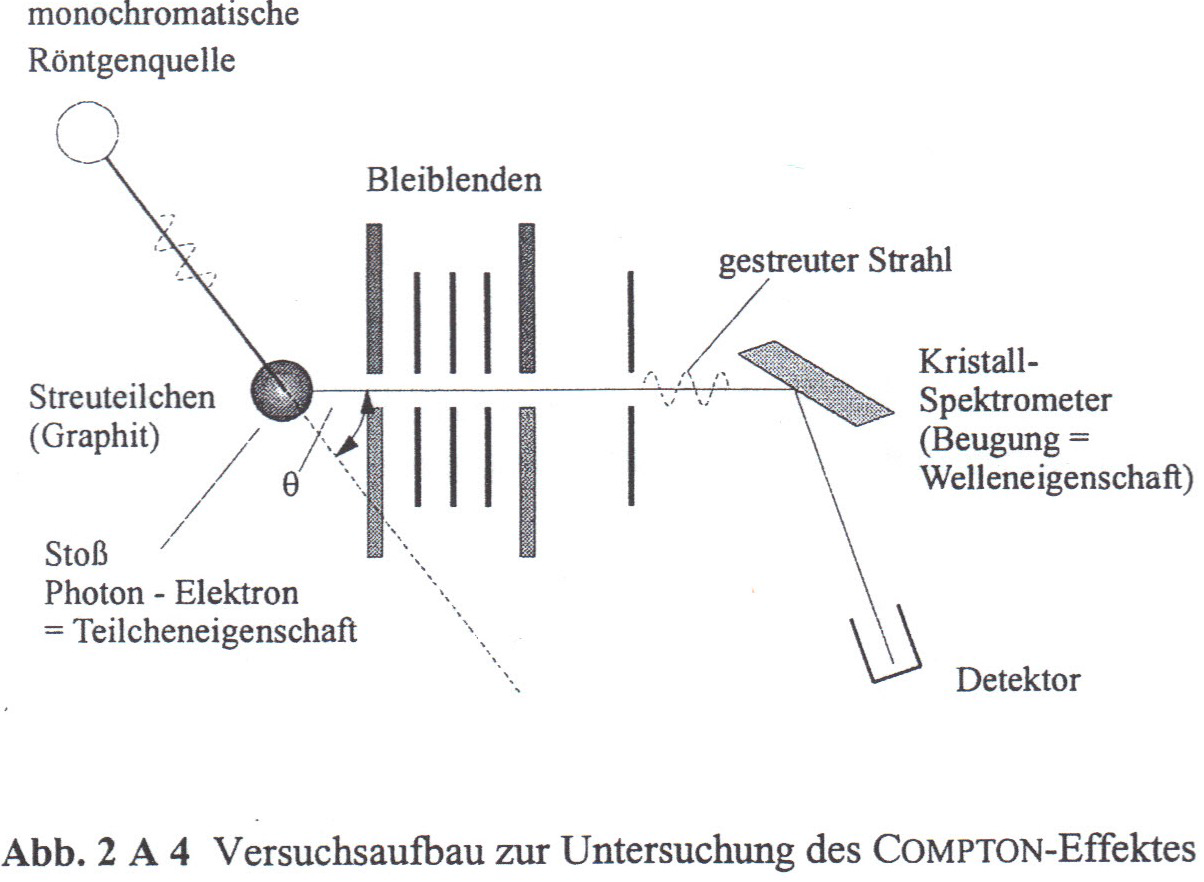
\includegraphics[width=0.5\textwidth]{compton.png} 
\end{center}

Die \textbf{Teilchennatur} zeigt sich bei der Wellenlängenänderung des Streulichts in Abhängigkeit vom Winkel, welche durch (elastische Stöße) der Röntgenphotonen mit den Graphit-Elektronen entstehen. \\ Die \textbf{Wellennatur} zeigt sich bei der Wellenlängenmessung mit dem Kristallspektrometer und dem Detektor, die spektrale Zerlegung ist nur mit der Welleneigenschaft Beugung erklärbar. \\
Wenn die Röntgenphotonen (unelastisch) mit den Atomkernen des Graphits zusammenstoßen, kommt es zu einer Streuung an den Atomen mit unverschobener Wellenlänge. 



\begin{framed}
Bleibt bei einem unelastischen Stoß zweier Körper auf einer waagrechten Ebene die Summe der kinetischen Energien vor dem Stoß erhalten? Welche Erhaltungssätze gelten?
\end{framed}

Die Summe der Kinetischen Energien bleibt nicht erhalten, die Differenzenergie wird zum größten Teil in Wärmeenergie umgewandelt. Ein geringer Teil geht in Verformungsenergie. Gelten tut nur der \textbf{Impulserhaltungssatz}. 



\begin{framed}
Warum liegen beim Natrium-Atom die Energieniveaus mit einer bestimmten Quantenzahlkombination (z.B.: 3S, dh. $n=3,\ell=0$) im Vergleich zum Wasserstoffatom bei viel tieferen Bindungsenergien und andere (z.B.: 3D, dh. $n=3,\ell=2$) bei den selben Energien wie im Wasserstoff-Atom?\\ Wirkt sich derselbe Sachverhalt (und wenn, wie?) bei der Einordnung der chemischen Elemente im Periodensystem aus?
\end{framed}


Die H-Elektronen liegen energetisch günstiger, da die Aufenthaltswahrscheinlichkeit der H-Elektronen ein Nebenmaximum in Kernnähe hat. Dort erfährt das Elektron ein weniger abgeschirmtes COULOMB-Potential des Kerns und ist somit stärker gebunden als ein Na-Elektron. \\
Die physikalischen Merkmale der Atomhülle bestimmen das chemische Verhalten eines Atoms, Atome gleicher Kernladungszahl besitzen dieselbe Atomhülle und sich dadurch chemisch nicht unterscheidbar. Aus der Kernladungszahl erfolgt auch die Einordnung in das Periodensystem. 








\begin{framed}
Mit welchem Modell kann man die Emission von $\alpha$-Teilchen aus dem Atomkern und gleichzeitig die große Variation der Halbwertszeit für $\alpha$-Zerfall erklären?
\end{framed}

Der $\alpha$-Zerfall lässt sich am besten mit dem Tröpfchenmodell erklären, das den Zusammenhang zwischen Energie und Halbwertszeit mittels der GEIGER-NUTTAL-Beziehung angibt, die große Variation kommt durch die Abhängigkeit vom COULOMB-Potential zustande. 










\begin{framed}
Was versteht man unter der transversalen/longitudinalen Modenstruktur und wie kommen diese zustande?
\end{framed}

\begin{itemize}
\item \textbf{Transversale Modenstruktur}: Transversalmoden sind die Abhängigkeit der Intensität der Lichtwellen senkrecht (transversal) zur Ausbreitungsrichtung. Der Abstand der Spiegel eines Resonators muss daher groß gegenüber dem Spiegeldurchmesser sein, Beugungseffekt wird dabei sichtbar. Man kann sich die Spiegel als Reihe von Blenden vorstellen, an jeder wird der Strahl gebeugt. Es zeigt sich, dass die sich einstellenden transversalen Feldmoden mit den transversalen elektromagnetischen Moden identisch sind. 
\item \textbf{Longitudinale Modenstruktur}: Als longitudinal bezeichnet man die Schwingung längs der Ausbreitungsrichtung der Strahlung. Bildlich ausgedrückt handelt es sich dabei um Intensitätsberge und - täler im Abstand einer halben Wellenlänge. Bei einem He-Ne-Laser von einigen Zentimetern Länge könnte man zwischen den Spiegeln etwa 600.000 Intensitätsberge zählen, bei einer kurzen Laserdiode nur einige Tausend. Je nach Bauart werden vom Resonator bestimmte Wellenlängen und deren Vielfache besonders verstärkt, weil sich nur für bestimmte Wellenlängen eine stehende Welle zwischen den Spiegeln ergibt. 
\end{itemize}



\begin{framed}
Beim Helium hat sich gezeigt, dass für gleiche Quantenzahlen $n, \ell$ zwei verschiedene Energiezustände der Elektronen existieren. 
\begin{enumerate}
\item Wodurch kommt dies zustande?
\item Welche Auswirkung hat die hier beobachtete Tatsache letztendlich auf die freien Elektronen in einem Metall?
\item Warum existiert im Triplett-System des Heliums kein Zustand mit Hauptquantenzahl $n=1$?
\item Was ist ein "metastabiler" Zustand der Elektronen des Helium-Atoms?
\item Welche allgemeine Regel resultiert aus dieser Tatsache?
\end{enumerate}
\end{framed}

\begin{enumerate}
\item Helium hat zwei Elektronen und da diese je eine Spin haben, der zwei unterschiedliche Ausrichtungen annehmen kann, gibt es jeden Zustand zweimal. Einmal mit parallelen und einmal mit antiparallelem Spin. Es handelt sich um die einfachen angeregten Zustände des Heliums -  also die, bei denen $n$ und $\ell$ die Quantenzahlen \underline{eines} Elektrons angeben, während das andere stets im Grundzustand $n=1$ und $\ell=0$ ist. 
\item Im Metall liegen Atome auf sehr dichtem Raum zusammen, Die Energieniveaus spalten sich aufgrund der elektrostatischen Wechselwirkung der Elektronen mit unterschiedlichem Spin in 2 Bänder auf, das \textbf{Valenz-} und das \textbf{Leitungsband}. Der Abstand der Bänder ist sehr gering und Elektronen können schon beim Anlegen von sehr kleinen Feldstärken in einen höheren Energiezustand wechseln, sich also "frei bewegen".
\item Hier kommt das PAULI-Prinzip zu tragen, die beiden Elektronen des Heliums müssen sich mindestens in einer Quantenzahl unterscheiden. Triplett bedeutet aber, dass sie denselben Spin haben. Da \underline{ein} Elektron schon im Zustand $n=1,\ell=0$ ist, kann das zweite nur dort Platz nehmen, wenn es sich um einen Singulett-Zustand handelt. 
\item Wegen der Regel $\Delta S = 0$ zerfällt das Energieniveauschema in ein Singulett- und ein Triplett-System, zwischen denen keine optischen Übergänge erlaubt sind, der Übergang zum Grundzustand ist also nicht erlaubt, Atome in diesen Zuständen besitzen relativ lange Lebensdauern, man spricht von "metastabilen" Zuständen. Der Abbau der Besetzungsdichte solcher metastabiler Niveaus kann nur durch (inelastische) Stöße erfolgen.
\item Daraus folgt das PAULI-Prinzip (Zwei Elektronen müssen sich in mindestens einer Quantenzahl voneinander unterscheiden) und die HUNDsche Regel(Tendenz zur maximalen Multiplizität($r=2S+1$)). 
\end{enumerate}

\pagebreak
\begin{framed}
Welche Versuche führten zum RUTHERFORDschen Atommodell?
\end{framed}

RUTHERFORD führte Streuversuche mit $\alpha$-Teilchen an dünnen Goldfolien durch und beobachtete, dass ein Großteil der Teilchen die Folie ungehindert passieren konnte und es nur selten zu einer Ablenkung um einen großen Winkel / Reflexion kam, diese Ablenkungen konnte nur gesteigert werden durch eine Steigerung der Dicke der Folien. \\
Daraus folgerte er, dass die positive Ladung an einer Stelle im Atom konzentriert sein muss (Radius ca $10^{-12}$cm). Dies führte zur Entstehung des Begriffs \textbf{Atomkern}. \\
Um den experimentell bekannten Atomradius zu erklären, ordnete er die Elektronen auf Bahnen weit außerhalb des Kerns an. 



\begin{framed}
Niels Bohr konnte 1913 die Spektralserien des Wasserstoff-Atoms theoretisch deuten, dazu musste er zwei Postulate verwenden, die im Widerspruch zur klassischen Physik stehen, wie lautet diese und in welcher Weise widersprechen sie der klassischen Physik?
\end{framed}

\begin{itemize}
\item Das \textbf{erste Postulat} besagt, dass es bestimmte, stabile Bahnen gibt, auf denen ein Elektron \textbf{strahlungsfrei} umlaufen kann. \\
Die klassische Physik hingegen sieht die Kreisbewegung als eine beschleunigte Bewegung, in der das Elektron elektromagnetische Energie abstrahlen müsste, ergo Energie verlieren müsste und nach geraumer Zeit in den Kern stürzen müsste, es dürften also eigentlich keine stabilen Atome existieren.
\item Das \textbf{zweite Postulat} besagt, dass beim Übergang von einer Bahn höheren Niveaus auf ein niedrigeres Niveau die Energiedifferenz als \textbf{Lichtquant} emittiert wird, umgekehrt diese Energie absorbiert wird, dies erklärt die diskreten Spektren der Atome. \\
Die klassische Physik besagt allerdings, dass die Abstrahlung mit der Umlauffrequenz der Elektronen erfolgen müsste, also kontinuierlich sein müsste. 
\end{itemize}




\begin{framed}
Erklären Sie anhand der radialen Ladungsdichteverteilung der Elektronen, warum nach dem Element Argon zunächst die Elektronen in die 4s-Schale (Kalium) eingebaut werden und nicht in die 3d-Schale?
\end{framed}

\begin{equation*}
\text{Radiale Ladungsdichteverteilung } = R_{n\ell}^{2} \cdot r^2 \cdot e
\end{equation*}
Weil die 4s-Elektronen energetisch günstiger liegen, da die Aufenthaltswahrscheinlichkeit der 4s-Elektronen ein Nebenmaximum in Kernnähe hat. Dort erfährt das Elektron ein weniger abgeschirmtes COULOMB-Potential des Kerns und ist stärker gebunden als ein 3d-Elektron. 

\pagebreak

\begin{framed}
Erklären Sie den Unterschied zwischen spontaner und induzierter Emission.
\end{framed}

\begin{itemize}
\item \textbf{Spontane Emission}: Emission eines Photons (durch Übergang eines Elektrons von einem höheren zu einem niedrigeren Energiezustand) ohne äußere Einwirkung und ohne vorhersehbaren Zeitpunkt.
\item \textbf{Induzierte Emission}: Durch äußere Einwirkung fällt ein Elektron von einem höheren in einen niedrigeren Energiezustand (z.B.: durch Anregung mit einem Photon). Dadurch wird ein Photon emittiert. 
\end{itemize}



\begin{framed}
Wie wird beim Helium-Neon-Laser die Überbesetzung bestimmter Neon-Niveaus erzeugt?
\end{framed}

Durch Gasentladung werden Elektronen des Helium-Atoms auf metastabile Niveaus gehoben, welche sich dann auf gleicher Höhe wie die 3s- und 2s-Niveaus des Neon-Atoms befinden, dabei kann diese Energie dann übertragen werden. Die Elektronen auf den 3s- und 2s-Niveaus des Neons können nun auf 3p- und 2p-Niveaus des Neon-Atoms absinken unter der Emission von Photonen. 


\begin{framed}
\begin{enumerate}
\item Unter welchen Umständen wird von einer bewegten Ladung elektromagnetische Energie abgestrahlt?
\item Woher bezieht diese bewegte Ladung die abgestrahlte Energie?
\end{enumerate}
\end{framed}

\begin{enumerate}
\item Beschleunige elektrische Ladungen strahlen \textbf{während des Beschleunigungsvorgangs} elektromagnetische Wellen (und damit Energie) ab.
\item Aus dem Beschleunigungsvorgang. 
\end{enumerate}



\begin{framed}
Erklären Sie den Zusammenhang zwischen Energie der beim Zerfall radioaktiver Isotope emittierten $\alpha$-Teilchen und der Lebensdauer der zerfallenden Kerne mit Hilfe des Tunneleffekts.
\end{framed}
Ein vom Kern emittiertes $\alpha$-Teilchen müsste klassische eine Energie besitzen, die höher ist als die Potentialbarriere. Als quantenmechanisches Teilchen kann es jedoch mit einer gewissen Wahrscheinlichkeit durch diese Potentialbarriere "durchtunneln" und gelangt dann in das abstoßende COULOMB-Feld des Kerns. Ab dem Abstand $r_0$ überwiegt dann die elektrostatische Abstoßung und das $\alpha$-Teilchen wird auf die Austrittsgeschwindigkeit beschleunigt. Bei größerer Energie des $\alpha$-Teilchens ist die Potentialbarriere schmäler, damit also die Tunnelwahrscheinlichkeit höher und damit auch die Zerfallskonstante $\lambda$ größer und die Halbwertszeit $\tau_H$ kleiner, dadurch die kinetische Energie des emittierten Teilchens höher. \\
Den Zusammenhang zwischen Halbwertszeit und Energie nett man die GEIGER-NUTTAL-Beziehung. 

\pagebreak

\begin{framed}
Wie viele Elektronen können sich in einer voll gefüllten Schale mit Hauptquantenzahl $n$ aufhalten? Warum ist diese Zahl begrenzt?
\end{framed}

Die Anzahl ist begrenzt, da jede Schale nur gewisse Energiezustände zulässt (Elektronen mit gleicher Hauptquantenzahl $n$ fasst man zu einer Schale zusammen). Die Anzahl der möglichen Elektronen in einer Schale ist gegeben durch den Grad der Entartung der Wasserstoff-Energieniveaus $z = 2 \cdot n^2$. 


\begin{framed}
Beschreiben Sie den STERN-GERLACH-Versuch und was wurde mit dessen Hilfe gezeigt?
\end{framed}
In diesem Versuch wurde ein Silberatomstrahl in einem inhomogenen Magnetfeld abgelenkt was klassisch am Auffangschirm einen verwaschenen Fleck ergeben hätte müssen, da jede Einstellung des magnetischen Moments bezüglich der Ag-Atome relativ zum Magnetfeld möglich sein könnte. 
Nach der SOMMERFELDschen Theorie (ohne Spin) hätte sich der Atomstrahlt in 1,3,5... Teilstrahlen aufspalten müssen. \\
Stattdessen wurde eine Aufspaltung des Atomstrahls in nur zwei Teilstrahlen beobachtet, dies führte zur Erkenntnis, dass nur halbzahlige Drehimpulse möglich sind und einen Beweis für den Spin sowie für die Richtungsquantelung. \\
Für das Ag gilt speziell: $L=0, S=1/2$, es ergibt sich also $J = S = 1/2$, daher gibt es nur zwei mögliche Orientierungen in einem äußeren Feld, nämlich $m_j = m_s = \pm 1/2$. 


\begin{framed}
Was versteht man unter dem Unschärfeprinzip von Heisenberg?
\end{framed}
Wenn man Teilchen als ein Wellenpaket auffasst, so gibt es nach der Fourier-Analyse folgende Probleme: \\
Wenn das Wellenpaket aus einer einzigen Frequenz bestehen soll, muss es unendlich ausgedehtn sein, was zu einer Ortsunschärfe führt. \\
Ist das Wellenpaket jedoch in einem Ort $y$ lokalisiert, ist die Frequenz der Welle nicht mehr scharf definiert. \\
Die Unschärfe, die alle Größen betrifft, ist jedenfalls größer als das PLANKsche Wirkungsquantum $h$. \\
Je genauer der Ort eines Teilchens festgelegt wird, desto ungenauer lässt sich sein Impuls bestimmen und umgekehrt. 

\pagebreak

\begin{framed}
Wie wurden die auf einen Elektronenstrahl im magnetischen Feld wirkenden Kräfte demonstriert?
\end{framed}

In einem Fadenstrahlrohr: Ein Elektronenstrahlt wird in einer Glaskugel mit einem geringen Druck eines Gases (z.B.: Neon) erzeugt. Die Glaskugel befindet sich dabei in einem homogen Magnetfeld (HELMHOLTZ-Spulenpaar), das senkrecht zur Bahn der Elektronen wirkt. Die Spur des Elektronenstrahls kann man sehen, weil die Elektronen auf ihrem Weg Gasatome ionisieren und zum Leuchten bringen. Die Ionen stabilisieren den Elektronenstrahl und es bildet sich ein gut gebündelter Fadenstrahl aus. \\
Die Geschwindigkeit der Elektronen ergibt sich aus der Beschleunigungsspannung $U_0$
\begin{equation*}
v = \sqrt{\frac{2 e \cdot U_0}{m}}
\end{equation*}
Die Elektronen erfahren die LORENTZ-Kraft $F_L$ und bewegen sich auf einer Kreisbahn mit dem Radius $R$. Die Zentrifugalkraft $F_Z$ muss gleich groß wie $F_L$ sein. 
\begin{equation*}
F_L = e \cdot v \cdot B = F_Z = \frac{m_e \cdot v^2}{R}
\end{equation*}
\begin{equation*}
\frac{e}{m} = \frac{2 \cdot U_0}{B^2R^2}
\end{equation*}
$B$ und $R$ sind bekannt, bei bekannter Elementarladung kann auch die Masse eines Elektrons ermittelt werden. 


\begin{framed}
Welche Kräfte wirken
\begin{enumerate}
\item auf einen magnetischen Dipol in einem homogenen Magnetfeld?
\item auf einen magnetischen Dipol in einem inhomogenen Magnetfeld?
\item auf einen elektrischen Dipol in einem inhomogenen elektrischen Feld?
\end{enumerate}
\end{framed}

\begin{enumerate}
\item Das magnetische Feld übt die LORENTZ-Kraft auf bewegte Ladungen aus, diese wirkt senkrecht zu den Feldlinien des Magnetfelds sowie senkrecht zur Bewegungsrichtung der Ladung, es wirkt das resultierende Drehmoment
\begin{equation*}
\vec{D} = \vec{p_m}\times \vec{B}
\end{equation*}
\item Resultierende Kraft in eine Richtung, weil die Feldlinien bei einem Pol dichter, also die wirkende Feldstärke größer ist
\begin{equation*}
\vec{F} = \vec{p_m} \cdot grad \ \vec{B}
\end{equation*}
\item Der Dipol wird immer in Richtung der wachsenden Feldstärke gezogen, es wirkt zusätzlich eine Kraft
\begin{equation*}
\vec{F} = \vec{p_el} \cdot \nabla \vec{E}
\end{equation*}
\end{enumerate}

\pagebreak


\begin{framed}
\begin{enumerate}
\item Welche Eigenschaft der Atome wurde mit dem FRANCK-HERTZ-Versuch nachgewiesen?
\item Beschreiben Sie die Versuchsanordnung und den erhaltenen Zusammenhang Strom/Spannung. Gehen Sie auch darauf ein, welche Art von Stößen unter welchen Bedingungen auftreten.
\end{enumerate}
\end{framed}

\begin{enumerate}
\item Der FRANCK-HERTZ-Versuch ist der erste, nicht spektroskopische Nachweis von diskreten Energieniveaus in der Atomhülle. 
\item In einer mit Quecksilberdampf gefüllten Röhre befinden sich eine Kathode und eine Gegenkathode, zwischen welchen eine variable Spannung angelegt wird. Die Kathode wird geheizt, wobei Elektronen austreten und durch die Spannung gegenüber der Gegenkathode beschleunigt werden. Auf ihrem Weg treffen sie mit Atomrümpfen der Quecksilberatome zusammen und regen diese an, wenn sie genügend Energie besitzen. \\
Die Elektronen treten durch die als Gitter ausgeführte Gegenkathode und laufen dort mit ihrer, nach dem Stoß übrig gebliebenen, kinetischen Energie gegen eine Gegenspannung der Anode an und verursachen damit einen Strom. Dieser kann nun in Abhängigkeit von der Kathoden-Gegenspannung gemessen werden und dabei zeigt sich, dass bei steigender Spannung der Strom ebenfalls steigt. \\
Ab einer bestimmten Energie kommt es anstatt von elastischen zu unelastischen Stößen, das Elektron gibt einen Teil seiner Energie an das Hg-Atom ab und regt eines seiner Elektronen an, danach hat das Elektron eine geringere kinetische Energie, kann nicht mehr so stark gegen die Gegenspannung anlaufen und der Strom sinkt. Bei weiterer Spannungserhöhung steigt der Strom wieder, fällt aber, wenn ein Elektron auf seinem Weg mehrere Atome anregen kann usw. \\
Durch Messung der Spannungsdifferenz zwischen den Maxima (bzw. Minima) des Stroms kann man die Anregungsenergie eines Hg-Atoms bestimmen, und zwar 4.9 MeV. \\
\end{enumerate}

\begin{center}
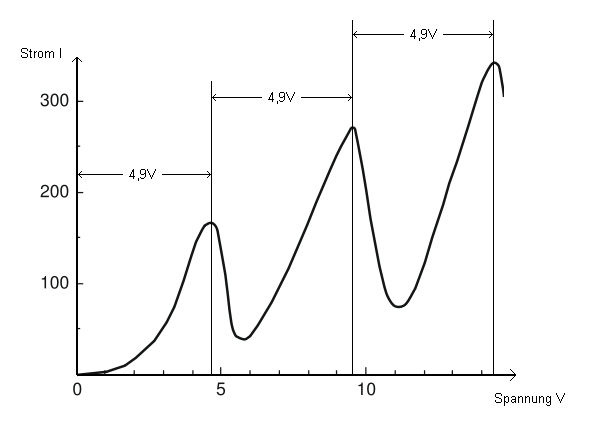
\includegraphics[width=0.53\textwidth]{franckhertz.jpg} 
\end{center}

\pagebreak


\begin{framed}
Wodruch kommt der HALL-Effekt zustande und zur Messung welcher physikalischen Größe wird er verwendet?
\end{framed}
Die auf die Ladungsträger wirkende LORENTZ-Kraft verursacht eine Ablenkung senkrecht zur Fließrichtung des Stroms und senkrecht zum magnetischen Feld. Dadurch baut sich zwischen den Berandungen des Leiters eine HALL-Spannung $U_H$ auf. Die Kraft auf die Ladungsträger im zugehörigen elektrischen Feld $E_H$ kompensiert die LORENTZ-Kraft
\begin{equation*}
U_H = \int{\vec{E_H}\cdot d\vec{s}}
\end{equation*}

Für einen Leiter der Dicke $d$ erhält man für die HALL-Spannung $U_H$
\begin{equation*}
U_H = \frac{I \cdot B}{n \cdot e \cdot d}
\end{equation*}
Somit lässt sich dieser Effekt zur \textbf{Magnetfeldmessung} (Hallsonde) einsetzen. 



\begin{framed}
Welches Gesetz beschreibt die Kraft zwischen zwei Ladungen und wie kann dieses interpretiert werden?
\end{framed}

Das COULOMB-Gesetz lautet
\begin{equation*}
\vec{F} = \frac{1}{4 \pi \epsilon_0}\frac{Q_1 \cdot Q_2}{r^2}\vec{r_e}
\end{equation*}

Für gleichnamige Ladungen wirkt die Kraft also abstoßend, ungleichnamige Ladungen ziehen sich an. Die Kraft nimmt mit dem Abstand quadratisch ab. 



\begin{framed}
Welche Energie muss ein Photon mindestens besitzen, damit es sich in Anwesenheit eines Atomkerns in ein Elektron und ein Positron verwandeln kann?
\end{framed}
\begin{equation*}
E_{min} = h \cdot \nu_{min} = 2 \cdot m_e \cdot c^2
\end{equation*}



\begin{framed}
Welcher grundlegende Unterschied besteht hinsichtlich des Verlaufs der Kraftlinien zwischen einem statischen elektrischen Feld und einem statischen magnetischen Feld, das durch Stromfluss durch einen geraden Leiter aufgebaut wird?
\end{framed}
Das elektrostatische Feld ist ein wirbelfreies Quellenfeld, während das mangetische Feld in quellenfreies Wirbelfeld ist. 

\pagebreak


\begin{framed}
\begin{enumerate}
\item Diskutieren Sie die möglichen Energiezustände und die Aufenthaltswahrscheinlichkeit eines harmonischen Oszillators aus klassischer und quantenmechanischer Sicht!
\item Mit welcher Gleichung wird das Problem in der Quantenmechanik behandelt?
\end{enumerate}
\end{framed}

\begin{enumerate}
\item \textbf{Klassisch} ist jede beliebige Gesamtenergie erlaubt, die Nullpunktenergie ist Null und die Aufenthaltswahrscheinlichkeit zum Rand hin steigt stetig an. Außerhalb des Umkehrpunktes ist diese Null. \\
\textbf{Quantenmechanisch} gibt es eine Quantelung der Energie, es sind also nur diskrete Energiestufen erlaubt, die Nullpunktsenergie ist definiert als
\begin{equation*}
E_0 = \frac{h\cdot \nu}{2}
\end{equation*}

Die Aufenthaltswahrscheinlichkeit oszilliert für $\nu \geq 1$ und klingt außerhalb der klassischen Umkehrpunkte ab. 

\begin{center}
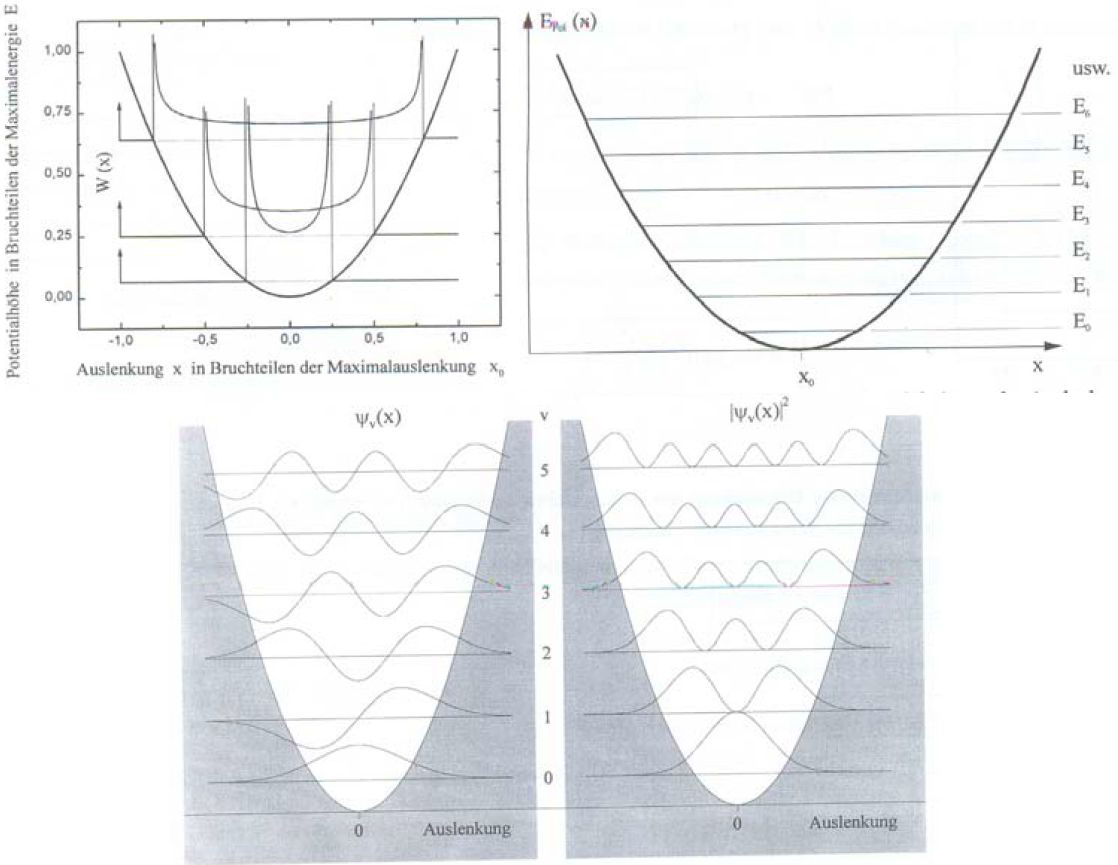
\includegraphics[width=0.5\textwidth]{oszillator.png} 
\end{center}

\item Mit der SCHRÖDINGER-Gleichung, bei der die potentielle Energie $U(x)$ eingesetzt wird
\begin{align*}
-\frac{\hbar^2}{2m} \Delta \Psi - (e-U_{(x,y,z)})\Psi &= 0 \\
E_{pot} = U  &= \frac{k \cdot x^2}{2} \\
-\frac{\hbar^2}{2m}\frac{d^2\Psi(x)}{dx^2} + \frac{1}{2}kx^2\Psi_{(x)} &= E\Psi_{(x)}
\end{align*}
$m$ ist die Masse des Teilchens, $\hbar = \frac{h}{2\pi}$, $\Psi$ ist die zeitfreie Wellenfunktion, $E$ ist die Gesamtenergie, $x$ ist die Auslenkung und $U_{(x,y,z)} = E_{pot}$ ist die Energie in Abhängigkeit der Ortskoordinaten. 
\end{enumerate}

\pagebreak

\begin{framed}
Beim $\beta$-Zerfall wurde beobachtet, dass das emittierte Elektron keine diskrete, sondern eine sich über einen gewissen Bereich erstreckende Verteilung der kinetischen Energie besitzt. Wie wurde der Energiesatz "gerettet"?
\end{framed}
Es wurde angenommen, dass noch ein weiteres Teilchen emittiert wird, welches in der Nebelkammer allerdings nicht sichtbar wurde. Daher wurde diesem Teilchen die Ruhemasse Null und die Ladung 0 zugewiesen und die Existenz dieses "Neutrinos" postuliert, was zu einem späteren Zeitpunkt auch theoretisch und experimentell nachgewiesen werden konnte. 



\begin{framed}
Warum müssen die in einem Reaktor durch Kernspaltung erzeugten Neutronen durch einen Moderator "thermalisiert" werden, damit die Kettenreaktion mit Uran$^{235}$ aufrecht bleibt?
\end{framed}

Je langsamer ein Neutron ist, desto wahrscheinlicher wird es vom Uran aufgenommen und somit die Möglichkeit für eine neue Kernspaltung gegeben. Die Neutronen müssen deshalb auf "thermische" Energien herab gebremst werden. 

\begin{framed}
Welche Eigenschaften muss ein Moderatormaterial besitzen?
\end{framed}
Die Neutronen sollen zwar durch inelastische Stöße abgebremst werden, aber dürfen nicht an den Kern des Moderatoratoms kommen. Die Energieabgabe soll möglichst groß sein, es müssen also viele Atome vorhanden sein. Man braucht also Stoffe mit leichten Kerne, aber hoher Materialdichte z.B.: Graphit oder schweres Wasser. 


\begin{framed}
Wieso erscheint der wolkenlose Himmel blau und wie ist das Morgen/Abendrot zu erklären?
\end{framed}
Da die Flussdichte S des gestreuten Lichts frequenzabhängig ist, kommt es dazu, dass das blaue Licht stärker gestreut wird als das rote Licht, was morgens oder abends dazu führt, das der Himmel rötlich erscheint, da das Licht aufgrund des schrägeren Einfallswinkels einen längeren Weg durch die Atmosphäre hat und dabei das blaue Licht stärker gestreut wird. 

\pagebreak

\begin{framed}
\begin{enumerate}
\item Welche beiden Voraussetzungen müssen erfüllt sein, damit Laserlicht abgestrahlt werden kann?
\item Wie kommt beim He-Ne-Laser die Besetzungsinversion zustande?
\item Was versteht man unter der Kohärenzlänge von Licht? Wie kann diese mit einem Interferometer bestimmt werden und wie hängt diese mit der Frequenzbreite des Lichtes zusammen?
\end{enumerate}
\end{framed}

\begin{enumerate}
\item Besetzungsinversion und eine höhere Wahrscheinlichkeit für induzierte Emission im Vergleich zu spontaner Emission. letztere wird durch den Resonator erzeugt. Die dadurch zustande kommenden Moden müssen im verstärkenden Bereich des aktiven Mediums und oberhalb der Laserschwelle liegen.
\item Die oberen Laserlinien-Niveaus werden durch Stöße mit metastabilen He-Atomen selektiv besetzt, wodurch zwischen den Niveaugruppen eine Besetzungsinversion entsteht. 
\item Hier muss man zuerst die \textbf{Kohärenzzeit} definieren, dass ist jene Zeit $\Delta t$, in der die Welle mit unveränderter Phase schwingt. 
Der Wellenzug ist eine Überlagerung von verschiedenen Teilwellen, die auf der Kohärenzlänge konstruktiv, darüber hinaus destruktiv interferieren. Die Kohärenzlänge ist von der Anzahl der vorkommenden Frequenzen abhängig, je mehr vorkommen, desto kürzer ist die Kohärenzlänge. Interferenz kann zum Beispiel nur beobachtet werden, wenn der optische Wegunterschied kleiner als die Kohärenzlänge ist, darum kann man Farbeffekte bei weißem Licht auch nur bei sehr dünnen Schichten beobachten. 
Die Kohärenzlänge ist definiert als
\begin{equation*}
 \ell = c \cdot \Delta t = \frac{c}{\delta \nu}
 \end{equation*} 
 
\begin{center}
 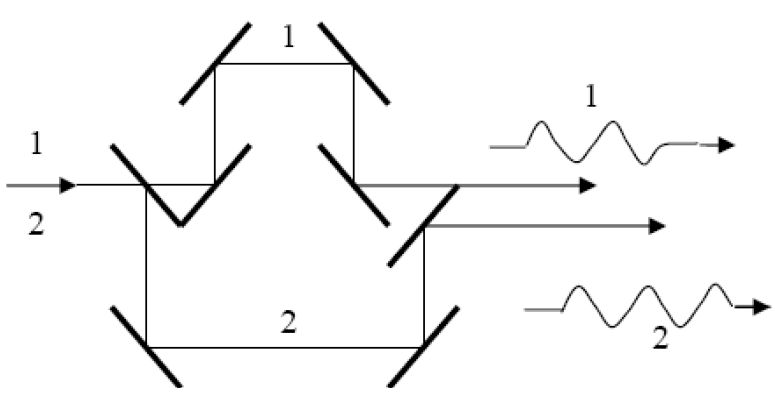
\includegraphics[width = 0.5\textwidth]{interferometer.png} 
\end{center}
 
 Interferenz von Teilstrahl 1 und 2 ist nur dann möglich, wenn gilt \begin{equation*}
 \ell_2 - \ell_1 < \ell_c
 \end{equation*}
\end{enumerate}


\pagebreak

\begin{framed}
\begin{enumerate}
\item Geben Sie die beiden besprochenen Modelle für den Aufbau der Atomkerne an und geben Sie an, was für das jeweilige Modell spricht.
\item Wie konnten Neutronen erzeugt und nachgewiesen werden?
\end{enumerate}
\end{framed}

\begin{enumerate}
\item \textbf{Tröpchenmodell}: Dieses Modell beschreibt die Analogie des Kerns zu einem \\ Flüssigkeitstropfen und erklärt damit die konstante, von der Massenzahl weitgehend unabhängige, Dichte, die geringe Reichweite der Kernkräfte und die konstante Bindungs-energie pro Nukleon. Aus dieser Beschreibung kann man ableiten, dass leichte Atomkerne durch Fusion Energie freigeben und schwere Atomkerne durch Kernspaltung. \\
\textbf{Schalenmodell}: Ordnet Neutronen und Protonen selbst wie auf Schalen an, der Kern ist somit wie die Hülle aufgebaut (es gilt auch das PAULI-Prinzip, es gibt Spins für Nukleonen...). Dadurch werden Effekte wie Kernspin, magnetisches Moment, elektrisches Quadrupolmoment und $\beta$-Strahlung erklärt. Auch das Vorkommen "magischer Zahlen", also Neutronen- und Protonenzahl, die besonders stabile, isotopenfreundlichen Kerne kennzeichnet, wird dadurch erklärt. 
\item Es gibt mehrere Arten von Neutronenquellen, einerseits die \textbf{Kernreaktion mit Neutronen-Abgabe}, dann \textbf{Fusionsneutronenquellen}, die hauptsächliche Quelle für langsame Neutronen sind \textbf{Kernreaktoren}, \textbf{Photonenneutronenquellen} und beim "Zerschlagen" von Deuterium werden Neutronen abgegeben. \\
Entdeckt wurde das Neutron von CHADWICK nach Experimenten von Marie CURIE aus der Kernreaktion $_4Be^9(\alpha,n) _6C^{12}$(durch Mischung von Radiumchlorid als Lieferant von $\alpha$-Teilchen und Be-Pulver, bei dieser Kernreaktion werden ein \textbf{Neutron n} und ein $\gamma$-Quant emittiert).
\end{enumerate}


\begin{framed}
Welche Anforderungen stellt man an eine Lichtleitfaser zur Nachrichtenübertragung und nach welchen Gesichtspunkten wird man die Wellenlänge des Lichts, mit dem Informationen übertragen werden, auswählen?
\end{framed}

Die Lichtleitfaser soll eine möglichst \textbf{kleine Dispersion} und eine \textbf{geringe Dämpfung} aufweisen. Die Wellenlänge des Lichts wird in Abhängigkeit des Leichtleiterdurchmessers gewählt. Bei falscher Wahl kommt es zu "Zerfließen" des Signals infolge von Dispersion. 


\pagebreak


\begin{framed}
Wie wurde von EINSTEIN der lichtelektrische (photoelektrische) Effekt gedeutet und welche Folgerungen ergeben sich daraus?
\end{framed}

Ultraviolettes Licht trifft auf eine Elektrode und löst dort Elektronen aus, die vom Licht bereitgestellte Energie muss dabei die Elektronen aus der Metalloberfläche befreien. Die nicht verbrauchte Energie wird in Form von kinetischer Energie aufgenommen. Diese kann gemessen werden, indem man die Elektronen gegen ein Potential anlaufen lässt. Wenn man die Spannung so einstellt, dass der Strom Null wird, kann man die kinetische Energie der Elektronen bestimmen, sie ist die Restenergie, die übrig bleibt, nachdem das Photon die Ablösearbeit W erbracht hat, es gilt dabei
\begin{equation*}
h \cdot \nu = \frac{m_ev^2}{2} + W
\end{equation*}
Dabei ist die Stromstärke von der Intensität der Strahlung, die Spannung von der Wellenlänge der Strahlung abhängig. \\
EINSTEIN deutete dies als einen \textbf{unelastischen Stoß} zwischen Photon und Elektron, bei dem Energie übertragen wird. \\
Die Folgerungen waren
\begin{itemize}
\item \textbf{Lichtquanten} besitzen diskrete Energie
\item Energie wird vollständig auf Elektronen übertragen
\item Anzahl der ausgelösten Elektronen ist unabhängig von der Wellenlänge, aber proportional zur Intensität der Strahlung
\item Lichtquant verhält sich wie ein stoßendes Teilchen - Rückkehr zum \textbf{Korpuskelbild} des Lichts
\end{itemize}


\begin{framed}
Was versteht man unter einer "Hystereseschleife"?
\end{framed}
Die Hystereseschleife beschreibt den nichtlinearen Verlauf der Magnetisierung von ferromagnetischen Stoffen (Abhängigkeit der Flussdichte $\vec{B}$ von der magnetischen Erregung $\vec{H}$), dabei spielt natürlich die Vorgeschichte des Materials eine große Rolle. Erhöht man die magnetische Erregung, steigt die Flusdichte, bis sie irgendwann in Sättigung geht, senkt man die Erregung wiederum auf Null, so bleibt eine gewisse "Remanenzinduktion" übrig. Die magnetische Erregung, die dann notwendig ist, um die Induktion auf Null zu bringen, nennt man Koerzitiverregung. Bei einer breiten Schleife spricht man von hartmagnetischen Stoffen, bei einer schmalen Schleife von weichmagnetischen Stoffen. 















\pagebreak
\section*{Rechenfragen}


\begin{framed}
Ein Linsensystem besteht aus einer Zerstreuungslinse ($f=-10cm$) und einer Sammellinse ($f=12cm$) im Abstand von 9 cm. Der Gegenstand wird 8 cm vor der Zerstreuungslinse angeordnet.
\begin{enumerate}
\item In welcher Entfernung von der Sammellinse entsteht das Bild? Wie groß ist der Abbildungsmaßstab?
\item Wie groß muss die Brennweite einer Ersatzlinse sein, und wo muss sie aufgestellt werden, damit das Bild am selben Ort und mit der selben Größe entsteht?
\end{enumerate}
\end{framed}

\begin{enumerate}
\item \begin{align*}
f_Z = -10cm, \ f_S = 12cm, \ g_1 = 8cm \\
\end{align*}
Die allgemeine Formel lautet nun in im ersten Fall
\begin{align*}
\frac{1}{f_Z} = \frac{1}{g_1} + \frac{1}{b_1} \\
b_1 = \frac{1}{\frac{1}{f_z}-\frac{1}{g_1}} = \frac{1}{\frac{1}{-10}-\frac{1}{8}} &= -4.44 cm \\
g_2 = 9cm - b_1 &= 13.44cm \\
b_2 = \frac{1}{\frac{1}{f_s}-\frac{1}{g_2}} = \frac{1}{\frac{1}{12} - \frac{1}{13.44}} &= \underline{111.69cm}
\end{align*}
Damit ergibt sich für den Abbildungsmaßstab
\begin{align*}
M = \left(-\frac{b_1}{g_1}\right) \cdot \left(-\frac{b_2}{g_2}\right) = \frac{-4.44}{8} \cdot \frac{111.69}{13.44} = -4.615
\end{align*}
Es entsteht also ein verkehrtes, vierfach vergrößertes Bild. 
\item Der gesamte Abstand zwischen Gegenstand und Abbildung ergibt sich aus der gesamten Distanz zwischen Gegenstand - Linse 1 - Linse 2 - Abbildung
\begin{align*}
|b| + |g| = 8 + 9 + 111.69 = 128.69cm
\end{align*}
Mit dem bisher bekannten Abbildungsmaßstab von $-4,615$ gilt nun
\begin{align*}
M = -\frac{b}{g} = -4.615 \Rightarrow -b = -4.615 \cdot g
\end{align*}
Damit ergibt sich für die Gegenstandsweite
\begin{align*}
M_T = -4.615 &= -\frac{\text{Gesamtdistanz - Gegenstandsweite g}}{g} \\ &=\frac{128.69-g}{g} = -\frac{128.69}{g} + \frac{g}{g} = \frac{128.69}{g} +1 \\  &\Rightarrow 5.615g = 128.69
\end{align*}
Damit folgt daraus $g=22.92cm$ und $b=128.69-g=105.77cm$. Damit lässt sich die Brennweite berechnen zu
\begin{align*}
f = \frac{1}{\frac{1}{g}+\frac{1}{b}} = \frac{1}{\frac{1}{22.92} + \frac{1}{105.77}} = 18.84 cm
\end{align*}
\end{enumerate}


\begin{framed}
 Eine Sammellinse bildet einen Gegenstand 4-fach vergrößert reell ab, verschiebt man die Linse gegenüber dem Gegenstand um 1cm, so erhält man ein 5-fach vergrößertes, ebenfalls reelles Bild. Wie groß ist die Brennweite der Sammellinse?
\end{framed}

Damit man eine größere Vergrößerung erhält, muss man die Linse zum Gegenstand bewegen. Dadurch kann man auf die beiden Abbildungsmaßstäbe schließen
\begin{align*}
M_T &=-\frac{b}{g} = -4 \\
M_T &= -\frac{b_1}{g-1} = -5 \\
\frac{1}{f} = \frac{1}{b}+\frac{1}{g} &= \frac{1}{b_1}+\frac{1}{g-1} = \frac{1}{f}
\end{align*}
Nun kann man die Gleichungen umgeformen $b = 4g$ und $b_1 = 5(g-1)$  einsetzen
\begin{align*}
\Rightarrow \frac{1}{4g} + \frac{1}{g} &= \frac{1}{5(g-1)} + \frac{1}{g-1} \\
\frac{1+4}{4g} &= \frac{1+5}{5g-5} \\
\frac{5}{4g} &= \frac{6}{5g-5} \\
25g-25 &= 24g \Rightarrow g = 25 \\
b &= 100
\end{align*}
Daraus wiederum lässt sich die Brennweite der Linse berechnen
\begin{align*}
\frac{1}{f} = \frac{1}{25} + \frac{1}{100} \Rightarrow f = 20cm
\end{align*}

\pagebreak


\begin{framed}
\begin{enumerate}
\item An eine Röntgenröhre wird eine Spannung von $U = 50kV$ angelegt. Wie groß ist die Mindestwellenlänge $\lambda_{min}$ der emittierten Röntgenstrahlung? Warum tritt keine Strahlung mit $\lambda < \lambda_{min}$ auf? Skizze der spektralen Röntgen-Bremsstrahlung.
\item Unter welchen Winkeln würde man Beugungsmaxima beobachten, wenn man als Wellenlänge das 2.5-fache der in 1.) berechneten Mindestwellenlänge annimmt (Kristallspektrometer mit $d = 1 \mathrm{\AA}$). Einige Winkel und Beugungsordnungen angeben.
\item Wie groß muss die Kernladungszahl der Antikathode mindestens sein, damit bei $50kV$ noch keine charakteristische Röntgenstrahlung auftritt (Ionisierungsenergie des Wasserstoffatoms = 13.6eV)?
\item Schätzen Sie ab, ob bei der benutzen Röntgenröhre bereits charakteristische Strahlung auftritt, wenn die Antikathode aus Wolfram gefertigt wurde (Ionisierungsenergie des Wasserstoffatoms 13.6eV, Kernladungszahl von Wolfram Z = 74).
\item Berechnen Sie aus der Ionisierungsenergie des Wasserstoffatoms den Abstand des Elektrons vom Kern.
\item Strahlung mit $\lambda_{min}$ trifft auf einen Kristall mit einem Gitterebenenabstand von $1 \mathrm{AA}$. Unter welchem Einfallswinkel wird BRAGGsche Reflexion beobachtet?
\end{enumerate}
\end{framed}
\begin{enumerate}
\item
Genutzt wird hierbei die Formel $U \cdot e = h \cdot \nu$ und der Zusammenhang $\nu = \frac{c}{\lambda}$:
 \begin{align*}
U = 50kV \\
U \cdot e = h \cdot \nu_{max} = \frac{h \cdot c}{\lambda_{min}}
\end{align*}
Nach Umformung erhält man dann
\begin{align*}
\lambda_{min} = \frac{h \cdot c}{U \cdot e} = \frac{6.62\cdot 10^{-34} Js \cdot 3 \cdot 10^8m/s}{50\cdot 10^3V \cdot 1.602 \cdot 10^{-19}C} = 2.48\cdot 10^{-11} m = 0.248 \mathring{A}
\end{align*}
(1 \AA ngström = $10^{-10}$m). \\
Die Formel $U \cdot e = h \cdot \nu_{max}$ gilt \textbf{nur} dann, wenn die gesamte kinetische Energie des Elektrons in Strahlung umgewandelt wird. Da aber nur ein Teil dieser Energie umgewandelt wird, können nur kleinere Frequenzen = größere Wellenlängen vorkommen. Je kleiner die Wellenlänge, desto höher die Energie. 
\pagebreak
\\
Die dazugehörige Skizze
\begin{center}
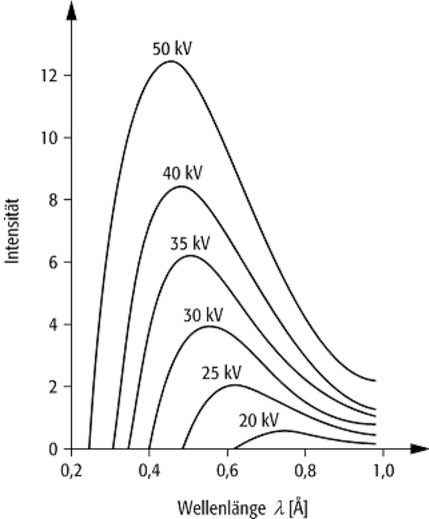
\includegraphics[width=0.3\textwidth]{roentgen.png} 
\end{center}


\item BRAGGsche Reflexionsbedingung, hierbei gilt
\begin{equation*}
\Delta s = k \cdot \lambda = 2 \cdot d \cdot sin(\varphi) \text{ ... BRAGGsche Reflexionsbedingung}
\end{equation*}
\begin{equation*}
\lambda = \lambda_{min} \cdot 2.5 = 0.62 \AA
\end{equation*}
\begin{equation*}
sin(\varphi) = \frac{k \cdot \lambda}{2 \cdot d} \Rightarrow \varphi = sin^{-1}\left(\frac{k \cdot \lambda}{2 \cdot d}\right)
\end{equation*}
Die Winkel sind bei den ersten drei Beugungsmaxima zu erkennen bei
\begin{equation*}
k=1: \varphi_1 = sin^{-1}\left(\frac{1 \cdot 0.62\AA}{2 \cdot 1\AA}\right) = 0.315 = 18.06^\circ
\end{equation*}
\begin{equation*}
k=2: \varphi_2 = sin^{-1}\left(\frac{2 \cdot 0.62\AA}{2 \cdot 1\AA}\right) = 0.669 = 38.32^\circ
\end{equation*}
\begin{equation*}
k=3: \varphi_3 = sin^{-1}\left(\frac{3 \cdot 0.62\AA}{2 \cdot 1\AA}\right) = 1.194 = 68.43^\circ
\end{equation*}
\item
\begin{align*}
U_{min} &= \frac{13.6 \cdot 1.602\cdot 10^{-19}J \cdot Z^2}{e} > 50kV \\
Z^2 &> \frac{50kV \cdot 1.602\cdot 10^{-19}C}{13.6 \cdot 1.602 \cdot 10^{-19}J} \\
Z &> \sqrt{3676.5} = 60.63 \approx 61
\end{align*}
Die Kernladungszahl muss also $\geq 61$ sein, damit keine charakteristische Röntgenstrahlung auftritt. 
\pagebreak
\item 
\begin{align*}
E_{min} = e \cdot U_{min} = R_x(Z-\sigma)^2 \frac{1}{n^{'2}} \\
\text{mit } n^{'} \text{ und } \sigma \approx 1 \text{ nun } U_{min} \text{ berechnen: } \\
U_{min} = \frac{13.6 \cdot e \cdot 73^2}{e} = 72.474kV
\end{align*}
Für $U<U_{min}$ tritt somit keine charakteristische Strahlung auf!

\end{enumerate}

\begin{framed}
Die Rydbergkonstante für das Wasserstoffatom beträgt $109677cm^{-1}$. 
\begin{enumerate}
\item Wie groß ist die Wellenlänge der Balmer-Linie$H_\alpha$ (Übergang n = 5 zu n = 2) und der Lyman-Linie $L_\alpha$ (Übergang n=2 zu n=1)?
\item Wie groß ist die Ionisierungsenergie des Wasserstoffatoms (in eV, Berechnung aus der gegebenen Rydbergkonstante)?
\end{enumerate}
\end{framed}
\begin{enumerate}
\item Balmer-Linie $H_\alpha$:
\begin{align*}
f = R_H\cdot \left(\frac{1}{2^2} - \frac{1}{n^2}\right) &= 10967700m^{-1} \cdot \left(\frac{1}{2^2} - \frac{1}{5^2}\right) = 2303217m^{-1} \\
\lambda = \frac{1}{f} &= \frac{1}{2303217m1{-1}} = 434,18nm
\end{align*}
Lyman-Linie $L_\alpha$:
\begin{align*}
f = R_H\cdot \left(\frac{1}{1^2} - \frac{1}{n^2}\right) &= 10967700m^{-1} \cdot \left(\frac{1}{1^2} - \frac{1}{2^2}\right) = 8225775m^{-1} \\
\lambda = \frac{1}{f} &= \frac{1}{8225775m1{-1}} = 121.57nm
\end{align*}
\item \begin{align*}
E_{ion} \cdot \frac{1}{n^2} &= -h \cdot c \cdot R_H \cdot \frac{1}{n^2} \\
E_{ion} &= h \cdot c \cdot R_H = 6.62 \cdot 10^{-34}Js \cdot 3 \cdot 10^8m/s \cdot 10967700m^{-1} = 217818522 \cdot 10^{-26}J \\
1eV &... 1.602 \cdot 10^{-19}J \Rightarrow \frac{217818522 \cdot 10^{-26}J}{1.602 \cdot 10^{-19}J} \cdot 1eV = 13.5967eV
\end{align*}
\end{enumerate}

\pagebreak

\begin{framed}
Ein Körper (m=1kg) kann reibungsfrei auf einer parabelförmigen Bahn gleiten. Sein Mittelpunkt befindet sich 2m über dem Bahnminimum. Die Bahnform ist symmetrisch um den Nullpunkt und gehorcht der Gleichung $h(x) = b \cdot x^2$ mit $b = 2m^{-1}$. 
\begin{enumerate}
\item Wie groß ist die Geschwindigkeit auf halber Höhe und auf Höhe Null?
\item Wie hängt die auf den Körper wirkende Kraftkomponente in Richtung der x-Achse von der Auslenkung x ab (Gleichung für F(x) herleiten)?
\item Welche Größe bleibt während der gesamten Bewegung erhalten und welche Bewegung wird er ausführen?
\item Geben Sie die Gleichung für die Beschleunigung $a$ in x-Richtung an!
\end{enumerate}
\end{framed}

\begin{enumerate}
\item Es gilt
\begin{equation*}
E = m \cdot g \cdot h + \frac{m \cdot v^2}{2} \Rightarrow E_{ges.} = m \cdot g \cdot h + 0 = 20 J
\end{equation*}
Auf halber Höhe gilt somit
\begin{equation*}
E_{kin,1m} = E_{ges.}-E_{pot,1m} = 10J = \frac{m \cdot v^2}{2} \Rightarrow v_{1m} =\sqrt{2 \cdot 10 \cdot 1}  = 4.472 \frac{m}{s}
\end{equation*}
Auf Höhe Null gilt dann
\begin{equation*}
E_{kin,0m} = E_{ges.}-E_{pot,0m} = 20J = \frac{m \cdot v^2}{2} \Rightarrow v_{2m} =\sqrt{2 \cdot 20 \cdot 1}  = 6.325 \frac{m}{s}
\end{equation*}
\item Es gilt
\begin{equation*}
W = \int{F \cdot dx} \Rightarrow F_x = \frac{dW}{dx}
\end{equation*}
\begin{equation*}
W = -E_{pot} = -m \cdot V_{pot} = -m\cdot g\cdot h = -m \cdot g \cdot b \cdot x^2
\end{equation*}
\begin{equation*}
F_{(x)} = -\frac{d}{dx}\cdot m \cdot g \cdot b\cdot x^2 = -2mgbx
\end{equation*}
\item Die Energie und die Masse bleiben erhalten. Der Körper führt eine oszillierende Bewegung aus auf der Parabelbahn. 
\item \begin{equation}
F_{x} = m \cdot a(x) \Rightarrow a(x) = \frac{F(x)}{m} = -2gbx
\end{equation}
\end{enumerate}

\pagebreak

\begin{framed}
Das Licht der roten Cd-Linie $644nm$ (Übergang im Singulett-System) wird in einem Magnetfeld von $B = 0.7$ Tesla emittiert. Wie groß ist die Frequenzänderung des emittierten Lichts und wie groß muss das Auflösungsvermögen $\nu /\Delta \nu$ eines optischen Instruments sein, damit der Effekt deutlich beobachtet werden kann? (Aufspaltung = 2x auflösbare Frequenzänderung) ($\mu_B = 9.27 \cdot 10^{-24}J/T$)
\end{framed}

\begin{align*}
\Delta E = \mu_B \cdot B = 9.27 \cdot 10^{-24} \cdot 0.7 = 6.49 \cdot 10^{-24} J \\
\Delta E = h \cdot \Delta \nu \Rightarrow \Delta \nu = 9.8 \cdot 10^9 Hz \\
\end{align*}
Das Gerät muss daher mit mindestens $\Delta \nu /2 = 4.9 \cdot 10^9 Hz$ auflösen. Zur Bestimmung des Auflösungsvermögen muss jetzt noch die Frequenz selbst bestimmt werden
\begin{align*}
\nu = \frac{c}{\lambda} = \frac{c}{0.000000644m} = 4.66 \cdot 10^{14}Hz
\end{align*}
Daraus ergibt sich nun ein Auflösungsvermögen von $\frac{\nu}{\Delta \nu} = 95102$. 

\begin{framed}
Ein gut kollimierter Elektronenstrahl trifft auf einen Kristall mit dem Netzebenenabstand $d = 0.9 \mathrm{\AA}$. Bei $\varphi = 25^\circ$ beobachtet man ein Interferenzmaximum 1.Ordnung (BRAGGsche Reflexion). 
\begin{enumerate}
\item Wie groß ist die DE BROGLIE-Wellenlänge der Elektronen und mit welcher Spannung wurden die Elektronen beschleunigt?
\item Derselbe Kristall zeigt für monochromatisches Röntgenlicht unter demselben Winkel ein Reflexionsmaximum. Wie groß muss die Spannung an der Röntgenröhre sein, wenn man annimmt, dass 20\% der Elektronenenergie in Strahlungsenergie umgewandelt wird?
\end{enumerate} 
\end{framed}

\begin{enumerate}
\item \begin{align*}
\Delta s = k \cdot \lambda &= 2 \cdot d \cdot sin \ \varphi = \frac{h}{m \cdot v} \\
\lambda = 0.76707\cdot 10^{-10}m \Rightarrow v &= \frac{h}{m \cdot \lambda} = \frac{6.62 \cdot 10^{-34}}{9.109 \cdot 10^{-31} \cdot 0.76707 \cdot 10^{-10}} = 9.5 \cdot 10^6 \\
U \cdot e = \frac{m \cdot v^2}{2} &\Rightarrow U = \frac{m \cdot v^2}{2 \cdot e} = 259.5 V
\end{align*}
\item \begin{align*}
E = h \cdot \nu = \frac{h \cdot c}{\lambda} = 1.986 \cdot 10^{-15} J \\
n = 20\% \Rightarrow E_e = \frac{E}{n} = 9.923 \cdot 10^{-15}J \\
E_e = e \cdot U \Rightarrow U = \frac{E_e}{e} = 61.94 kV
\end{align*}
\end{enumerate}

\pagebreak

\begin{framed}
Sie führen einen schiefen Wurf durch, der Körper startet mit Geschwindigkeit $v_0$ in waagrechter Richtung und $v_{\bot}$ in vertikaler Richtung nach oben. Geben sie folgende Gleichungen an: $x(t),y(t),y(x)$. Welche geometrische Form hat die Bahnkurve?
\end{framed}
Der schiefe Wurf setzt sich zusammen aus freiem Fall (beschleunigte Bewegung) in senkrechter Richtung und gleichförmiger Bewegung in waagrechter Richtung. 
\begin{align*}
x(t) &= v_0 \cdot t \Rightarrow t = \frac{x(t)}{v_0} \\
y(t) &= v_\bot \cdot t - \frac{1}{2}\cdot g \cdot t^2 \\
y(x) &= v_\bot \cdot \frac{x}{v_0} - \frac{1}{2} \cdot g \cdot \left(\frac{x}{v_0}\right)^2
\end{align*}
Die Wurfbahn folgt einer Parabel. 


\begin{framed}
Die erste künstliche Kernumwandlung wurde mit der Reaktion
\begin{align*}
_7N^{14} + _2He^4 \ \Rightarrow \ _8O^{17} + 1_H^1
\end{align*}
nachgewiesen, die relativen Atommassen sind dabei: \\$_7N^{14}:14.0031; _2He^4:4.0026; _8O^{17}:16.9993; 1_H^1:1.0078$. 
\begin{enumerate}
\item Welche Mindestenergie (in MeV) muss das $\alpha$-Teilchen am Kernort noch besitzen, um die Reaktion auszulösen?
\item Welche Gesamtenergie muss das $\alpha$-Teilchen (im Abstand unendlich) besitzen, um die Reaktion auszulösen (Die Annäherung an den N-Kern soll bis auf $3 \cdot 10^{-13}cm$ notwendig sein)?
\end{enumerate}
\end{framed}

\begin{enumerate}
\item \begin{gather*}
E \geq \Delta m \cdot c^2 \\
\Delta m = m_{Aus} - m_{Ein} = (16.9993+1.0078)-(14.0031+4.0026) = 0.0014u \\
1u = 1.66 \cdot 10^{-27}kg \Rightarrow \Delta m = 0.0014 \cdot 1.66 \cdot 10^{-27}kg = 2.32477 \cdot 10^{-300}kg \\
E_{min} = \Delta m \cdot c^2 = 208.871 \cdot 10^{-15}J = 1.303 MeV
\end{gather*}
\item \begin{gather*}
E_{Ges} = \frac{1}{4 \pi \epsilon_0}\cdot \frac{Z_{Projektil} \cdot Z_{Kern}\cdot e^2}{r} = \frac{1}{4 \pi \epsilon}\frac{1\cdot 40 \cdot e^2}{3\cdot 10^{-15}} = 3.077 \cdot 10^{-12}J = 19.2 MeV
\end{gather*}
\end{enumerate}

\pagebreak

\begin{framed}
Ein Atomkern mit relativer Masse $237.9456$ emittiert ein $\alpha$-Teilchen (relative Masse $4.0026$) der Energie $5MeV$ und der entstandene angeregte Zwischen-Kern anschließend ein $\gamma$-Quant der Energie $1.2MeV$. Wie groß ist die relative Masse des stabilen Endkerns?
\end{framed}

\begin{gather*}
1.2 \cdot 10^6 eV \cdot 1.602 \cdot 10^{-19} = 1.9224 \cdot 10^{-13}J \\
\Delta E = \Delta m \cdot c^2 \Rightarrow \Delta m = \frac{\Delta E}{c^2} = \frac{1.9224 \cdot 10^{-13}J}{(3 \cdot 10^8 \frac{m}{s})^2} = 2.136 \cdot 10^{-30}kg \\
\frac{2.136 \cdot 10^{-30}kg}{1.66055 \cdot 10^{-27}kg} = 0.001287u \\
\Delta m = 237.9456 - 4.0026 - 0.001287 = 233.942u
\end{gather*}


\begin{framed}
Die Elektronen eines Elektronenstrahls werden zunächst mit Hilfe einer Spannung von 200V auf konstante Geschwindigkeit gebracht. Danach durchläuft der Strahlt ein senkrecht zu seiner Richtung angeordnetes, homogenes elektrisches Feld (Abstand der Kondensatorplatten 1cm, Länge 5cm, Kondensatorspannung 10V).
\begin{enumerate}
\item Wie groß ist die Ablenkkraft auf die Elektronen im Kondensator?
\item Welche Geschwindigkeit senkrecht zur ursprünglichen Strahlrichtung besitzen die Elektronen des Strahls nach dem Kondensator?
\item Unter welchem Winkel zur ursprünglichen Richtung verlässt der Strahl den Kondensator?
\end{enumerate}
\end{framed}

\begin{enumerate}
\item \begin{gather*}
F = e \cdot E \\
E = \frac{U}{d} = \frac{10}{0.01} = 1000 \frac{V}{m} \\
F = 1.602 \cdot 10^{-19}\cdot 1000 = 1.602 \cdot 10^{-16}N
\end{gather*}
\item \begin{gather*}
E_{kin} = e \cdot U_0  = \frac{m \cdot v^2}{2} \Rightarrow v_0 = \sqrt{\frac{2 \cdot e \cdot U_0}{m}} = \sqrt{\frac{2 \cdot 1.602 \cdot 10^{-19}\cdot 200}{9.109 \cdot 10^{-31}}} = 8.387 \cdot 10^6 \frac{m}{s} \\
t = \frac{l}{v_0} = \frac{0.05}{8.387 \cdot 10^{-31}} = 5.961 \cdot 10^{-9}s \\
a_{senkrecht} = \frac{F}{m} = \frac{1.602 \cdot 10^{-16}}{9.1 \cdot 10^{-31}} = 1.759 \cdot 10^{14} \frac{m}{s^2} \\
v_{senkrecht} = a_{senkrecht} \cdot t = 1.759 \cdot 10^{14} \cdot 5.961 \cdot 10^{-9} = 1.049 \cdot 10^6 \frac{m}{s}
\end{gather*}
\pagebreak
\item 1. Möglichkeit: 
\begin{gather*}
\Delta Z = \frac{a \cdot t^2}{2} = \frac{1.759 \cdot 10^{14} \cdot 5.961 \cdot 10^{14}}{2} = 0.003126m \\
\alpha = arctan \frac{\Delta Z}{\frac{l}{2}} = arctan \frac{0.3126}{2.5}= 7.13^\circ = 0.124 rad
\end{gather*}
2. Möglichkeit:
\begin{gather*}
\alpha = arctan\frac{v_{senkrecht}}{v_0} = arctan\frac{1.049 \cdot 10^6 \frac{m}{s}}{8.387 \cdot 10^{6}\frac{m}{s}} = 7.13^\circ = 0.124 rad
\end{gather*}
\end{enumerate}


\begin{framed}
Ein He-Ne-Laser emittiert bei $633nm$ eine Lichtleistung von $2mW$.
\begin{enumerate}
\item Wie hoch sind der Photonenfluss (Photonen/s) und die Energiedichte (Strahlquerschnitt $2mm^2$; $h = 6.62 \cdot 10^{-34}Js$) beim Strahlaustritt? 
\item Wie hoch ist die Intensität auf der Netzhaut, wenn der Strahl ins Auge ($f=17mm$, Pupillenradius $R=1.7nm$) fällt (beleuchtete Fläche = Durchmesser des zentralen Beugungsscheibchens)?
\item Wie groß ist die Intensität auf der Netzhaut, wenn man direkt in die Sonne blickt (Solarkonstante $1.4kW/m^2$, Winkel, unter dem der Radius der Sonnenscheibe erscheint: $4.6mrad$)? Man vergleiche die beiden Intensitäten!
\end{enumerate}
\end{framed}

\begin{enumerate}
\item \begin{gather*}
\lambda = 633nm, P = 2mW, A = 2mm^2 \\
\nu = \frac{c}{\lambda} = \frac{3 \cdot 10^8\frac{m}{s}}{633 \cdot 10^{-9}m} = 4.74\cdot 10^{14}Hz \\
P = n \cdot h \cdot \nu \Rightarrow n = \frac{P}{h \cdot \nu} = \frac{2 \cdot 10^{-3}W}{6.62 \cdot 10^{-34} Js \cdot 4.74 \cdot 10^{14}\frac{1}{s}} = 6.37 \cdot 10^{15} \frac{Photonen}{s} \\
u = \frac{P \cdot t}{A \cdot c \cdot t} = \frac{2 \cdot 10^{-3}W}{2 \cdot 10^{-6}m^2 \cdot 3 \cdot 10^8 \frac{m}{s}} = 3 \cdot 10^{-6} \frac{J}{m^3}
\end{gather*}
\item \begin{gather*}
d = 1.33 \frac{\lambda}{R} \cdot \nu = 1.22 \cdot \frac{633 \cdot 10^{-9}m}{1.7 \cdot 10^{-3}}\cdot 17 \cdot 10^{-3} = 7.723 \cdot 10^{-6}m \\
A = \frac{d^2 \cdot \pi}{4} = \frac{(7.723 \cdot 10^{-6}m)^2}{4} = 4.68 \cdot 10^{-11} m^2 \\
I = \frac{P}{A} = \frac{2 \cdot 10^{-3}W}{4.68 \cdot 10^{-11}m^2} = 4.27 \cdot 10^7 \frac{W}{m^2}
\end{gather*}
\pagebreak
\item \begin{gather*}
R_{Sonne} = \nu \cdot tan(\varphi) = 17 \cdot 10^{-3}m \cdot tan(4.6 \cdot 10^{-3}) = 7.82 \cdot 10^{-5}m \\
A_{sonne} = R_{Sonne}^2\cdot \pi = (7.82 \cdot 10^{-5})^2 \cdot \pi = 1.92 \cdot 10^{-8}m^2 \\
P_{Sonne} = S \cdot A_{Pupille} = 1.4 \cdot 10^3 \frac{W}{m^2} \cdot 9.079 \cdot 10^{-6}m^2 = 1.27 \cdot 10^{-2}W \\
I = \frac{P_{Sonne}}{A_{Sonne}} = \frac{1.27 \cdot 10^{-2}W}{1.92 \cdot 10^{-8}m^2} = 661616.4 \frac{W}{m^2}
\end{gather*}
Die Intensität des Lasers ist zirka das 65-fache der Sonne. 
\end{enumerate}














 



   
\end{document}